\documentclass{article} % For LaTeX2e
\usepackage{iclr2027_conference,times}

% Optional math commands from https://github.com/goodfeli/dlbook_notation.
%%%%% NEW MATH DEFINITIONS %%%%%

\usepackage{amsmath,amsfonts,bm}

% Mark sections of captions for referring to divisions of figures
\newcommand{\figleft}{{\em (Left)}}
\newcommand{\figcenter}{{\em (Center)}}
\newcommand{\figright}{{\em (Right)}}
\newcommand{\figtop}{{\em (Top)}}
\newcommand{\figbottom}{{\em (Bottom)}}
\newcommand{\captiona}{{\em (a)}}
\newcommand{\captionb}{{\em (b)}}
\newcommand{\captionc}{{\em (c)}}
\newcommand{\captiond}{{\em (d)}}

% Highlight a newly defined term
\newcommand{\newterm}[1]{{\bf #1}}


% Figure reference, lower-case.
\def\figref#1{figure~\ref{#1}}
% Figure reference, capital. For start of sentence
\def\Figref#1{Figure~\ref{#1}}
\def\twofigref#1#2{figures \ref{#1} and \ref{#2}}
\def\quadfigref#1#2#3#4{figures \ref{#1}, \ref{#2}, \ref{#3} and \ref{#4}}
% Section reference, lower-case.
\def\secref#1{section~\ref{#1}}
% Section reference, capital.
\def\Secref#1{Section~\ref{#1}}
% Reference to two sections.
\def\twosecrefs#1#2{sections \ref{#1} and \ref{#2}}
% Reference to three sections.
\def\secrefs#1#2#3{sections \ref{#1}, \ref{#2} and \ref{#3}}
% Reference to an equation, lower-case.
\def\eqref#1{equation~\ref{#1}}
% Reference to an equation, upper case
\def\Eqref#1{Equation~\ref{#1}}
% A raw reference to an equation---avoid using if possible
\def\plaineqref#1{\ref{#1}}
% Reference to a chapter, lower-case.
\def\chapref#1{chapter~\ref{#1}}
% Reference to an equation, upper case.
\def\Chapref#1{Chapter~\ref{#1}}
% Reference to a range of chapters
\def\rangechapref#1#2{chapters\ref{#1}--\ref{#2}}
% Reference to an algorithm, lower-case.
\def\algref#1{algorithm~\ref{#1}}
% Reference to an algorithm, upper case.
\def\Algref#1{Algorithm~\ref{#1}}
\def\twoalgref#1#2{algorithms \ref{#1} and \ref{#2}}
\def\Twoalgref#1#2{Algorithms \ref{#1} and \ref{#2}}
% Reference to a part, lower case
\def\partref#1{part~\ref{#1}}
% Reference to a part, upper case
\def\Partref#1{Part~\ref{#1}}
\def\twopartref#1#2{parts \ref{#1} and \ref{#2}}

\def\ceil#1{\lceil #1 \rceil}
\def\floor#1{\lfloor #1 \rfloor}
\def\1{\bm{1}}
\newcommand{\train}{\mathcal{D}}
\newcommand{\valid}{\mathcal{D_{\mathrm{valid}}}}
\newcommand{\test}{\mathcal{D_{\mathrm{test}}}}

\def\eps{{\epsilon}}


% Random variables
\def\reta{{\textnormal{$\eta$}}}
\def\ra{{\textnormal{a}}}
\def\rb{{\textnormal{b}}}
\def\rc{{\textnormal{c}}}
\def\rd{{\textnormal{d}}}
\def\re{{\textnormal{e}}}
\def\rf{{\textnormal{f}}}
\def\rg{{\textnormal{g}}}
\def\rh{{\textnormal{h}}}
\def\ri{{\textnormal{i}}}
\def\rj{{\textnormal{j}}}
\def\rk{{\textnormal{k}}}
\def\rl{{\textnormal{l}}}
% rm is already a command, just don't name any random variables m
\def\rn{{\textnormal{n}}}
\def\ro{{\textnormal{o}}}
\def\rp{{\textnormal{p}}}
\def\rq{{\textnormal{q}}}
\def\rr{{\textnormal{r}}}
\def\rs{{\textnormal{s}}}
\def\rt{{\textnormal{t}}}
\def\ru{{\textnormal{u}}}
\def\rv{{\textnormal{v}}}
\def\rw{{\textnormal{w}}}
\def\rx{{\textnormal{x}}}
\def\ry{{\textnormal{y}}}
\def\rz{{\textnormal{z}}}

% Random vectors
\def\rvepsilon{{\mathbf{\epsilon}}}
\def\rvtheta{{\mathbf{\theta}}}
\def\rva{{\mathbf{a}}}
\def\rvb{{\mathbf{b}}}
\def\rvc{{\mathbf{c}}}
\def\rvd{{\mathbf{d}}}
\def\rve{{\mathbf{e}}}
\def\rvf{{\mathbf{f}}}
\def\rvg{{\mathbf{g}}}
\def\rvh{{\mathbf{h}}}
\def\rvu{{\mathbf{i}}}
\def\rvj{{\mathbf{j}}}
\def\rvk{{\mathbf{k}}}
\def\rvl{{\mathbf{l}}}
\def\rvm{{\mathbf{m}}}
\def\rvn{{\mathbf{n}}}
\def\rvo{{\mathbf{o}}}
\def\rvp{{\mathbf{p}}}
\def\rvq{{\mathbf{q}}}
\def\rvr{{\mathbf{r}}}
\def\rvs{{\mathbf{s}}}
\def\rvt{{\mathbf{t}}}
\def\rvu{{\mathbf{u}}}
\def\rvv{{\mathbf{v}}}
\def\rvw{{\mathbf{w}}}
\def\rvx{{\mathbf{x}}}
\def\rvy{{\mathbf{y}}}
\def\rvz{{\mathbf{z}}}

% Elements of random vectors
\def\erva{{\textnormal{a}}}
\def\ervb{{\textnormal{b}}}
\def\ervc{{\textnormal{c}}}
\def\ervd{{\textnormal{d}}}
\def\erve{{\textnormal{e}}}
\def\ervf{{\textnormal{f}}}
\def\ervg{{\textnormal{g}}}
\def\ervh{{\textnormal{h}}}
\def\ervi{{\textnormal{i}}}
\def\ervj{{\textnormal{j}}}
\def\ervk{{\textnormal{k}}}
\def\ervl{{\textnormal{l}}}
\def\ervm{{\textnormal{m}}}
\def\ervn{{\textnormal{n}}}
\def\ervo{{\textnormal{o}}}
\def\ervp{{\textnormal{p}}}
\def\ervq{{\textnormal{q}}}
\def\ervr{{\textnormal{r}}}
\def\ervs{{\textnormal{s}}}
\def\ervt{{\textnormal{t}}}
\def\ervu{{\textnormal{u}}}
\def\ervv{{\textnormal{v}}}
\def\ervw{{\textnormal{w}}}
\def\ervx{{\textnormal{x}}}
\def\ervy{{\textnormal{y}}}
\def\ervz{{\textnormal{z}}}

% Random matrices
\def\rmA{{\mathbf{A}}}
\def\rmB{{\mathbf{B}}}
\def\rmC{{\mathbf{C}}}
\def\rmD{{\mathbf{D}}}
\def\rmE{{\mathbf{E}}}
\def\rmF{{\mathbf{F}}}
\def\rmG{{\mathbf{G}}}
\def\rmH{{\mathbf{H}}}
\def\rmI{{\mathbf{I}}}
\def\rmJ{{\mathbf{J}}}
\def\rmK{{\mathbf{K}}}
\def\rmL{{\mathbf{L}}}
\def\rmM{{\mathbf{M}}}
\def\rmN{{\mathbf{N}}}
\def\rmO{{\mathbf{O}}}
\def\rmP{{\mathbf{P}}}
\def\rmQ{{\mathbf{Q}}}
\def\rmR{{\mathbf{R}}}
\def\rmS{{\mathbf{S}}}
\def\rmT{{\mathbf{T}}}
\def\rmU{{\mathbf{U}}}
\def\rmV{{\mathbf{V}}}
\def\rmW{{\mathbf{W}}}
\def\rmX{{\mathbf{X}}}
\def\rmY{{\mathbf{Y}}}
\def\rmZ{{\mathbf{Z}}}

% Elements of random matrices
\def\ermA{{\textnormal{A}}}
\def\ermB{{\textnormal{B}}}
\def\ermC{{\textnormal{C}}}
\def\ermD{{\textnormal{D}}}
\def\ermE{{\textnormal{E}}}
\def\ermF{{\textnormal{F}}}
\def\ermG{{\textnormal{G}}}
\def\ermH{{\textnormal{H}}}
\def\ermI{{\textnormal{I}}}
\def\ermJ{{\textnormal{J}}}
\def\ermK{{\textnormal{K}}}
\def\ermL{{\textnormal{L}}}
\def\ermM{{\textnormal{M}}}
\def\ermN{{\textnormal{N}}}
\def\ermO{{\textnormal{O}}}
\def\ermP{{\textnormal{P}}}
\def\ermQ{{\textnormal{Q}}}
\def\ermR{{\textnormal{R}}}
\def\ermS{{\textnormal{S}}}
\def\ermT{{\textnormal{T}}}
\def\ermU{{\textnormal{U}}}
\def\ermV{{\textnormal{V}}}
\def\ermW{{\textnormal{W}}}
\def\ermX{{\textnormal{X}}}
\def\ermY{{\textnormal{Y}}}
\def\ermZ{{\textnormal{Z}}}

% Vectors
\def\vzero{{\bm{0}}}
\def\vone{{\bm{1}}}
\def\vmu{{\bm{\mu}}}
\def\vtheta{{\bm{\theta}}}
\def\va{{\bm{a}}}
\def\vb{{\bm{b}}}
\def\vc{{\bm{c}}}
\def\vd{{\bm{d}}}
\def\ve{{\bm{e}}}
\def\vf{{\bm{f}}}
\def\vg{{\bm{g}}}
\def\vh{{\bm{h}}}
\def\vi{{\bm{i}}}
\def\vj{{\bm{j}}}
\def\vk{{\bm{k}}}
\def\vl{{\bm{l}}}
\def\vm{{\bm{m}}}
\def\vn{{\bm{n}}}
\def\vo{{\bm{o}}}
\def\vp{{\bm{p}}}
\def\vq{{\bm{q}}}
\def\vr{{\bm{r}}}
\def\vs{{\bm{s}}}
\def\vt{{\bm{t}}}
\def\vu{{\bm{u}}}
\def\vv{{\bm{v}}}
\def\vw{{\bm{w}}}
\def\vx{{\bm{x}}}
\def\vy{{\bm{y}}}
\def\vz{{\bm{z}}}

% Elements of vectors
\def\evalpha{{\alpha}}
\def\evbeta{{\beta}}
\def\evepsilon{{\epsilon}}
\def\evlambda{{\lambda}}
\def\evomega{{\omega}}
\def\evmu{{\mu}}
\def\evpsi{{\psi}}
\def\evsigma{{\sigma}}
\def\evtheta{{\theta}}
\def\eva{{a}}
\def\evb{{b}}
\def\evc{{c}}
\def\evd{{d}}
\def\eve{{e}}
\def\evf{{f}}
\def\evg{{g}}
\def\evh{{h}}
\def\evi{{i}}
\def\evj{{j}}
\def\evk{{k}}
\def\evl{{l}}
\def\evm{{m}}
\def\evn{{n}}
\def\evo{{o}}
\def\evp{{p}}
\def\evq{{q}}
\def\evr{{r}}
\def\evs{{s}}
\def\evt{{t}}
\def\evu{{u}}
\def\evv{{v}}
\def\evw{{w}}
\def\evx{{x}}
\def\evy{{y}}
\def\evz{{z}}

% Matrix
\def\mA{{\bm{A}}}
\def\mB{{\bm{B}}}
\def\mC{{\bm{C}}}
\def\mD{{\bm{D}}}
\def\mE{{\bm{E}}}
\def\mF{{\bm{F}}}
\def\mG{{\bm{G}}}
\def\mH{{\bm{H}}}
\def\mI{{\bm{I}}}
\def\mJ{{\bm{J}}}
\def\mK{{\bm{K}}}
\def\mL{{\bm{L}}}
\def\mM{{\bm{M}}}
\def\mN{{\bm{N}}}
\def\mO{{\bm{O}}}
\def\mP{{\bm{P}}}
\def\mQ{{\bm{Q}}}
\def\mR{{\bm{R}}}
\def\mS{{\bm{S}}}
\def\mT{{\bm{T}}}
\def\mU{{\bm{U}}}
\def\mV{{\bm{V}}}
\def\mW{{\bm{W}}}
\def\mX{{\bm{X}}}
\def\mY{{\bm{Y}}}
\def\mZ{{\bm{Z}}}
\def\mBeta{{\bm{\beta}}}
\def\mPhi{{\bm{\Phi}}}
\def\mLambda{{\bm{\Lambda}}}
\def\mSigma{{\bm{\Sigma}}}

% Tensor
\DeclareMathAlphabet{\mathsfit}{\encodingdefault}{\sfdefault}{m}{sl}
\SetMathAlphabet{\mathsfit}{bold}{\encodingdefault}{\sfdefault}{bx}{n}
\newcommand{\tens}[1]{\bm{\mathsfit{#1}}}
\def\tA{{\tens{A}}}
\def\tB{{\tens{B}}}
\def\tC{{\tens{C}}}
\def\tD{{\tens{D}}}
\def\tE{{\tens{E}}}
\def\tF{{\tens{F}}}
\def\tG{{\tens{G}}}
\def\tH{{\tens{H}}}
\def\tI{{\tens{I}}}
\def\tJ{{\tens{J}}}
\def\tK{{\tens{K}}}
\def\tL{{\tens{L}}}
\def\tM{{\tens{M}}}
\def\tN{{\tens{N}}}
\def\tO{{\tens{O}}}
\def\tP{{\tens{P}}}
\def\tQ{{\tens{Q}}}
\def\tR{{\tens{R}}}
\def\tS{{\tens{S}}}
\def\tT{{\tens{T}}}
\def\tU{{\tens{U}}}
\def\tV{{\tens{V}}}
\def\tW{{\tens{W}}}
\def\tX{{\tens{X}}}
\def\tY{{\tens{Y}}}
\def\tZ{{\tens{Z}}}


% Graph
\def\gA{{\mathcal{A}}}
\def\gB{{\mathcal{B}}}
\def\gC{{\mathcal{C}}}
\def\gD{{\mathcal{D}}}
\def\gE{{\mathcal{E}}}
\def\gF{{\mathcal{F}}}
\def\gG{{\mathcal{G}}}
\def\gH{{\mathcal{H}}}
\def\gI{{\mathcal{I}}}
\def\gJ{{\mathcal{J}}}
\def\gK{{\mathcal{K}}}
\def\gL{{\mathcal{L}}}
\def\gM{{\mathcal{M}}}
\def\gN{{\mathcal{N}}}
\def\gO{{\mathcal{O}}}
\def\gP{{\mathcal{P}}}
\def\gQ{{\mathcal{Q}}}
\def\gR{{\mathcal{R}}}
\def\gS{{\mathcal{S}}}
\def\gT{{\mathcal{T}}}
\def\gU{{\mathcal{U}}}
\def\gV{{\mathcal{V}}}
\def\gW{{\mathcal{W}}}
\def\gX{{\mathcal{X}}}
\def\gY{{\mathcal{Y}}}
\def\gZ{{\mathcal{Z}}}

% Sets
\def\sA{{\mathbb{A}}}
\def\sB{{\mathbb{B}}}
\def\sC{{\mathbb{C}}}
\def\sD{{\mathbb{D}}}
% Don't use a set called E, because this would be the same as our symbol
% for expectation.
\def\sF{{\mathbb{F}}}
\def\sG{{\mathbb{G}}}
\def\sH{{\mathbb{H}}}
\def\sI{{\mathbb{I}}}
\def\sJ{{\mathbb{J}}}
\def\sK{{\mathbb{K}}}
\def\sL{{\mathbb{L}}}
\def\sM{{\mathbb{M}}}
\def\sN{{\mathbb{N}}}
\def\sO{{\mathbb{O}}}
\def\sP{{\mathbb{P}}}
\def\sQ{{\mathbb{Q}}}
\def\sR{{\mathbb{R}}}
\def\sS{{\mathbb{S}}}
\def\sT{{\mathbb{T}}}
\def\sU{{\mathbb{U}}}
\def\sV{{\mathbb{V}}}
\def\sW{{\mathbb{W}}}
\def\sX{{\mathbb{X}}}
\def\sY{{\mathbb{Y}}}
\def\sZ{{\mathbb{Z}}}

% Entries of a matrix
\def\emLambda{{\Lambda}}
\def\emA{{A}}
\def\emB{{B}}
\def\emC{{C}}
\def\emD{{D}}
\def\emE{{E}}
\def\emF{{F}}
\def\emG{{G}}
\def\emH{{H}}
\def\emI{{I}}
\def\emJ{{J}}
\def\emK{{K}}
\def\emL{{L}}
\def\emM{{M}}
\def\emN{{N}}
\def\emO{{O}}
\def\emP{{P}}
\def\emQ{{Q}}
\def\emR{{R}}
\def\emS{{S}}
\def\emT{{T}}
\def\emU{{U}}
\def\emV{{V}}
\def\emW{{W}}
\def\emX{{X}}
\def\emY{{Y}}
\def\emZ{{Z}}
\def\emSigma{{\Sigma}}

% entries of a tensor
% Same font as tensor, without \bm wrapper
\newcommand{\etens}[1]{\mathsfit{#1}}
\def\etLambda{{\etens{\Lambda}}}
\def\etA{{\etens{A}}}
\def\etB{{\etens{B}}}
\def\etC{{\etens{C}}}
\def\etD{{\etens{D}}}
\def\etE{{\etens{E}}}
\def\etF{{\etens{F}}}
\def\etG{{\etens{G}}}
\def\etH{{\etens{H}}}
\def\etI{{\etens{I}}}
\def\etJ{{\etens{J}}}
\def\etK{{\etens{K}}}
\def\etL{{\etens{L}}}
\def\etM{{\etens{M}}}
\def\etN{{\etens{N}}}
\def\etO{{\etens{O}}}
\def\etP{{\etens{P}}}
\def\etQ{{\etens{Q}}}
\def\etR{{\etens{R}}}
\def\etS{{\etens{S}}}
\def\etT{{\etens{T}}}
\def\etU{{\etens{U}}}
\def\etV{{\etens{V}}}
\def\etW{{\etens{W}}}
\def\etX{{\etens{X}}}
\def\etY{{\etens{Y}}}
\def\etZ{{\etens{Z}}}

% The true underlying data generating distribution
\newcommand{\pdata}{p_{\rm{data}}}
% The empirical distribution defined by the training set
\newcommand{\ptrain}{\hat{p}_{\rm{data}}}
\newcommand{\Ptrain}{\hat{P}_{\rm{data}}}
% The model distribution
\newcommand{\pmodel}{p_{\rm{model}}}
\newcommand{\Pmodel}{P_{\rm{model}}}
\newcommand{\ptildemodel}{\tilde{p}_{\rm{model}}}
% Stochastic autoencoder distributions
\newcommand{\pencode}{p_{\rm{encoder}}}
\newcommand{\pdecode}{p_{\rm{decoder}}}
\newcommand{\precons}{p_{\rm{reconstruct}}}

\newcommand{\laplace}{\mathrm{Laplace}} % Laplace distribution

\newcommand{\E}{\mathbb{E}}
\newcommand{\Ls}{\mathcal{L}}
\newcommand{\R}{\mathbb{R}}
\newcommand{\emp}{\tilde{p}}
\newcommand{\lr}{\alpha}
\newcommand{\reg}{\lambda}
\newcommand{\rect}{\mathrm{rectifier}}
\newcommand{\softmax}{\mathrm{softmax}}
\newcommand{\sigmoid}{\sigma}
\newcommand{\softplus}{\zeta}
\newcommand{\KL}{D_{\mathrm{KL}}}
\newcommand{\Var}{\mathrm{Var}}
\newcommand{\standarderror}{\mathrm{SE}}
\newcommand{\Cov}{\mathrm{Cov}}
% Wolfram Mathworld says $L^2$ is for function spaces and $\ell^2$ is for vectors
% But then they seem to use $L^2$ for vectors throughout the site, and so does
% wikipedia.
\newcommand{\normlzero}{L^0}
\newcommand{\normlone}{L^1}
\newcommand{\normltwo}{L^2}
\newcommand{\normlp}{L^p}
\newcommand{\normmax}{L^\infty}

\newcommand{\parents}{Pa} % See usage in notation.tex. Chosen to match Daphne's book.

\DeclareMathOperator*{\argmax}{arg\,max}
\DeclareMathOperator*{\argmin}{arg\,min}

\DeclareMathOperator{\sign}{sign}
\DeclareMathOperator{\Tr}{Tr}
\let\ab\allowbreak


\usepackage{hyperref}
\usepackage{url}
\usepackage{amsmath}
\usepackage{amssymb}
\usepackage{amsthm}
\usepackage{mathrsfs}
\usepackage{graphicx}
\usepackage{enumitem}
\usepackage{booktabs}
\usepackage{booktabs}
\usepackage{makecell}
\usepackage[most]{tcolorbox}
\usepackage{enumitem}
\newcommand{\wa}{\mathbf{W}_1}
\newcommand{\wb}{\mathbf{W}_2}
\newcommand{\method}{\texttt{SACReg}}

\newtheorem{theorem}{Theorem}[section]
\newtheorem{proposition}[theorem]{Proposition}
\newtheorem{lemma}[theorem]{Lemma}
\newtheorem{corollary}[theorem]{Corollary}

\definecolor{darkgreen}{RGB}{0,100,0}

%\theoremstyle{definition}
\newtheorem{definition}[theorem]{Definition}

\theoremstyle{remark}
\newtheorem{remark}[theorem]{Remark}

\newcommand{\BD}[1]{\textcolor{red}{[Berker: #1]}}

\newcommand{\CD}[1]{\textcolor{orange}{[Clem: #1]}}

\newcommand{\MF}[1]{\textcolor{darkgreen}{[MarcoF: #1]}}
\newcommand{\mm}[1]{\textcolor{blue}{[MM: #1]}}

\newcommand{\vale}[1]{\textcolor{pink}{[VM: #1]}}




\title{$\lambda$-JEPA: Spectral Anti-Collapse Regularization for Self-Supervised Learning}

% Authors must not appear in the submitted version. They should be hidden
% as long as the \iclrfinalcopy macro remains commented out below.
% Non-anonymous submissions will be rejected without review.

\author{Antiquus S.~Hippocampus, Natalia Cerebro \& Amelie P. Amygdale \thanks{ Use footnote for providing further information
about author (webpage, alternative address)---\emph{not} for acknowledging
funding agencies.  Funding acknowledgements go at the end of the paper.} \\
Department of Computer Science\\
Cranberry-Lemon University\\
Pittsburgh, PA 15213, USA \\
\texttt{\{hippo,brain,jen\}@cs.cranberry-lemon.edu} \\
\And
Ji Q. Ren \& Yevgeny LeNet \\
Department of Computational Neuroscience \\
University of the Witwatersrand \\
Joburg, South Africa \\
\texttt{\{robot,net\}@wits.ac.za} \\
\AND
Coauthor \\
Affiliation \\
Address \\
\texttt{email}
}

% The \author macro works with any number of authors. There are two commands
% used to separate the names and addresses of multiple authors: \And and \AND.
%
% Using \And between authors leaves it to \LaTeX{} to determine where to break
% the lines. Using \AND forces a linebreak at that point. So, if \LaTeX{}
% puts 3 of 4 authors names on the first line, and the last on the second
% line, try using \AND instead of \And before the third author name.

\newcommand{\fix}{\marginpar{FIX}}
\newcommand{\new}{\marginpar{NEW}}

%\iclrfinalcopy % Uncomment for camera-ready version, but NOT for submission.
\begin{document}
% SAC-JEPA: From Feature-Learning Dynamics to Spectral Anti-Collapse Regularization for JE-SSL

% SAC-JEPA : A Spectral Anti-collapse feature learnting insipire regulariser for SSL 

% SACReg: Spectral Anti-collapse regularizer for JE-SSL

% Feature learning to JE-SSL: Spectral anti collapse regularizer
 
\maketitle

\begin{abstract}
Joint-embedding self-supervised learning typically combines an invariance objective across augmented views with additional mechanisms to prevent representational collapse. These objectives are often applied after a projection head, while downstream tasks use the backbone representation before the projector. We find that this mismatch does not necessarily prevent dimensional collapse in the backbone, which can retain low effective rank and potentially limit downstream transfer. To address this, we introduce \texttt{SACReg}, a spectral anti-collapse regularizer motivated by an analysis of $\lambda$-balance, which captures the relative scale of weight matrices across layers. In a two-layer linear network, we show that \emph{(i)} $\lambda$-balance prevents collapse, and \emph{(ii)} our regularizer applied to the backbone induces $\lambda$-balance. In the nonlinear case, this regularizer leads to anti-collapse as well and, in realistic architectures on ImageNet100, it empirically increases the representations' ranks. We apply \texttt{SACReg} to JEPA and propose $\lambda$-JEPA, which improves over LeJEPA and VISReg on ImageNet-1k classification and in average linear-probe transfer performance across eight downstream image datasets. On video self-supervised learning, $\lambda$-JEPA improves over LeVJEPA and V-JEPA~2 on the Something-Something-v2 and Kinetics-400 benchmarks.


% We apply \texttt{SACReg} to JEPA and propose $\lambda$-JEPA: this improves over LeJEPA and VISReg on image classification (ImageNet100, ImageNet-1k), transfer from ImageNet-1k to DTD, Aircraft, Cars, CIFAR10, CIFAR100, Flowers, Food and Pets and Video Jepa video datasets (SSv2, K400).

% LEJEPA VISREG -> methods on image


%Joint-embedding self-supervised learning typically prevents collapse after a projection head, while downstream tasks use the backbone representation before it. We show that projected-space anti-collapse can coexist with low effective rank at the backbone, potentially limiting transfer to tasks that depend on variation suppressed during pretraining. \MF{I think this start is a bit too detailed and too compact, I would start slightly more general, e.g. something like this? : 
% Joint-embedding self-supervised learning typically combines an invariance objective across augmented views with additional mechanisms to prevent representational collapse. In many methods, these objectives are applied after a projection head, while downstream tasks use the backbone representation before the projector. Although the projection head is known to improve the quality of this representation, we find that preventing collapse in the projected space does not necessarily prevent dimensional collapse in the backbone. As a result, the backbone can retain low effective rank, potentially limiting downstream transfer. To address this, we introduce \method, a spectral anti-collapse regularizer motivated by an analysis of layer balance in two-layer linear networks. In this setting, we derive a regularized objective whose dynamics enforce a non-collapsed encoder \MF{careful that sometimes you called it encoder sometimes backbone: i would try to unify terminology (also in clem's version)} regime. This analysis motivates a trace–log-determinant covariance penalty for nonlinear representations. SACReg can be applied alongside existing self-supervised objectives at the backbone, or used as a standalone objective by regularizing both backbone and projected representations. Controlled experiments across six self-supervised methods show that backbone regularization increases effective rank and improves downstream performance. To understand what changes beyond rank, we introduce augmentation thickness, which measures how much representation changes across views of the same image. Empirically, transfer improves even as augmentation sensitivity increases, showing that stronger invariance is not required for better downstream performance. The standalone objective scales to ImageNet-1k and video self-supervised learning, remaining competitive on image classification while yielding large gains on temporal recognition.
% \MF{About the title: I'm not sure if this is a placeholder, but I would write fully and not as acronym the JE-SSL at the end.}
\end{abstract}

%\textbf{Clem's attempt at the abstract}
%Joint-embedding self-supervised learning typically prevents collapse after a projection head, while downstream tasks use the backbone representation before it. We show that these anti-collapse constraints can leave the backbone with substantially reduced effective rank, potentially limiting transfer to tasks requiring information suppressed during pretraining. We introduce SACReg, a spectral anti-collapse regularizer motivated by an analysis of layer balance in two-layer linear networks. In this setting, we derive a regularized objective that dynamically guarantees encoder \CD{Then we need to have the lambda in here if the title says lambda } \MF{we should maybe unify encoder/backbone notation} non-collapse. This analysis motivates a trace–log-determinant covariance penalty for nonlinear representations, applied to features averaged across augmented views. SACReg can augment existing objectives at the backbone or provide a standalone objective through regularization in both backbone and projected spaces. Controlled experiments across six self-supervised methods show that backbone regularization increases effective rank and improves downstream evaluation without freezing feature learning. Our analysis reveals a trade-off between invariance and information preservation;  , improved prediction accompanies better organization of image centers despite increased sensitivity to augmentations \MF{I like this, although maybe it should be clear how sensitivity to augmentation is connected with generalization and improved performance (not formally, but at least the idea)} . The standalone objective scales to ImageNet-1k and video, improving transfer over related explicitly regularized methods and yielding substantial gains on temporal recognition.


%\textbf{FL's attempt at the abstract}
%Joint-embedding self-supervised learning typically combines an invariance objective across augmented views with additional mechanisms to prevent representational collapse. In many methods, these objectives are applied after a projection head, while downstream tasks use the backbone representation before the projector. We find that this mismatch does not necessarily prevent dimensional collapse in the backbone, which can retain low effective rank and potentially limit downstream transfer.

% Although the projection head is known to improve the quality of this representation, we find that preventing collapse in the projected space does not necessarily prevent dimensional collapse in the backbone. As a result, the backbone can retain low effective rank, potentially limiting downstream transfer. % V1 We theoretically show that this regularizer leads to an anti-collapse in linear and nonlinear networks. @CLEM / MARCO 
% V2  

%To address this, we introduce SACReg, a spectral anti-collapse regularizer motivated by an analysis of $\lambda$-balancedness, capturing the relative scale of weight matrices across layers. We first study a theoretically tractable two-layer linear network, where  negative $\lambda$ balance yields a non-collapse guarantee and motivates an encoder-side spectral regulariser.  We further show that this regularizer leads to an anti-collapse in nonlinear networks, which we also observe at scale in the representations' ranks.

% SACReg can be applied alongside existing objectives at the backbone or provide a standalone \vale{anti-collapse} objective through regularization in both backbone and projected spaces. Controlled experiments across six self-supervised methods show that backbone regularization increases effective rank and improves downstream evaluation without freezing feature learning. To understand what changes beyond rank, we introduce augmentation thickness, which measures how much representation changes across views of the same image. Empirically, transfer improves even as augmentation sensitivity increases, showing that stronger invariance is not required for better downstream performance. 

%We apply SACReg to JEPA and propose $\lambda$-JEPA, which improves over LeJEPA across the board on image classification (ImageNet-1k, and transfer from ImageNet-1k to  DTD, Aircraft, Cars, CIFAR10, CIFAR100, Flowers, Food and Pets) and V-JEPA 2 on video datasets (SSv2, K400).

% Our analysis reveals a trade-off between invariance and information preservation;  , improved prediction accompanies better organization of image centers despite increased sensitivity to augmentations \MF{I like this, although maybe it should be clear how sensitivity to augmentation is connected with generalization and improved performance (not formally, but at least the idea)} . The standalone objective scales to ImageNet-1k and video, improving transfer over related explicitly regularized methods and yielding substantial gains on temporal recognition.

\section{Introduction}
\label{sec:intro}

% opener
Self-supervised learning aims to learn visual representations that transfer across downstream tasks without requiring manual labels~\citep{surveyjing2020self}. Joint-embedding self-supervised learning (JE-SSL) has become one of the dominant approaches, encouraging representations of related views or regions of an image to agree while additional mechanisms prevent representational collapse~\citep{jing2021directclr, vicreg2022}. These mechanisms include using contrastive negatives~\citep{simclr2020, mocohe2020momentum}, asymmetric teacher-student training~\citep{dinocaron2021, ibotzhou2022, byolgrill2020} and explicit anti-collapse regularization~\citep{lejepa2025, vicreg2022, visreg2026}.

% observation + mismatch
A common feature of the methods we study is a mismatch between the representation optimized during pretraining and the representation kept for transfer. The pretraining loss is typically applied after a projection head, whereas downstream tasks discard the projector and use the backbone itself. Prior work has shown that representation geometry and downstream performance can change substantially across layers~\citep{guillotinebordes2023}. This mismatch has also been studied in contrastive self-supervised learning through dimensional collapse, where the learned representation spans only a lower-dimensional part of the available feature space~\citep{understandingjing2022}. We observe a related phenomenon in explicitly regularized JE-SSL methods. Preventing collapse in the projected representation does not guarantee a high-rank backbone representation. The backbone can remain low rank even when the projected representation satisfied its intended anti-collapse constraint.

% why it is a problem
This mismatch matters for task-agnostic representation learning. Different downstream tasks can benefit from different invariances, so information discarded during pretraining may later become task-relevant~\citep{wellericsson2021, tian2020makes}. Backbone dimensional collapse is therefore particularly restrictive: if variation along a feature direction is suppressed, distinctions represented along that direction are no longer available to downstream tasks using the frozen representation. Consistent with this view, effective rank has been shown to predict downstream performance in JE-SSL~\citep{rankme2023}.

% solution
We connect this behavior to feature-learning dynamics. \BD{this might be too strong as it reads like "we show low rank occurs bc of feature learning dynamics"} To understand how representation rank can be preserved without restricting feature learning, we study a two-layer linear model in which the $\lambda$-balancedness between the encoder and the projector controls the learning dynamics. We derive a regularizer that dynamically selects this balance while preventing collapse of the encoder representation and allowing the end-to-end mapping to adapt to the objective. This yields a spectral anti-collapse mechanism, which we extend to nonlinear networks through a covariance regularizer applied directly to the backbone features. \BD{i need help here, also in practice we apply it both before and after the projector, to make it a standalone method} \BD{also here maybe we can say so anti collapse should be applied at the backbone? even before this paragraph? it would make an explicit point about what we will do}

% insight on the solution
Beyond showing that our regularizer restores backbone rank, we examine what variation is preserved in the representation. To measure this empirically, we introduce \emph{augmentation thickness}, defined as the within-image variation across augmentations relative to variation between images. We find that regularized models retain more augmentation-dependent variation along downstream class directions. This shows that the performance gains are not simply a consequence of making different views more invariant, rather from recovering feature directions that remain useful for downstream prediction. 


We summarize our main contributions as:

\begin{itemize}[leftmargin=*]
    \item We identify a backbone dimension collapse in explicitly regularized JE-SSL methods, showing that preventing collapse at the projected representation does not guarantee a high rank backbone.
    \item We derive a spectral anti-collapse mechanism from a feature-learning analysis and extend it to nonlinear networks through a covariance regularizer applied directly to the backbone representation. \BD{needs to be more precise?}
    \item We introduce \emph{augmentation thickness} to characterize variation across augmentations, establish that insufficient thickness can imply information loss, and use it to study how augmentation-dependent variation relates to downstream transfer \BD{remove or keep?}.
    \item Across image JE-SSL benchmarks, when applied both before and after the projector, our regularizer restores backbone effective rank and improves frozen transfer while remaining competitive on ImageNet-1k classification. The same intervention also extends to video self-supervised learning, yielding large gains on temporal recognition.
\end{itemize}


\section{Problem and Related works}
\label{sec:related_work}
\BD{currently scoped (no simclr) i have the figure with and without simclr in case we wanna say something about it}

\subsection{Joint-embedding self-supervised learning} % or Self-supervised learning with projection heads ?
\label{sec:rel_jepa}

Modern joint-embedding self-supervised methods differ primarily in how they avoid collapsed solutions. Our focus will be on family of explicitly regularized methods. VICReg~\citep{vicreg2022} maintains per-coordinate variance and penalizes feature correlations. More recent methods impose stronger distributional constraints: LeJEPA~\citep{lejepa2025} regularizes embeddings toward an isotropic Gaussian distribution while VISReg~\citep{visreg2026} separates constraints on representation scale and distributional shape.

These methods share a common architectural convention. Given an augmented view $v$, a backbone produces
   $ h = f(v),$
and a projection head produces
$ z = p(h).$
\looseness=-1
The self-supervised objective is applied to $z$, whereas the projector is
typically discarded after pretraining and downstream tasks use $h$. Projection
heads have been standard since SimCLR~\citep{simclr2020}, which showed that a nonlinear projector improves the quality of the representation preceding it. Subsequent work has further shown that transfer quality and representation geometry can differ substantially across the projector \citep{guillotinebordes2023,xue2024,ouyang2025}. We focus on a specific consequence of this separation: in explicitly regularized
methods, anti-collapse constraints are imposed on $z$, yet with nonlinear
projectors, preventing dimensional collapse in $z$ does not in general prevent it in the backbone representation $h$.\footnote{For example, let $H=(X,0)^\top$ with $X$ uniform on $\{-1,0,1\}$, and let $p(h_1,h_2)=(h_1,|h_1|)^\top$. Then $\operatorname{Cov}(H)$ has rank one, while
$\operatorname{Cov}(p(H))=\operatorname{diag}(2/3,2/9)$ has full rank.}

Figure~\ref{fig:hz_geometry} shows this discrepancy across several
objectives. Projection changes pairwise geometry and
spectral structure substantively. In the backbone space, unrelated examples have large positive cosine similarity across all three methods, whereas after projection they become orthogonal. We measure effective rank using RankMe~\citep{rankme2023}, which summarizes how evenly variance is distributed across feature directions, with higher values indicating a higher-rank representation. The difference in effective rank is especially clear for VISReg and LeJEPA: their projected
representations have normalized RankMe scores of $0.77$ and $1.00$, while the
corresponding backbone representations attain only $0.06$ and $0.07$.
More generally, normalized backbone RankMe is at most $0.39$ for any of the three methods. Therefore, a high rank representation in loss space does not imply a high rank representation in the backbone.

\begin{figure}[h]
    \centering
    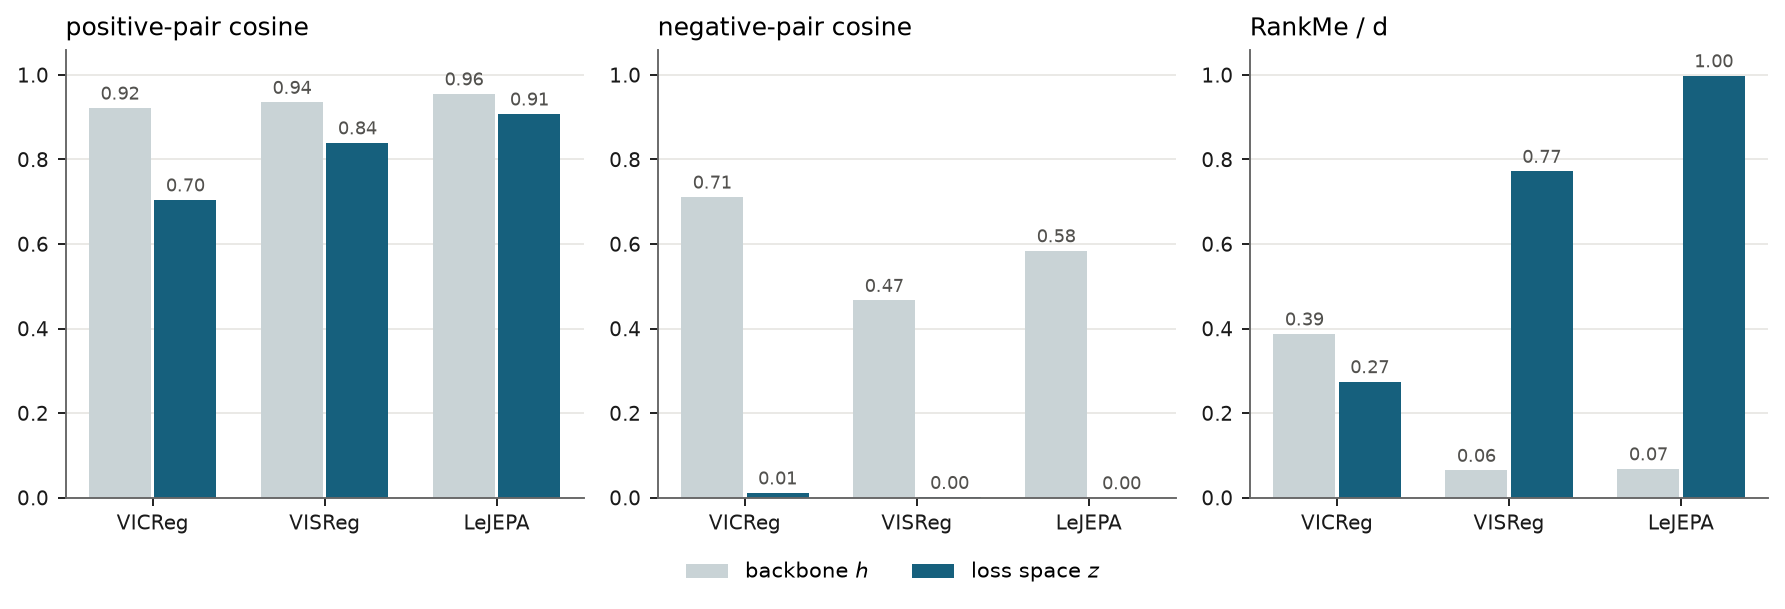
\includegraphics[width=0.8\linewidth]{figures/fig_hz_bars_no_simclr.png}
    \caption{Backbone and loss-space geometry for explicitly regularized JE-SSL methods. The projection head changes both pairwise similarities and effective rank. Specifically, the projected representation can be high-rank even when the backbone features remain low-rank.}
    \label{fig:hz_geometry}
\end{figure}


\CD{We need to cite WLD-Reg~\cite{laakom2023wld} 
DeCov~\cite{cogswell2015reducing} }


% \paragraph{Gaussian example.} Let
% \[
% Z = (Z_1,Z_2)^\top \sim \mathcal{N}(0,I_2),
% \]
% and define
% \[
% H =
% \begin{pmatrix}
% Z_1\\
% Z_2 + Z_1^2 - 1
% \end{pmatrix},
% \qquad
% p(h_1,h_2) =
% \begin{pmatrix}
% h_1\\
% h_2 - h_1^2 + 1
% \end{pmatrix}.
% \]

% Then
% \[
% p(H)=Z
% \]
% exactly. It means the projected representation is standard Gaussian. However, \(H\) is not Gaussian, since
% \[
% \mathbb{E}\!\left[(Z_2+Z_1^2-1)^3\right]=8\neq 0.
% \]
% and,
% \[
% \operatorname{Cov}(H)=\operatorname{diag}(1,3).
% \]
% Therefore, even an exact isotropic-Gaussian constraint on $Z$ does not imply
% Gaussianity or isotropy of $H$.


% \paragraph{Rank example} Let \(X\) be uniform on \(\{-1,0,1\}\), and define
% \[
% H=
% \begin{pmatrix}
% X\\
% 0
% \end{pmatrix},
% \qquad
% p(h_1,h_2)=
% \begin{pmatrix}
% h_1\\
% |h_1|
% \end{pmatrix}.
% \]

% Then
% \[
% Z=p(H)=
% \begin{pmatrix}
% X\\
% |X|
% \end{pmatrix}.
% \]
% The backbone has rank one covariance,
% \[
% \operatorname{Cov}(H)=\operatorname{diag}(2/3,0),
% \]
% while
% \[
% \operatorname{Cov}(Z)=\operatorname{diag}(2/3,2/9),
% \]
% which is full rank. Therefore, a nonlinear projector can produce a full-rank \(Z\) even though \(H\) has rank-deficient covariance. \BD{this motivates regularizing backbone directly here or after the feat learning?, im putting a note to not to forget}


\subsection{No-collapse / broad backbone representations}

In task-agnostic representation learning, different downstream tasks can benefit from different invariances, so variation discarded during pretraining may later become task-relevant~\citep{wellericsson2021, tian2020makes}. Dimensional collapse in the backbone is therefore particularly restrictive: directions suppressed there are unavailable to downstream tasks using the frozen representation. Consistent with this view, effective rank has been shown to predict downstream performance in JE-SSL~\citep{rankme2023}. Together with the mismatch in Section~\ref{sec:rel_jepa}, this motivates preventing collapse directly in the backbone representation.


\BD{paragraph about rich/lazy connection, the order could be reversed, bridge to method section is important}

\newpage

\section{Method}

Our goal is to prevent collapse in the backbone representations retained for downstream transfer. We first study a tractable two-layer linear network, where negative layer balance yields a non-collapse guarantee
and motivates an encoder-side spectral regulariser. We then extend this principle to nonlinear encoders by regularising the representation covariance directly. Finally, we apply the regulariser to joint-embedding self-supervised learning, targeting backbone representations averaged across augmented views to promote variation between images.



\subsection{Deriving a spectral anti-collapse mechanism in linear networks}




\paragraph{Linear-network setting.}
Consider a supervised dataset
$
\mathcal{D}
=
\left\{
(\mathbf{x}_n,\mathbf{y}_n)
\right\}_{n=1}^{P}
$, $
\mathbf{x}_n\in\mathbb{R}^{N_i} 
$, $
\mathbf{y}_n\in\mathbb{R}^{N_o}.
$
We model the input--output mapping using a two-layer linear network, $\widehat{\mathbf{y}}_n
=
\wb\wa\mathbf{x}_n,$
where $\wa\in\mathbb{R}^{N_h\times N_i}$ and
$\wb\in\mathbb{R}^{N_o\times N_h}$ denote the encoder and decoder weight
matrices, respectively. The network is trained on the mean-squared-error
loss
$
\mathcal{L}_{\mathrm{task}}(\wa,\wb)
=
\frac{1}{2}
\left\langle
\left\|
\wb\wa\mathbf{x}-\mathbf{y}
\right\|_2^2
\right\rangle,$
where $\langle\cdot\rangle$ denotes the empirical average over the training
set. Although the task loss depends only on the end-to-end mapping
$M=\wb\wa$, its factorisation across the two layers affects the parameter
and representation dynamics. We characterise this factorisation through
the layer-imbalance matrix
$
\Delta
=
\wb^\top\wb-\wa\wa^\top.
$
A network is said to be $\lambda$-balanced when
$
\Delta
=
\lambda\mathbf{I}_{N_h}.$
Previous work has shown that $\lambda$-balanced initialisations provide an analytically tractable framework for characterising the transition between rich and lazy learning dynamics~\citep{domine2024lazy,nam2025position}. Under unregularised gradient flow, $\Delta$ is conserved, so the layer balance remains fixed at its initial value. Prior studies have also linked these learning regimes to the rank of the learned representations \mm{not really clear here. Same prior work as above? If so, merge the two sentences, otherwise provide new references}. Motivated by this connection, we investigate whether a suitable layer balance can prevent representation collapse. We show that an appropriately chosen negative balance provides such a guarantee, and use this result to derive a regulariser that dynamically promotes the same anti-collapse property during training.

\paragraph{Balancedness anti-collapse property.}
A negative layer balance provides an explicit anti-collapse guarantee.
If $\Delta=\lambda_{\mathrm{bal}}\mathbf{I}_{N_h}$ with
$\lambda_{\mathrm{bal}}<0$, then
$
\wa\wa^\top\succeq-\lambda_{\mathrm{bal}}\mathbf{I}_{N_h},
 \text{ and }
\sigma_{\min}(\wa)\geq\sqrt{-\lambda_{\mathrm{bal}}},
$
so the encoder has full row rank. This also yields a guarantee for
the hidden representations under the assumption that, for some $\mu>0$, the input
covariance $\Sigma_x
=
\frac{1}{P}\sum_{n=1}^{P}
(\mathbf{x}_n-\bar{\mathbf{x}})
(\mathbf{x}_n-\bar{\mathbf{x}})^\top \succeq\mu\mathbf{I}_{N_i}$, with $ 
\bar{\mathbf{x}}=\frac{1}{P}\sum_{n=1}^{P}\mathbf{x}_n$.
In fact, the centered covariance of the hidden representations
$\mathbf{z}_n=\wa\mathbf{x}_n$ satisfies $\Sigma_z
=
\wa\Sigma_x\wa^\top
\succeq
-\mu\lambda_{\mathrm{bal}}\mathbf{I}_{N_h}.$
Therefore, negative layer balance prevents both complete and dimensional \mm{what do you mean by ``complete'' and ``dimensional''?} representation collapse, see Lemma~\ref{lem:balanced-non-collapse} in Appendix \ref{app:noncollapse} for a formal statement and proof.

Although a balanced initialisation prevents collapse, extending the same initialisation strategy to deep nonlinear networks is far from obvious. We therefore seek a regularised training objective that dynamically selects a negative layer balance, independently of its initial value. Motivated by this objective, we derive a regulariser that follows from a constrained optimisation problem. 

\paragraph{Selecting layer balance through regularisation.}

Among all factorisations of a fixed end-to-end mapping
$M=\wb\wa$, we look for a constrained minimiser that satisfies
$
\wb^\top\wb-\wa\wa^\top
=
-\frac{\gamma}{\lambda_{\mathrm{reg}}}
\mathbf{I}_{N_h}.$

%The regulariser therefore selects a particular $\lambda$-balanced factorisation, rather than merely penalising the magnitude of the weights.




\begin{theorem}
\label{thm:encoder-variational-balance}
Fix an end-to-end mapping $
M\in\mathbb{R}^{N_o\times N_i}$, $\gamma \geq  0$ and $\lambda_{\mathrm{reg}} \geq  0$. Let $(\wa^\star,\wb^\star)$ be a solution of \BD{i think you mean strictly greater can you check?}
\begin{equation}
\begin{aligned}
\min_{\wa,\wb}\quad&
\frac{\lambda_{\mathrm{reg}}}{2}
\left(
    \|\wa\|_F^2+\|\wb\|_F^2
\right)
-
\frac{\gamma}{2}
\log\det\left(\wa\wa^\top\right)\quad \text{subject to}\quad
\wb\wa=M,
\end{aligned}
\label{eq:encoder-constrained-problem}
\end{equation}
with
\(\wa^\star(\wa^\star)^\top\succ0\). Then,  $(\wb^\star)^\top\wb^\star
-
\wa^\star(\wa^\star)^\top
=
-\frac{\gamma}{\lambda_{\mathrm{reg}}}
\mathbf{I}_{N_h}$
\end{theorem}
The proof of Theorem~\ref{thm:encoder-variational-balance} is provided in Appendix \ref{app:opptimisation}. This motivates the following definition.
\begin{definition}[Linear SACReg]
\label{def:linear-encoder-regulariser}
Assume that $\wa\wa^\top\succ0$, $\gamma \geq  0$ and $\lambda_{\mathrm{reg}} \geq  0$. We define
\[
\mathcal{R}_{\mathrm{LSAC}}(\wa,\wb)
=
\frac{\lambda_{\mathrm{reg}}}{2}
\left(
    \|\wa\|_F^2+\|\wb\|_F^2
\right)
-
\frac{\gamma}{2}
\log\det\left(\wa\wa^\top\right),
\]
%where $\lambda_{\mathrm{reg}}$ controls the strength of the symmetric
%$L_2$ decay and $\gamma>0$ controls the log-determinant term. 
and the
corresponding training objective  $$\mathcal{L}_{\mathrm{LSAC}}(\wa,\wb)
=
\mathcal{L}_{\mathrm{task}}(\wa,\wb)
+
\mathcal{R}_{\mathrm{LSAC}}(\wa,\wb).
\label{eq:encoder-regularised-objective}$$
\end{definition}
The regulariser combines symmetric $L_2$ weight decay with a
log-determinant term acting specifically on the encoder Gram matrix. 
This placement is motivated by the non-collapse condition:
a negative layer balance bounds the encoder Gram matrix away being singular and, under the input-covariance assumption, guarantees
non-collapse of the hidden representations. The log-determinant term
penalises vanishing encoder singular values, while weight decay controls the overall weight scale.


 We next show that the balance
identified by the constrained optimisation problem also emerges
dynamically during training. For $N_h\leq N_i$ and
$\wa(0)\wa(0)^\top\succ0$, regularised gradient flow on the
mean-squared-error objective exists globally \mm{what do you mean by `exists globally'?} and preserves the
full row rank of the encoder. The task-loss terms cancel in the imbalance dynamics,
giving $\tau\dot{\Delta}
=
-2\lambda_{\mathrm{reg}}\Delta-2\gamma\mathbf{I}_{N_h}.$
Consequently,
$$\Delta(t)+\frac{\gamma}{\lambda_{\mathrm{reg}}}\mathbf{I}_{N_h}
=
e^{-2\lambda_{\mathrm{reg}}t/\tau}
\left(
\Delta(0)+\frac{\gamma}{\lambda_{\mathrm{reg}}}\mathbf{I}_{N_h}
\right).$$
Thus, independently of the dataset and initial imbalance, the network
converges exponentially with rate $2\lambda_{\mathrm{reg}}/\tau$ to \mm{a $\lambda_{\mathrm{bal}}^{\mathrm{enc}}$-balanced solution, with}
$\lambda_{\mathrm{bal}}^{\mathrm{enc}}
=-\gamma/\lambda_{\mathrm{reg}}$; see
Theorem ~\ref{thm:encoder-balance-dynamics} in Appendix \ref{app:balsel}.
For any  given balanced initialization, the network preserves it throughout training (Corollary~\ref{cor:selected-balance-persistence}). Unlike $\lambda$-balanced initialisation, which fixes the balance only
through the starting condition, the proposed objective continuously
attracts the network towards the selected balance. The ratio
$\gamma/\lambda_{\mathrm{reg}}$ determines the fixed point, while
$\lambda_{\mathrm{reg}}$ controls the rate of convergence towards it. 
% Assume $N_h\leq N_i$ and initialise the encoder with $\wa(0)\wa(0)^\top\succ0$. For the mean-squared-error objective, the regularised gradient flow exists for all $t\geq0$ and preserves encoder full row rank; see Proposition~\ref{prop:encoder-balance-dynamics}. With time scale $\tau>0$, the imbalance satisfies \[ \tau\dot{\Delta}(t) = -2\lambda_{\mathrm{reg}}\Delta(t) -2\gamma\mathbf{I}_{N_h}. \]
%The task-loss contributions cancel exactly, making the balance dynamics independent of the dataset and of the end-to-end mapping being learned.
%Solving this equation gives
%\[
%\Delta(t)
%=
%e^{-2\lambda_{\mathrm{reg}}t/\tau}\Delta(0)
%-
%%\frac{\gamma}{\lambda_{\mathrm{reg}}}
%\left(
 %   1-e^{-2\lambda_{\mathrm{reg}}t/\tau}
%\right)
%\mathbf{I}_{N_h},
%\]
%and therefore
%
%\Delta(t)
%\longrightarrow
%-\frac{\gamma}{\lambda_{\mathrm{reg}}}
%\mathbf{I}_{N_h}
%\text{as }
%t\rightarrow\infty.
%$
%Thus, the encoder-side regulariser dynamically selects the asymptotic balance $\lambda_{\mathrm{bal}}^{\mathrm{enc}}
%=
%-\frac{\gamma}{\lambda_{\mathrm{reg}}}$


%Previous work has shown that such asymmetry can substantially alter feature learning, with its effect depending on both the sign of $\lambda_{\mathrm{bal}}$ and which layer is dominant

%This construction provides a direct connection between regularisation and the rich--lazy learning regimes where balancednes ~\citep{dominé2024lazyrichexactlearning} that disucuseed in appendix \ref{app:rich_lazy}. All together, we derivation of the trace--log-determinant objective from the balance mechanism identified in the linear analysis. The resulting regulariser has an explicit preferred spectrum, controls the representation scale with a single parameter ratio and indicates where to put the regulariser, and extends the linear anti-collapse mechanism to nonlinear encoders. 

This construction connects regularisation to the layer-balance
mechanism studied in rich and lazy learning
dynamics~\citep{dominé2024lazyrichexactlearning}; see
Appendix~\ref{app:rich_lazy}.
The ratio $\gamma/\lambda_{\mathrm{reg}}$ determines the selected
balance and the corresponding lower bound on the encoder spectrum and yields a non-collapse guarantee.
For centred, whitened linear inputs, the representation covariance
equals $\wa\wa^\top$, so the encoder portion of the regulariser
is exactly a trace--log-determinant penalty on that covariance.
This equivalence motivates applying the penalty directly to the
representation covariance in nonlinear encoders, as developed next. \mm{this paragraph is a little redundant and could be incorporated in the previous one just by adding a couple of lines. I think we need to make this part more compact.}






 %In particular, \citet{kunin_2024_get} show that both upstream and downstream initializations can induce rich dynamics when the overall initialization scale is small. Although balancedness is not conserved in nonlinear networks, the initial balance between layers still helps determine the learning regime. 
 %In the following section, we inpired by the linear setting we 
 %construct a practical regulariser for nonlinear networks, where exact balance dynamics are no longer available but the same spectral anti-collapse principle, the placement of the regulariser, and the learning regime ideas can be applied.







\subsection{Spectral regularisation of nonlinear representations}
\label{sec:logdet-covariance-regulariser}
Although layer imbalance is not conserved in nonlinear networks, prior work has shown that it influences their learning dynamics~\citep{kunin_2024_get,anguita2026theory,jarvis2025theory}.
Motivated by this connection and our linear analysis, we apply
the spectral anti-collapse principle directly to the encoder's
representation covariance, preserving the encoder-side placement
without relying on exact balance dynamics. Let $z=f_\theta(x)\in\mathbb{R}^{k}$ \BD{H here too?}denote the representation
produced by a differentiable encoder $f_\theta$.
For a minibatch of size $B$, collect the representations row-wise
in $Z\in\mathbb{R}^{B\times k}$ and define $\mu=\frac{1}{B}Z^\top\mathbf{1}_B,
$\text{ }$
P_B=\mathbf{I}_B-\frac{1}{B}\mathbf{1}_B\mathbf{1}_B^\top,
$\text{ }$
\widetilde Z=P_BZ,
$\text{ }$
C_z=\frac{1}{B}\widetilde Z^\top\widetilde Z.$
Here, $\mu$ and $C_z$ are the empirical representation mean
and centred covariance, respectively.

\begin{definition}[Nonlinear SACReg]
\label{def:nonlinear-encoder-regulariser}
Let $\lambda_{\mathrm{mean}}>0$,
$\lambda_{\mathrm{cov}}>0$, $\gamma>0$, and $\varepsilon\geq0$.
Assume that $C_z+\varepsilon\mathbf{I}_k\succ0$.
We define \BD{in case your theory do not repeat calling z as features, i would call it h to be consistent with the other parts, then SACReg becomes a function of H only as you already defined empirical mean and cov above?} \mm{we have too much notation, so I am all up for reducing it following Berker's comment}
\begin{equation}
\mathcal{R}_{\mathrm{SAC}}(\mu,C_z)
=
\frac{\lambda_{\mathrm{mean}}}{2}\|\mu\|_2^2
+
\frac{\lambda_{\mathrm{cov}}}{2}\operatorname{tr}(C_z)
-
\frac{\gamma}{2}
\log\det\left(C_z+\varepsilon\mathbf{I}_k\right).
\label{eq:nonlinear-covariance-regulariser}
\end{equation}
and the
corresponding training objective  $$\mathcal{L}_{\mathrm{SAC}}(\wa,\wb)
=
\mathcal{L}_{\mathrm{task}}(\wa,\wb)
+
\mathcal{R}_{\mathrm{SAC}}(\wa,\wb).$$
\end{definition}
The covariance terms play the same roles as in the linear setting: $\lambda_{\mathrm{cov}}$ controls the total representation variance, while $\gamma$ controls the strength of the log-determinant penalty on small covariance eigenvalues. The parameter $\varepsilon$ provides numerical stabilisation. The nonlinear regulariser also includes a mean penalty, weighted by $\lambda_{\mathrm{mean}}$, which pulls the representation mean towards the origin. For a bias-free linear encoder, centred inputs produce centred representations, so no separate mean penalty is needed. Instead, a nonlinearity or a bias can produce a nonzero representation mean even when the inputs are centred. Because the trace and log-determinant terms depend only on centred covariance, they are unaffected by shifts in the representation mean. The additional $\|\mu\|_2^2$ term thus controls this otherwise unconstrained shift.
The regulariser constrains only the representation mean and
covariance; it does not directly constrain higher-order moments
or enforce Gaussianity. For a linear encoder with centred, whitened inputs and $\varepsilon=0$, the covariance penalty reduces exactly to the encoder portion of the linear regulariser, with $\lambda_{\mathrm{cov}}=\lambda_{\mathrm{reg}}$. This connection is derived in Appendix~\ref{sec:nonlinear-covariance-regularisation}.





We next characterise the regulariser's inductive bias and anti-collapse properties. The mean and trace penalties control representation location and scale, while the negative log-determinant penalises small covariance eigenvalues.


%The trace and log-determinant terms play complementary roles. The trace penalty prevents unbounded growth of the representation variance, whereas
%the negative log-determinant penalises covariance spectra containing smalleigenvalues. Indeed, if
%$\lambda_1(C_z),\ldots,\lambda_k(C_z)$ are the eigenvalues of $C_z$, then$\mathcal{R}_{\mathrm{SAC}}(\mu,C_z)
%=
%\frac{\lambda_{\mathrm{mean}}}{2}\|\mu\|^2
%+
%\frac{1}{2}
%\sum_{i=1}^{k}
%\left[
%    \lambda_{\mathrm{cov}}\lambda_i(C_z)
%    -
  %  \gamma\log\left(\lambda_i(C_z)+\varepsilon\right)
%\right].$
%Thus, the regulariser acts directly on the representation's location and on every direction of its covariance; see
%Proposition~\ref{prop:nonlinear-covariance-spectral-form} in the Appendix.

\begin{theorem}[Optimal mean and covariance]
\label{thm:nonlinear-optimal-covariance}
The unique minimizer of \(\mathcal{R}_{\mathrm{SAC}}\) over $\mu\in\mathbb R^k,\ C_z\succeq0$ is
\begin{equation}
\boxed{
\mu^\star=0,
\qquad
C_z^\star
=
\left(
    \frac{\gamma}{\lambda_{\mathrm{cov}}}
    -
    \varepsilon
\right)_{+}I_k
}\qquad  \text{ where } (a)_{+}=\max\{a,0\}. 
\label{eq:nonlinear-optimal-covariance}
\end{equation}

\end{theorem}

 Thus, the regulariser favours zero-mean representations with isotropic covariance, which is full rank when $\gamma>\lambda_{\mathrm{cov}}\varepsilon$. For $\varepsilon=0$, the preferred variance is $\gamma/\lambda_{\mathrm{cov}}$. These are the preferred moments of the regulariser alone; the task loss, network parameterisation, and minibatch rank constraints may prevent their attainment. 


\paragraph{Anti-collapse property.}
When $\varepsilon=0$, the negative log-determinant is a strict barrier against covariance collapse: $\lambda_{\min}(C_z)\rightarrow0$ implies $\mathcal{R}_{\mathrm{SAC}}(\mu,C_z)\rightarrow+\infty.$
At the other extreme, the trace term prevents unbounded growth: $\lambda_{\max}(C_z)\rightarrow+\infty$ implies $\mathcal{R}_{\mathrm{SAC}}(\mu,C_z)\rightarrow+\infty.$ The mean term supplies a third, independent barrier: $\|\mu\|\rightarrow\infty$ implies $ \mathcal{R}_{\mathrm{SAC}}(\mu,C_z)\rightarrow+\infty,$ so the representation cannot escape the regulariser by drifting off in mean instead of collapsing or exploding in covariance. 
Consequently, every finite sublevel set has bounded mean and covariance eigenvalues bounded above and away from zero; see Theorem~\ref{thm:strict-covariance-non-collapse} in Appendix \ref{sec:logdet-covariance-regulariser}. We evaluate this property experimentally in nonlinear ReLU networks, following the setup of \cite{kunin_2024_get}. Consistent with our predictions, the regularizer increases representation rank across a range of initialisation scales. \mm{this needs a reference to proper figures}



%\paragraph{Preferred mean and covariance spectrum.}
%To isolate the inductive bias of the regulariser, we first minimise
%$\mathcal{R}_{\mathrm{SAC}}$ over $\mu\in\mathbb{R}^k$ and positive-semidefinite covariance
%matrices $C_z$, independently of the task loss. Since v$\mathcal{R}_{\mathrm{SAC}}$ separates
%additively into a term depending only on $\mu$ and a term depending only on $C_z$, the two may be
%minimised independently. The resulting preferred mean and %covariance are
%\begin{equation}
%\boxed{
%\mu^\star=0,
%\qquad
%C_z^\star
%=
%\left(
%    \frac{\gamma}{\lambda_{\mathrm{cov}}}
%    -
%    \varepsilon
%\right)_{+}
%\mathbf{I}_k
%},
%\label{eq:main-preferred-covariance}
%\end{equation}
%where $(a)_{+}=\max\{a,0\}$. The preferred covariance is therefore
%full rank precisely when $\gamma>\lambda_{\mathrm{cov}}\varepsilon$, independently of $\mu^\star$.
%A complete derivation is given in
%Theorem~\ref{thm:nonlinear-optimal-covariance} in the %Appendix.


%}






% {\color{blue} \textbf{Discussion on the mean}  he linear theory (Section 5.1) never needs a mean term because its model structurally cannot produce a nonzero representation mean at all (bias-free, linear, centered input $\Rightarrow$ $\mathbb{E}[z]\equiv0$). Once you either (a) add a bias, or (b) — our case — add a nonlinearity, that guarantee breaks and $\mu$ becomes a real, independently-moving quantity that $\operatorname{tr}(C_z)/\log\det(C_z)$ still can't see. The $|\mu|^2$ term is what covers that gap in either case.}
%Next we evaluate wheather this properties empirically in the following section.
%Following the setup of \citet{kunin_2024_get}, we introduce a regularizer into a two-layer network and vary the initialization scale to investigate whether regularization produces qualitatively similar learning dynamics to those induced by initialization imbalance and the properties of this regulariser. We make three observations from our results \ref{app:resultsRelu}.
%\textbf{The regulariser's rank-raising effect depends on the learning regime.}
\paragraph{Feature learning.} Using the two-layer ReLU network setup of \cite{kunin_2021_neural}, we investigate whether regularization yields qualitatively similar learning dynamics and examine its effect on the learning regime. We find that regularization promotes feature learning across a range of initialization scales, with stronger regularization associated with more pronounced feature learning (see Figure \ref{fig:rich-Relu} in Appendix \ref{app:Two-layer}). A similar trend emerges in the self-supervised setting, where measurements of the NTK and the extent of feature learning indicate rich learning dynamics (Figure \ref{fig:rich-learning}). The Appendix provides a further discussion of how initial imbalance and regularization jointly influence the learning regime \mm{too vague, can be scratched}.


Altogether, these results suggest that SACReg promotes higher-rank representations in nonlinear networks, supporting its role as an effective anti-collapse regulariser while also preserving feature learning. 
\BD{encouraging here is too strong?} \CD{Changed to preserving}


%The nonlinear covariance regulariser preserves the spectral mechanism identified by the linear analysis,  the negative log-determinant opposes contraction of low-variance representation directions, while the trace term controls the overall scale. %These experiments therefore provide qualitative support rather than establish a formal extension of the theory. 
% {\color{red}Things we should really check here did we apply the right regular + maybe I should add the VAE results + more chats about kunin }




\subsection{Spectral anti-collapse for JE-SSL}
\label{sec:ssl}

We now apply the covariance regularizer of Section~\ref{sec:logdet-covariance-regulariser}\BD{here referring to appendix is not that good. i would write sth like: We now apply the covariance regularization principle of Section~\ref{sec:logdet-covariance-regulariser} to joint-embedding self-supervised learning.} to joint-embedding self-supervised learning. 
Given image $i$ and view $j\in\{1,\ldots,V\}$, let
\[
h_i^{(j)} = f_\theta(v_i^{(j)}),
\qquad
z_i^{(j)} = p_\phi(h_i^{(j)})
\]
denote the backbone and projected representations.
Standard JE-SSL objectives enforce invariance and prevent collapse in the projected space $z$, while downstream evaluation typically uses the backbone representation $h$. 
Motivated by the mismatch identified in Section~\ref{sec:related_work}, we regularize the spectrum of the representation that is retained for transfer.

\paragraph{Regularizing view centers.}
For each image, we first average its representations across $V$ augmented views, $\bar h_i=\frac{1}{V}\sum_{j=1}^{V} h_i^{(j)},
\qquad
\bar z_i=\frac{1}{V}\sum_{j=1}^{V} z_i^{(j)}. $
For a set of view centers
$X=\{\bar x_i\}_{i=1}^{N}\subset\mathbb{R}^d$, define
$\mu_X=\frac{1}{N}\sum_{i=1}^{N}\bar x_i,
\qquad
\Sigma_X=\frac{1}{N}\sum_{i=1}^{N}
(\bar x_i-\mu_X)(\bar x_i-\mu_X)^\top . $
We regularize view centers rather than all augmented views individually: the SSL objective is already responsible for reducing within-image variation, whereas applying the covariance regularizer directly across individual views would also reward such variation and can therefore compete with the invariance objective.

\BD{here in case we have space we can add sth like There is an additional benefit to regularizing view centers. Writing the covariance of a single-view representation as \(C=B+A\), where \(B\) is between-image covariance and \(A\) is expected within-image augmentation covariance, the covariance of an average over \(V\) views is \(B+A/V\). Thus, variance caused purely by augmentations contributes less to the anti-collapse constraint as \(V\) increases. Regularizing view centers therefore preferentially encourages non-collapse of the between-image representation, rather than allowing within-image augmentation variation to satisfy the spectral constraint.}

We call the resulting regularizer \emph{SACReg}. Our standalone SSL method,
\mbox{$\lambda$-JEPA}, applies SACReg to both the backbone and projected
representations:
\begin{tcolorbox}[
    colback=gray!14,
    colframe=black,
    boxrule=0.8pt,
    arc=2mm,
    left=3mm,
    right=3mm,
    top=1.5mm,
    bottom=1.5mm
]
\begin{equation}
\label{eq:lambda-jepa}
\begin{aligned}
\operatorname{SACReg}(X)
&=
\frac{1}{2}
\left[
\|\mu_X\|_2^2
+\operatorname{tr}(\Sigma_X)
-\log\det(\Sigma_X+\varepsilon I)
-d
\right], \\[2mm]
\mathcal L_{\lambda\text{-JEPA}}
&=
\mathcal L_{\mathrm{SSL}}(Z)
+\beta_h\,\operatorname{SACReg}(\bar H)
+\beta_z\,\operatorname{SACReg}(\bar Z).
\end{aligned}
\end{equation}
\end{tcolorbox}
The mean term centers the representation, the trace controls its overall scale, and the negative log-determinant penalizes vanishing covariance directions. 
The projected-space term provides anti-collapse where the SSL objective is optimized, while the backbone term directly protects the representation retained for downstream transfer.

When applying our regularizer to an existing SSL method that already contains its own projected-space anti-collapse mechanism, we leave its original objective unchanged and add only the backbone term,
$\beta_h\operatorname{SACReg}(\bar H)$.
In practice, when the feature dimension exceeds the number of image centers in a minibatch, we evaluate the regularizer over orthogonal lower-dimensional slices of the representation; details are given in Appendix~\ref{app:slicing}.



%Another possible choice is the log-determinant regularizer, whose
%Bregmann divergence is so called the LogDet divergence. There are many ap-
%plications of the LogDet divergence such as metric learning and Gaussian
%graphical models . However, the log-determinant regularizer is less popular in online prediction and it is unclear how to derive general and non-trivial regretbounds when using the FTRL with the log-determinant regularizer, as posedas an open problem in \cite{}. 

% \end{remark}

\section{Experiments}

\subsection{Setup}
\label{sec:exp-setup}
We use ImageNet-1k (CITE) for large-scale image SSL, ImageNet-100 for controlled experiments, and Kinetics-710 (CITE) for video, where we follow LeVJEPA and train on a class-balanced 20\% subset. The controlled experiments use ViT-S. The large-scale runs use ViT-S and ViT-B for 100 and 400 epochs on images, and up to 1{,}085 epochs on video. Due to compute limitations, we do not retune hyperparameters for the 400-epoch ImageNet-1k or 1{,}085-epoch video runs, which we use primarily to assess how the method scales with extended training rather than as tuned benchmark results. For evaluation we follow the standard frozen-feature protocols: the linear-probe and kNN protocol of the Lightly benchmark on ImageNet-1k, the VISReg protocol for transfer, and the LeVJEPA protocol for video; details are given in Appendix~\ref{app:exp-details}. Whenever public checkpoints trained under one codebase are available (OK-AI CITATION), we evaluate them under the same protocol; otherwise we report the published numbers. We set the loss weights using the gradient-based calibration procedure described in Appendix~\ref{app:loss-weights}.

\subsection{Performance at scale}
Table~\ref{tab:in1k-main} reports linear-probe and kNN accuracy on ImageNet-1k, and Table~\ref{tab:transfer-main} the average transfer accuracy over eight classification datasets. We compare most directly with LeJEPA and VISReg, the related explicitly regularized JE-SSL methods. We additionally include DINO and iBOT as established SSL methods to contextualize the quality of the learned representations, rather than as direct competitors.

At 100 epochs, where training length is matched, our standalone objective substantially outperforms the directly related explicitly regularized methods. On ImageNet-1k linear probing, our ViT-S improves over LeJEPA by 7.2 points, while our ViT-B improves over LeJEPA and VISReg by 4.5 and 3.9 points, respectively. The gains are larger on transfer: +8.9 points over LeJEPA for ViT-S, and +6.7 and +4.5 points over LeJEPA and VISReg for ViT-B. At the same time, performance remains comparable to DINO and iBOT: ViT-S is within 0.3 points of DINO on linear probing, ViT-B slightly exceeds DINO, and our models match or exceed all reported 100-epoch reference points on the transfer benchmark. At longer training, available checkpoints in the literature use different training lengths, so we report our 400 epoch results as context rather than as strictly epoch matched comparisons. Our 400-epoch models continue to improve significantly in both linear probing and transfer; notably, ViT-B remains ahead of the 400-epoch VISReg checkpoint while coming within roughly one point of the published DINO and iBOT transfer results, and ViT-S reaches within 0.2 points of their 300-epoch transfer checkpoints.

\BD{talk about knn or remove?}
kNN accuracy is the main exception: our models remain 5--9 points below DINO and iBOT despite substantially stronger linear-probe and transfer performance\BD{will investigate/discuss}. Overall, extending training from 100 to 400 epochs consistently improves linear and transfer accuracy at both model sizes, indicating that the objective continues to benefit from longer pretraining.

\subsection{Beyond image SSL: the recipe on video}
\label{sec:exp-video}
We apply the same objective to video by replacing the loss inside the LeVJEPA training pipeline and keeping their model, optimizer and data pipeline. Frozen encoders are evaluated on three benchmarks that test different content: ImageNet-1k (a single image; appearance), Something-Something-v2 (CITE) (short clips of human--object interactions such as \emph{putting something into something}, where the label is the temporal relation), and Kinetics-400 (CITE) (short real-world clips such as \emph{playing guitar}; appearance and context). Table~\ref{tab:video-main} compares our ViT-S at 240 epochs and ViT-B at 240 and 1{,}085 epochs with LeVJEPA, V-JEPA~2 (CITE) and VideoMAEv2 (CITE) at matched epochs. On ImageNet-1k our encoders are ahead of LeVJEPA and V-JEPA~2 at 240 epochs for both sizes; at 1{,}085 epochs we stay below LeVJEPA and above the other two. The largest effect is on the temporal benchmark: on SSv2 our ViT-B is 13.5 points above LeVJEPA at 240 epochs and 7.9 points above its 1{,}085-epoch model, and ahead of V-JEPA~2 and VideoMAEv2 as well. On Kinetics-400 we are within 1.2 points of LeVJEPA with the same mean-pooled linear probe; since LeVJEPA does not release its probe settings, we also report the linear probe on the CLS token and the attentive probe.
% TODO cite: LeVJEPA, V-JEPA 2, VideoMAEv2, SSv2, Kinetics.


\subsection{Controlled experiments on ImageNet-100: the regularizer on other methods}
\label{sec:exp-in100}
The large-scale runs use the regularizer in both spaces. To isolate its effect at the backbone, we train six augmentation-based methods on ImageNet-100 (LeJEPA, VICReg, SimCLR, DINO, BYOL, VISReg) with their own objectives, and once more with $\beta_{\mathrm{h}}\mathcal{R}_{\mathrm{ctr}}$ added at the backbone and everything else unchanged. The weight is not tuned per method: it is set so that the added term contributes a fixed small fraction of the gradient on the backbone (See Appendix~\ref{app:loss-weights}). Our own objective is included with and without the backbone term.

Figure~\ref{fig:constraint-mismatch} confirms on these models what Section~\ref{sec:related_work} argued: each method's own constraint holds after the projector and not at the backbone (LeJEPA's Gaussianity, VICReg's variance criterion, SimCLR's alignment). Figure~\ref{fig:two-space-audit} shows what the backbone regularizer changes. At the backbone, the effective rank rises from 6--24\% of the feature dimension to 51--86\%, and the rank of the between-image covariance rises with it; after the projector the same statistics barely move. Downstream performance follows the backbone, not the loss space: kNN accuracy improves for every method, by 3 to 13 points, and linear-probe accuracy improves for all but VICReg, where it is unchanged. Figure~\ref{fig:rich-learning} shows that this capacity is not obtained by freezing feature learning: the backbone features move far from their initialization and the tangent kernel keeps changing during training, as for the unregularized model. As a complementary control, Appendix~\ref{app:lejepa} shows whether simply adding LeJEPA's own anti-collapse regularizer to the backbone is sufficient. We find that despite improving its Gaussianity diagnostics, it does not improve downstream performance.


\subsection{Augmentation thickness}

\label{sec:exp-thickness}
Let $Q$ denote the source image and let $H$ vary over augmented views of $Q$. We decompose its covariance into

\begin{equation}
    C_h = B_h + A_h,
    \qquad
    B_h = \operatorname{Cov}\!\left(\mathbb{E}[H \mid Q]\right),
    \qquad
    A_h = \mathbb{E}\!\left[\operatorname{Cov}(H \mid Q)\right].
\end{equation}
Here, $B_h$ measures variation between images, while $A_h$ measures variation across views of the same image. $A_h$ alone is difficult to interpret: the same amount of view variation matters differently when image centers are well separated or concentrated. We therefore measure augmentation variation relative to between-image variation and define

\begin{equation}
    \Theta_h
    =
    B_h^{\dagger/2} A_h B_h^{\dagger/2}.
    \label{eq:thickness}
\end{equation}
Along any direction $a$ with nonzero between-image variance,

\begin{equation}
    \theta_h(a)
    =
    \frac{a^\top A_h a}{a^\top B_h a}.
\end{equation}
We call $\Theta_h$ the \emph{augmentation thickness} of the retained representation.

Thickness is not a quantity that should simply be minimized. Consider a centered image-level target $y$ with $\|y\|_{L_2}\leq1$. Let
\begin{equation}
    E_{\mathcal A}(y)
    =
    \min_f
    \mathbb{E}\!\left[(y(Q)-f(V))^2\right]
\end{equation}

be the irreducible error of predicting $y$ from a single augmented view, and let $d_h(y)$ be the error of the best linear prediction from the backbone image centers.

\begin{theorem}[Two sides of augmentation thickness]
\label{thm:thickness}
Assume the image-center covariance is whitened. Then,
\begin{equation}
    d_h(y)
    \geq
    \left(
        \sqrt{E_{\mathcal A}(y)}
        -
        \sqrt{\|\Theta_h\|_{\mathrm{op}}}
    \right)_+ .
    \label{eq:too-thin}
\end{equation}
% Moreover, let $a^\top m_h(Q)$ be the best linear prediction of $y$ from the image centers. Then the best linear prediction error from a single view representation $H$ is
Moreover, let $a$ be the coefficient vector of the best linear prediction of $y$ from the image centers. Then the best linear prediction error from a single view representation $H$ is
\begin{equation}
    \inf_u
    \mathbb{E}\!\left[(y-u^\top H)^2\right]
    =
    d_h(y)^2
    +
    a^\top
    \Theta_h (I+\Theta_h)^{-1} a.
    \label{eq:too-thick}
\end{equation}
For fixed image-center organization and task direction, this error term increases as augmentation thickness increases.
\end{theorem}

The proof is given in Appendix~\ref{app:thickness}. The first result shows that making $H$ too invariant can remove differences between images that are affected by the augmentations. The second shows that, for the same organization across image centers, more variation across views makes prediction from a view harder. Thus, thickness captures a trade-off: we do not want to remove all augmentation variation, but we also do not want it to dominate the representation.
\paragraph{Thickness and the regularizer.}
% Sources: results/diag/e23_retro_spaces.csv (Theta_h per model); C8 (fig_org_vs_sensitivity,
% agreed 2026-08-13); E36 card (the centroid vs residual split, RAW).
We estimate $\Theta_h$ from eight augmented views per image (Appendix~\ref{app:exp-details}). Figure~\ref{fig:thickness-gain} places every ImageNet-100 model in the plane of thickness and accuracy: the backbone regularizer makes $h$ thicker for every method, and accuracy rises at the same time, so the gain is not obtained by making the retained representation more invariant. Figure~\ref{fig:organization-sensitivity} looks at the same models through Eq.~\eqref{eq:too-thick}, per class: with the regularizer, the view-sensitivity term along the class direction grows slightly while the organization of the image centers improves more, so the single-view error falls (for 96 of 100 classes in our model). The regularized backbone therefore keeps more augmentation-dependent variation along class directions, and its accuracy gain comes from better organized image centers rather than from that variation.



% Let $Q$ denote the source image and let $H$ vary over augmented views of $Q$. We decompose its covariance into

% \begin{equation}
%     C_h = B_h + A_h,
%     \qquad
%     B_h = \operatorname{Cov}\!\left(\mathbb{E}[H \mid Q]\right),
%     \qquad
%     A_h = \mathbb{E}\!\left[\operatorname{Cov}(H \mid Q)\right].
% \end{equation}
% Here, $B_h$ measures variation between images, while $A_h$ measures variation across views of the same image. $A_h$ alone is difficult to interpret: the same amount of view variation matters differently when image centers are well separated or concentrated. We therefore measure augmentation variation relative to between-image variation and define

% \begin{equation}
%     \Theta_h
%     =
%     B_h^{\dagger/2} A_h B_h^{\dagger/2}.
%     \label{eq:thickness}
% \end{equation}
% Along any direction $a$ with nonzero between-image variance,

% \begin{equation}
%     \theta_h(a)
%     =
%     \frac{a^\top A_h a}{a^\top B_h a}.
% \end{equation}
% We call $\Theta_h$ the \emph{augmentation thickness} of the retained representation.

% Thickness is not a quantity that should simply be minimized. Consider a centered image-level target $y$ with $\|y\|_{L_2}\leq1$. Let
% \begin{equation}
%     E_{\mathcal A}(y)
%     =
%     \min_f
%     \mathbb{E}\!\left[(y(Q)-f(V))^2\right]
% \end{equation}

% % be the best possible prediction error for $y$ from a single augmented view
% be the irreducible error of predicting $y$ from a single augmented view, and let $d_h(y)$ be the error of the best linear prediction from the backbone image centers.

% \begin{theorem}[Two sides of augmentation thickness]
% \label{thm:thickness}
% Assume the image-center covariance is whitened. Then,
% \begin{equation}
%     d_h(y)
%     \geq
%     \left(
%         \sqrt{E_{\mathcal A}(y)}
%         -
%         \sqrt{\|\Theta_h\|_{\mathrm{op}}}
%     \right)_+ .
%     \label{eq:too-thin}
% \end{equation}
% % Moreover, let $a^\top m_h(Q)$ be the best linear prediction of $y$ from the image centers. Then the best linear prediction error from a single view representation $H$ is
% Moreover, let $a$ be the coefficient vector of the best linear prediction of $y$ from the image centers. Then the best linear prediction error from a single view representation $H$ is
% \begin{equation}
%     \inf_u
%     \mathbb{E}\!\left[(y-u^\top H)^2\right]
%     =
%     d_h(y)^2
%     +
%     a^\top
%     \Theta_h (I+\Theta_h)^{-1} a.
%     \label{eq:too-thick}
% \end{equation}
% For fixed image-center organization and task direction, this error term increases as augmentation thickness increases.
% \end{theorem}

% The proof is given in Appendix~\ref{app:thickness}. The first result shows that making $H$ too invariant can remove differences between images that are affected by the augmentations. The second shows that, for the same organization across image centers, more variation across views makes prediction from a view harder. Thus, thickness captures a trade-off: we do not want to remove all augmentation variation, but we also do not want it to dominate the representation.


% =========================
% Main results: 100 epochs
% =========================
\begin{table}[t]
\centering
\small
\begin{tabular}{llrr}
\toprule
Method & Backbone & Linear & Transfer Avg. \\
\midrule
LeJEPA & ViT-S/16 & 62.5 & 68.7 \\
DINO   & ViT-S/16 & 70.0 & 75.7 \\
iBOT   & ViT-S/16 & 70.9 & 75.9 \\
\textbf{$\bm{\lambda}$-JEPA} & \textbf{ViT-S/16}
& \textbf{69.7} & \textbf{77.6} \\
\midrule
LeJEPA & ViT-B/16 & 69.7 & 74.2 \\
DINO   & ViT-B/16 & 73.9 & 78.3 \\
iBOT   & ViT-B/16 & 77.0 & 80.7 \\
VISReg & ViT-B/16 & 70.3 & 76.4 \\
\textbf{$\bm{\lambda}$-JEPA} & \textbf{ViT-B/16}
& \textbf{74.2} & \textbf{80.9} \\
\bottomrule
\end{tabular}
\caption{
ImageNet-1k 100-epoch results. ImageNet-1k linear probing accuracy,
together with average linear-probe transfer accuracy over DTD, Aircraft,
Cars, CIFAR10, CIFAR100, Flowers, Food and Pets. ImageNet-1k results are
evaluated under our common protocol; transfer results are evaluated under
the matched VISReg protocol. See Appendix~\ref{app:detailed-results} for
detailed transfer results.
}
\label{tab:main-results}
\end{table}


% =========================
% Longer training
% =========================
\begin{table}[t]
\centering
\small
\begin{tabular}{llrrr}
\toprule
Method & Backbone & Ep. & Linear & Transfer Avg. \\
\midrule
LeJEPA & ViT-S/16 & 300 & 66.4 & 71.9 \\
DINO   & ViT-S/16 & 300 & 73.8 & 79.4 \\
iBOT   & ViT-S/16 & 300 & 75.2 & 79.5 \\
\textbf{$\bm{\lambda}$-JEPA} & \textbf{ViT-S/16} & \textbf{400}
& \textbf{72.3} & \textbf{79.3} \\
\midrule
LeJEPA & ViT-B/16 & 300 & 72.4 & 75.2 \\
DINO   & ViT-B/16 & 300 & 75.2 & 79.3 \\
iBOT   & ViT-B/16 & 300 & 78.6 & 82.3 \\
MoCo v3$^\ddag$ & ViT-B/16 & 300 & 75.9 & 80.5 \\
DINO$^\ddag$    & ViT-B/16 & 400 & 77.2 & 83.1 \\
iBOT$^\ddag$    & ViT-B/16 & 400 & 78.5 & 83.2 \\
VISReg$^\ddag$  & ViT-B/16 & 400 & 74.6 & 79.1 \\
\textbf{$\bm{\lambda}$-JEPA} & \textbf{ViT-B/16} & \textbf{400}
& \textbf{76.0} & \textbf{82.0} \\
\bottomrule
\end{tabular}
\caption{
Longer-training results. ImageNet-1k linear probing accuracy, together
with average linear-probe transfer accuracy. Longer-training public SSL
checkpoints are included as context. $^\ddag$ Transfer numbers are
reported by VISReg; other transfer results are evaluated by us under the
matched VISReg protocol. See Appendix~\ref{app:detailed-results} for
detailed transfer results.
}
\label{tab:long-training-results}
\end{table}

% % =========================
% % ImageNet-1k: Linear + kNN
% % =========================
% % =========================
% % ImageNet-1k: Linear + kNN
% % =========================
% \begin{table}[h]
% \centering
% \small
% \begin{tabular}{llrrr}
% \toprule
% Method & Backbone & Ep. & Linear & kNN \\
% \midrule
% LeJEPA (OK-AI) & ViT-S/16 & 100 & 62.5 & 45.5 \\
% DINO (OK-AI) & ViT-S/16 & 100 & 70.0 & 64.7 \\
% iBOT (OK-AI) & ViT-S/16 & 100 & 70.9 & 65.7 \\
% \textbf{$\bm{\lambda}\text{-JEPA}$} & \textbf{ViT-S/16} & \textbf{100} & \textbf{69.7} & \textbf{59.2} \\
% \midrule
% LeJEPA (OK-AI) & ViT-S/16 & 300 & 66.4 & 51.5 \\
% DINO (OK-AI) & ViT-S/16 & 300 & 73.8 & 71.0 \\
% iBOT (OK-AI) & ViT-S/16 & 300 & 75.2 & 71.5 \\
% \textbf{$\bm{\lambda}\text{-JEPA}$} & \textbf{ViT-S/16} & \textbf{400} & \textbf{72.3} & \textbf{62.9} \\
% \midrule
% LeJEPA (OK-AI) & ViT-B/16 & 100 & 69.7 & 51.3 \\
% DINO (OK-AI) & ViT-B/16 & 100 & 73.9 & 69.4 \\
% iBOT (OK-AI) & ViT-B/16 & 100 & 77.0 & 72.9 \\
% VISReg & ViT-B/16 & 100 & 70.3 & 52.5 \\
% \textbf{$\bm{\lambda}\text{-JEPA}$} & \textbf{ViT-B/16} & \textbf{100} & \textbf{74.2} & \textbf{64.3} \\
% \midrule
% LeJEPA (OK-AI) & ViT-B/16 & 300 & 72.4 & 59.4 \\
% DINO (OK-AI) & ViT-B/16 & 300 & 75.2 & 73.5 \\
% iBOT (OK-AI) & ViT-B/16 & 300 & 78.6 & 77.0 \\
% MoCo v3 & ViT-B/16 & 300 & 75.9 & 68.2 \\
% DINO & ViT-B/16 & 400 & 77.2 & 73.3 \\
% iBOT & ViT-B/16 & 400 & 78.5 & 74.8 \\
% VISReg & ViT-B/16 & 400 & 74.6 & 60.0 \\
% \textbf{$\bm{\lambda}\text{-JEPA}$} & \textbf{ViT-B/16} & \textbf{400} & \textbf{76.0} & \textbf{68.6} \\
% \bottomrule
% \end{tabular}
% \caption{ImageNet-1k linear probing and kNN top-1 accuracy. OK-AI rows
% are evaluated under our common protocol; longer-training public SSL
% checkpoints are included as context.}
% \label{tab:in1k-main}
% \end{table}

% % =========================
% % ImageNet SSL Transfer
% % =========================
% % =========================
% % ImageNet SSL Transfer
% % =========================
% \begin{table}[t]
% \centering
% \small
% \begin{tabular}{llrr}
% \toprule
% Method & Backbone & Ep. & Transfer Avg. \\
% \midrule
% LeJEPA (OK-AI) & ViT-S/16 & 100 & 68.7 \\
% DINO (OK-AI) & ViT-S/16 & 100 & 75.7 \\
% iBOT (OK-AI) & ViT-S/16 & 100 & 75.9 \\
% \textbf{$\bm{\lambda}\text{-JEPA}$} & \textbf{ViT-S/16} & \textbf{100} & \textbf{77.6} \\
% \midrule
% LeJEPA (OK-AI) & ViT-S/16 & 300 & 71.9 \\
% DINO (OK-AI) & ViT-S/16 & 300 & 79.4 \\
% iBOT (OK-AI) & ViT-S/16 & 300 & 79.5 \\
% \textbf{$\bm{\lambda}\text{-JEPA}$} & \textbf{ViT-S/16} & \textbf{400} & \textbf{79.3} \\
% \midrule
% LeJEPA (OK-AI) & ViT-B/16 & 100 & 74.2 \\
% DINO (OK-AI) & ViT-B/16 & 100 & 78.3 \\
% iBOT (OK-AI) & ViT-B/16 & 100 & 80.7 \\
% VISReg & ViT-B/16 & 100 & 76.4 \\
% \textbf{$\bm{\lambda}\text{-JEPA}$} & \textbf{ViT-B/16} & \textbf{100} & \textbf{80.9} \\
% \midrule
% LeJEPA (OK-AI) & ViT-B/16 & 300 & 75.2 \\
% DINO (OK-AI) & ViT-B/16 & 300 & 79.3 \\
% iBOT (OK-AI) & ViT-B/16 & 300 & 82.3 \\
% MoCo v3$^\ddag$ & ViT-B/16 & 300 & 80.5 \\
% DINO$^\ddag$ & ViT-B/16 & 400 & 83.1 \\
% iBOT$^\ddag$ & ViT-B/16 & 400 & 83.2 \\
% VISReg$^\ddag$ & ViT-B/16 & 400 & 79.1 \\
% \textbf{$\bm{\lambda}\text{-JEPA}$} & \textbf{ViT-B/16} & \textbf{400} & \textbf{82.0} \\
% \bottomrule
% \end{tabular}
% \caption{Average linear-probe transfer accuracy over DTD, Aircraft,
% Cars, CIFAR10, CIFAR100, Flowers, Food and Pets. $^\ddag$Numbers reported
% by the VISReg paper; other rows are evaluated by us under the matched
% VISReg transfer protocol. For the detailed table, see Appendix~\ref{app:detailed-results}}
% \label{tab:transfer-main}
% \end{table}


% =========================
% Video SSL
% =========================
\begin{table}[h]
\centering
\small
\begin{tabular}{llrrrr}
\toprule
Method & Backbone & Ep. & IN-1k & SSv2 & K400 \\
\midrule
LeVJEPA & ViT-S/16 & 240 & 39.4 & --- & --- \\
V-JEPA 2 & ViT-S/16 & 240 & 38.7 & --- & --- \\
\textbf{$\bm{\lambda}\text{-JEPA}$} & \textbf{ViT-S/16} & \textbf{240}
& \textbf{46.8} & \textbf{37.3} & \textbf{40.0} \\
\midrule
VideoMAEv2 & ViT-B/16 & 240 & 47.1 & --- & --- \\
V-JEPA 2 & ViT-B/16 & 240 & 51.6 & --- & --- \\
LeVJEPA & ViT-B/16 & 240 & 50.7 & 30.4 & --- \\
\textbf{$\bm{\lambda}\text{-JEPA}$} & \textbf{ViT-B/16} & \textbf{240}
& \textbf{52.9} & \textbf{43.9} & \textbf{44.2} \\
\midrule
VideoMAEv2 & ViT-B/16 & --- & 53.4 & 43.6 & 37.4 \\
V-JEPA 2 & ViT-B/16 & --- & 51.6 & 42.5 & 40.7 \\
LeVJEPA & ViT-B/16 & 1085 & 61.0 & 40.4 & 44.6 \\
\textbf{$\bm{\lambda}\text{-JEPA}$} & \textbf{ViT-B/16} & \textbf{1085}
& \textbf{57.1} & \textbf{48.3} & \textbf{45.7} \\
\bottomrule
\end{tabular}
\caption{
Video SSL results on ImageNet-1k, Something-Something-v2, and Kinetics-400. $\lambda$-JEPA consistently improves video transfer performance, with strong gains on Something-Something-v2.
}
\end{table}

% % =========================
% % Video SSL
% % =========================
% \begin{table}[h]
% \centering
% \small
% \begin{tabular}{llrrrr}
% \toprule
% Method & Backbone & Ep. & IN-1k & SSv2 & K400 \\
% \midrule
% LeVJEPA & ViT-S/16 & 240 & 39.4 & --- & --- \\
% V-JEPA 2 & ViT-S/16 & 240 & 38.7 & --- & --- \\
% \textbf{$\bm{\lambda}\text{-JEPA}$} & \textbf{ViT-S/16} & \textbf{240}
% & \textbf{46.8} & \textbf{37.3} & \textbf{38.3 mean pool} \textbf{40.0 cls}  \\
% \midrule
% VideoMAEv2 & ViT-B/16 & 240 & 47.1 & --- & --- \\
% V-JEPA 2 & ViT-B/16 & 240 & 51.6 & --- & --- \\
% LeVJEPA & ViT-B/16 & 240 & 50.7 & 30.4 & --- \\
% \textbf{$\bm{\lambda}\text{-JEPA}$} & \textbf{ViT-B/16} & \textbf{240} & \textbf{52.9} & \textbf{43.9} & \textbf{41.8 (mean pool)} \textbf{44.2 cls} \\
% \midrule
% VideoMAEv2 & ViT-B/16 & --- & 53.4 & 43.6 & 37.4 \\
% V-JEPA 2 & ViT-B/16 & --- & 51.6 & 42.5 & 40.7 \\
% LeVJEPA & ViT-B/16 & 1085 & 61.0 & 40.4 & 44.6 \\
% \midrule
% \textbf{$\bm{\lambda}\text{-JEPA}$} & \textbf{ViT-B/16} & \textbf{1085} & \textbf{57.1} &
% \textbf{48.3} &
% \makecell[l]{\textbf{43.4} (mean pooling + linear)\\
%              \textbf{62.0} (attention + linear)\\
%              \textbf{45.7} (cls + linear )}
% \\
% \bottomrule
% \end{tabular}

% \caption{
% caption}
% \label{tab:video-main}
% \end{table}


% =========================
% Fig. 1: Z/H constraint mismatch
% =========================
\begin{figure}[h]
    \centering
    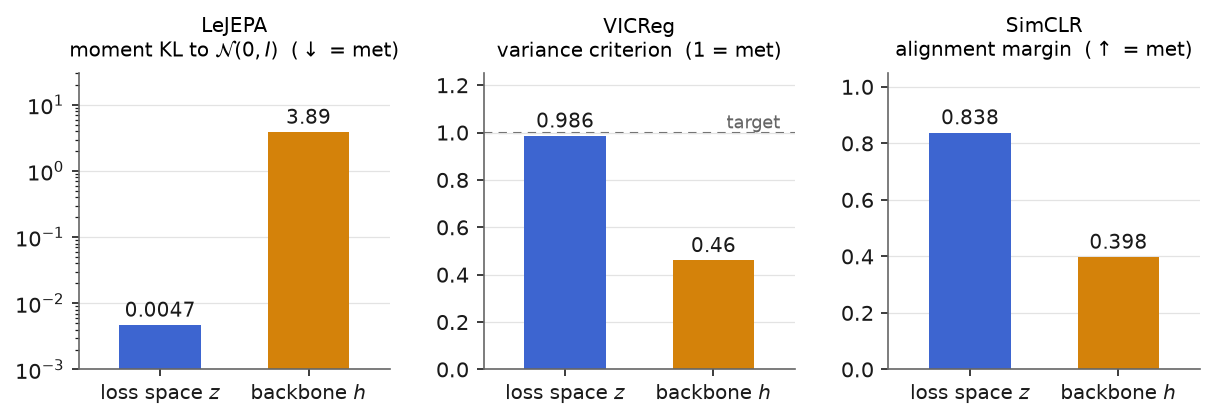
\includegraphics[width=\linewidth]{figures/fig_discrepancy.png}
    \caption{
    Constraints imposed in the projected space $Z$ do not hold in the same way at the retained backbone representation $H$. We measure each method's own training constraint for LeJEPA, VICReg, and SimCLR (THIS GOES TO FIG1 AROUND INTRO?).
    }
    \label{fig:constraint-mismatch}
\end{figure}



% =========================
% Two-space capacity audit
% =========================
\begin{figure*}[h]
    \centering
    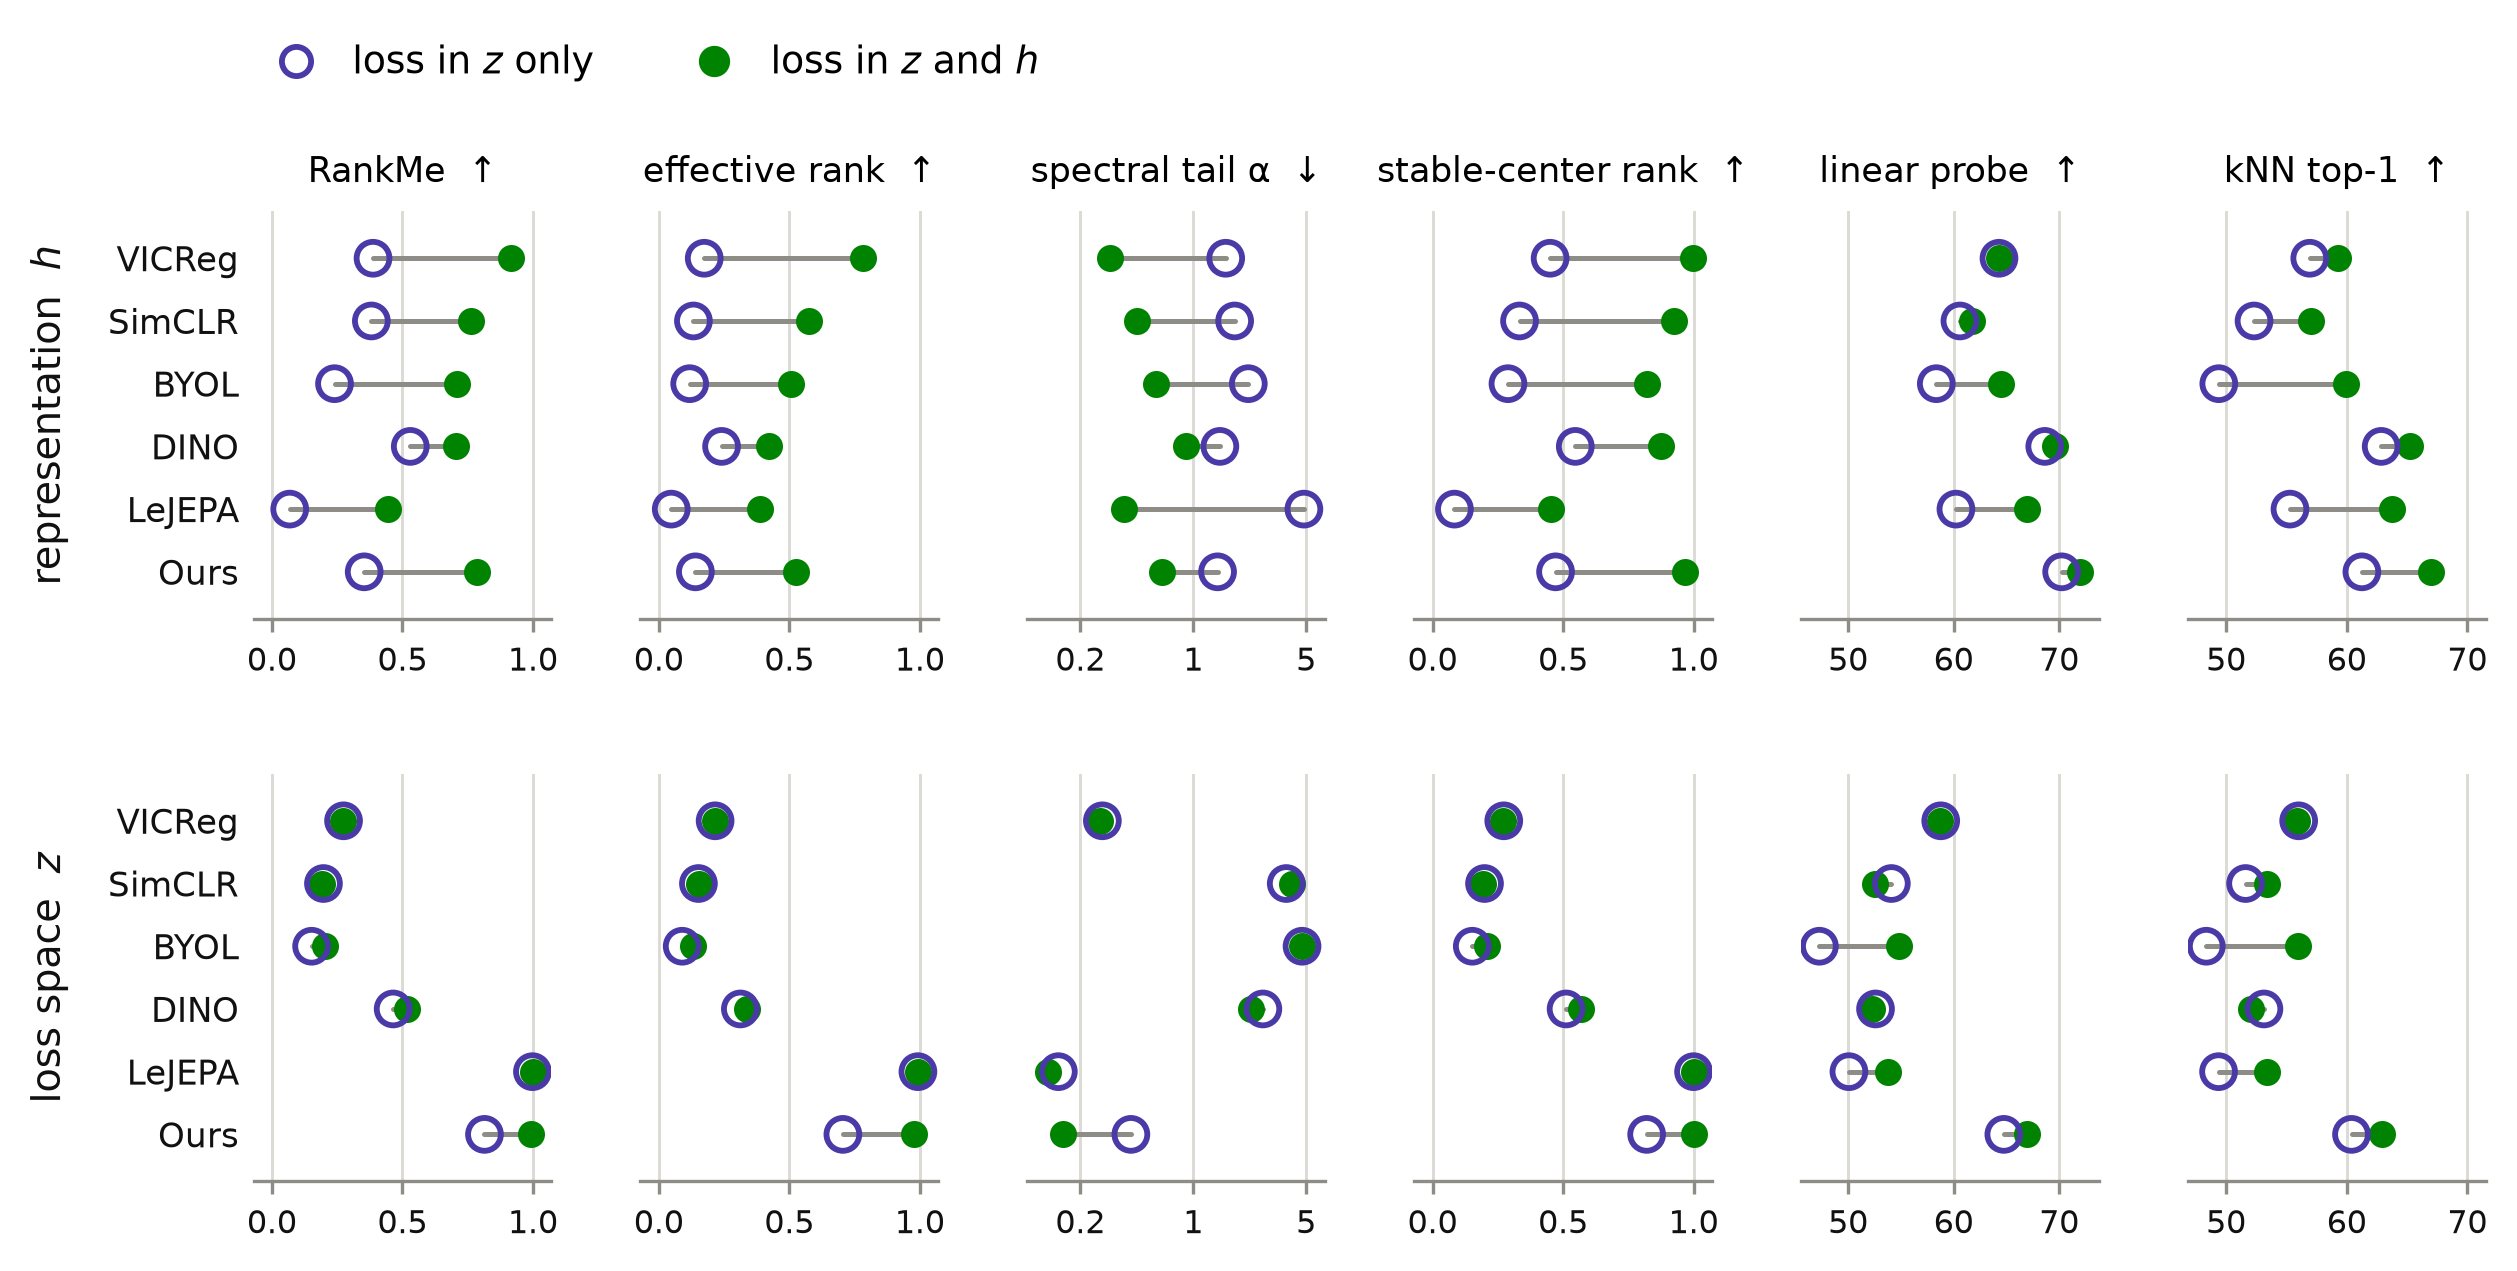
\includegraphics[width=\textwidth]{figures/in100_two_space_audit.png}
    \caption{
    Effect of backbone spectral regularization across SSL methods.
    The intervention substantially increases backbone capacity and improves downstream probes, while the projected representation $Z$ changes much less.
    }
    \label{fig:two-space-audit}
\end{figure*}

% % =========================
% % Layerwise treatment analysis
% % =========================
% \begin{figure*}[h]
%     \centering
%     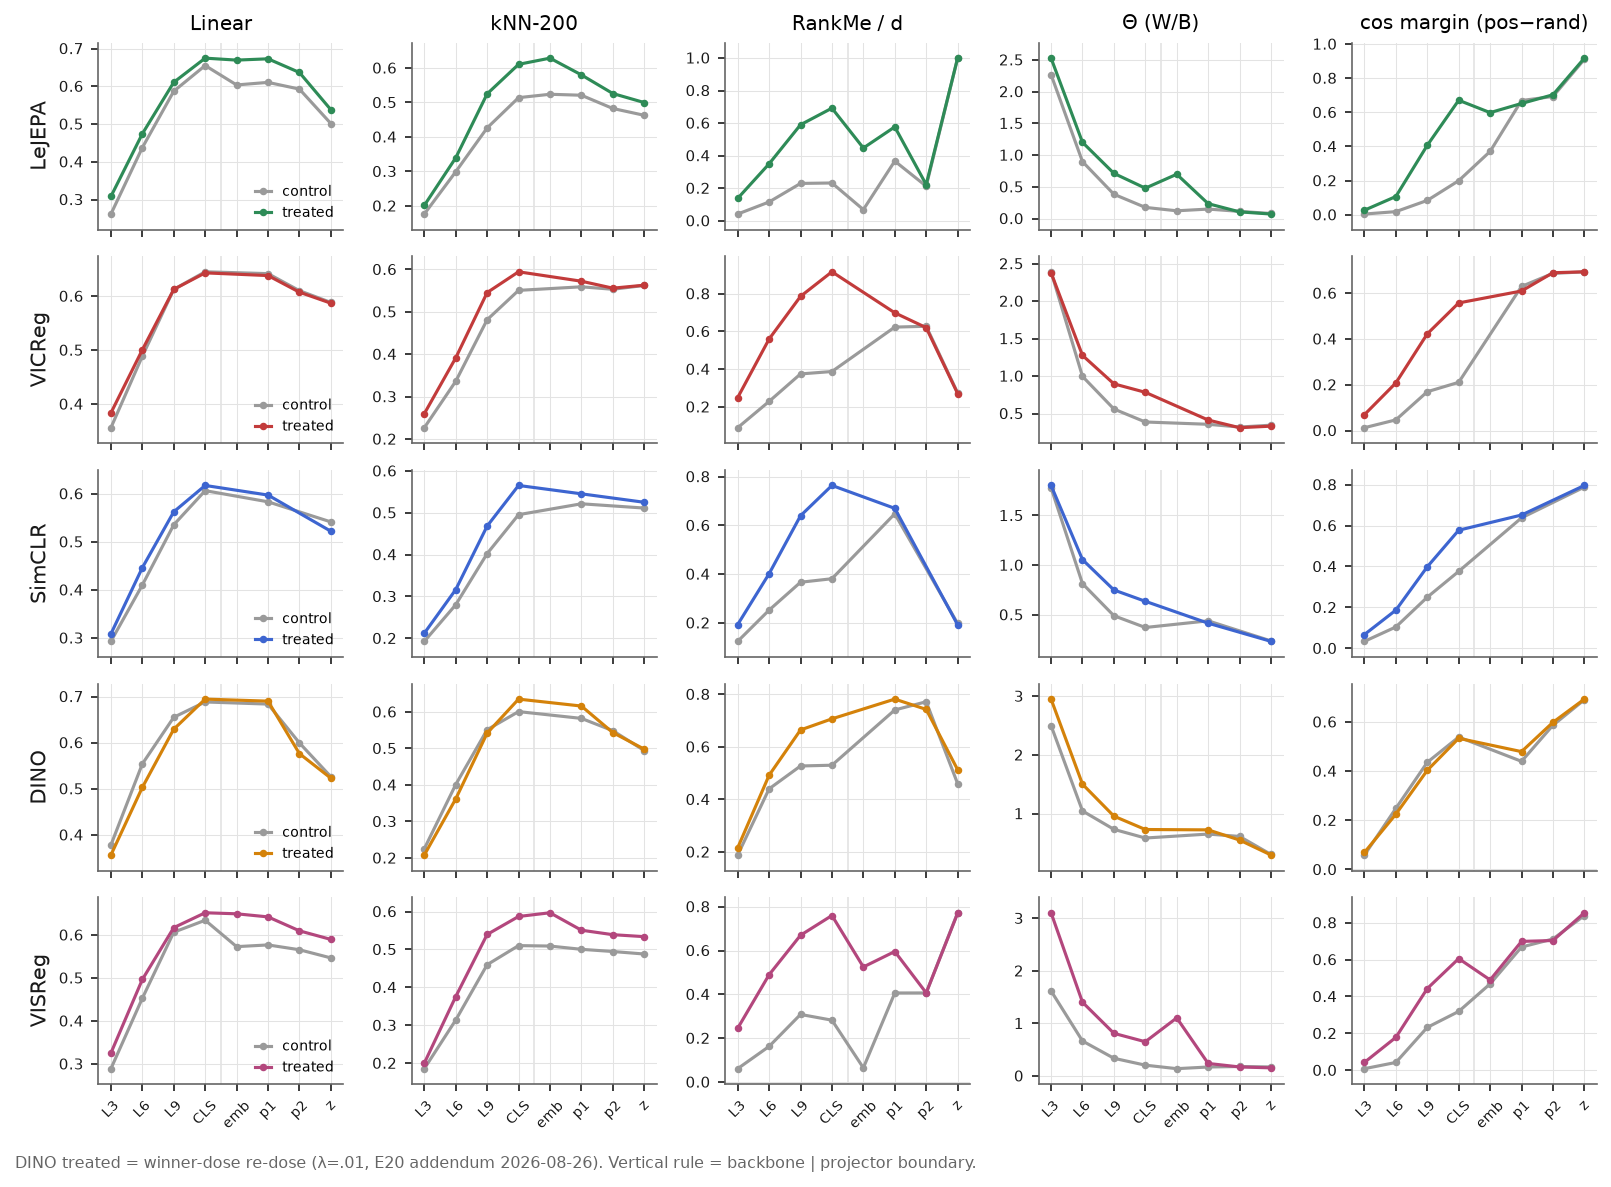
\includegraphics[width=\textwidth]{figures/fig_treatment_main.png}
%     \caption{
%     Layerwise effect of backbone spectral regularization across SSL methods. We report downstream performance, usable rank, augmentation thickness, and view-agreement statistics from intermediate backbone layers through the projector.
%     }
%     \label{fig:layerwise-treatment}
% \end{figure*}


% =========================
% Accuracy vs augmentation thickness
% =========================
\begin{figure*}[h]
    \centering
    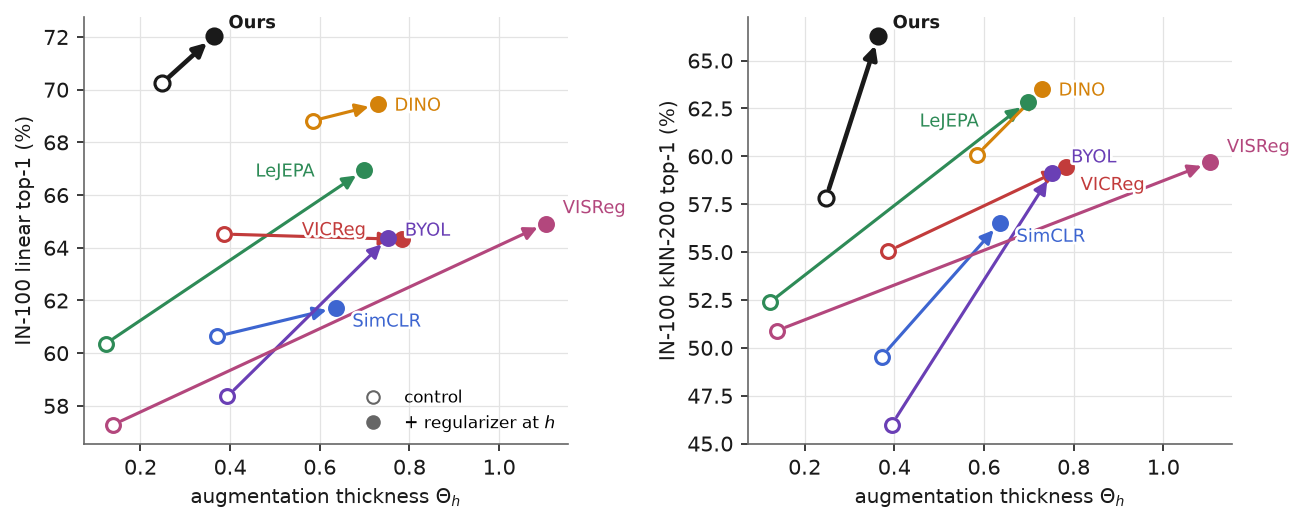
\includegraphics[width=0.82\textwidth]{figures/fig_treatment_arrows.png}
    \caption{
    Adding the backbone spectral regularizer improves linear and kNN
    accuracy while augmentation thickness in $H$ increases. The gain is therefore not obtained by making the retained representation more invariant.
    }
    \label{fig:thickness-gain}
\end{figure*}


% =========================
% Organization vs sensitivity
% =========================
\begin{figure*}[h]
    \centering
    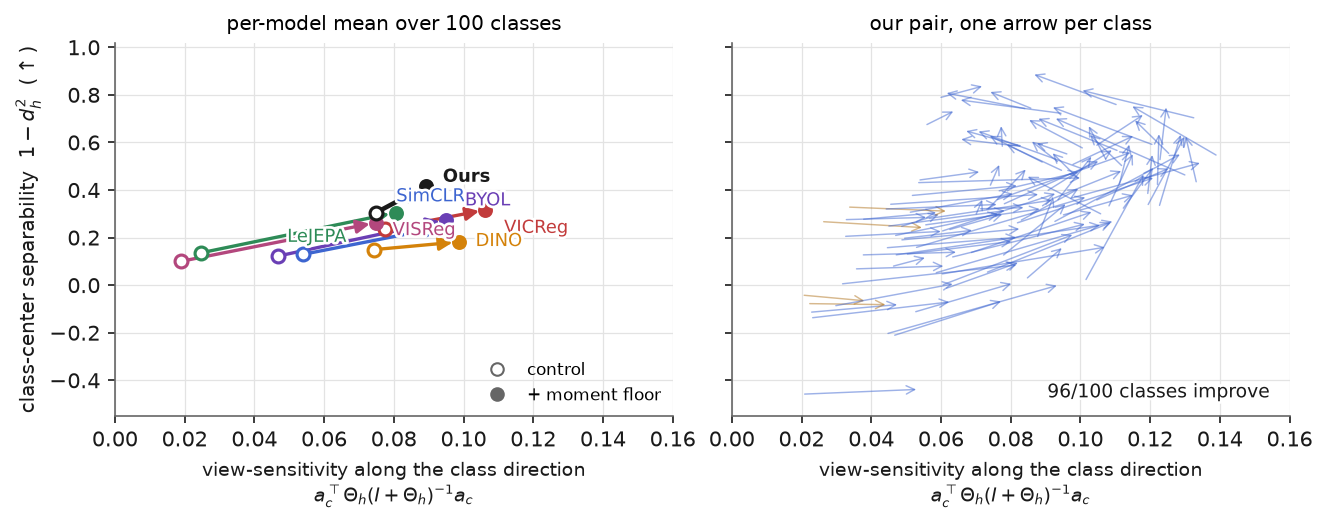
\includegraphics[width=0.85\textwidth]{figures/fig_org_vs_sensitivity.png}
    \caption{
    Image-center organization and view sensitivity along class-prediction directions. Left: average over classes for each method before and after backbone regularization. Right: class-wise changes for our model.
    }
    \label{fig:organization-sensitivity}
\end{figure*}


\section{Conclusion}

\BD{TODO}

% See Appendix. \ref{app:related_works}

% \textbf{SSL.} 


% \textbf{Non-Collapse.} 
% I would introduce it here in my opinion
% \clearpage
% \section{Feature learning inspiered regularizer}
% \label{sec:theory}
% {\color{blue} Please concider this is a draft }
% \label{sec:linear-regulariser}

% Neural networks are typically trained in overparameterised settings, where
% many parameter configurations can realise the same training predictions.
% The optimisation procedure therefore plays an important role in selecting
% among these solutions. Even without explicit regularisation,
% gradient-based optimisation can systematically favour solutions with
% particular geometric or statistical properties, a phenomenon known as
% \emph{implicit regularisation}~\citep{soudry2018implicit}.

% A central distinction in this literature is between lazy and rich learning.
% In the \emph{lazy regime}, the parameters remain close to their
% initialisation and the network is well approximated by its first-order
% linearisation~\citep{chizat2019lazy}. The dynamics then resemble kernel
% regression with an approximately fixed Neural Tangent Kernel
% \citep{jacot2018neural,du2018gradient,du2019gradient,
% allen2019learning,allen2019convergence,zou2020gradient}. In the
% \emph{rich}, or feature-learning, regime, the hidden representations evolve
% in a task-dependent manner and the NTK changes substantially during
% training. In analytically tractable models, these dynamics may proceed
% through a sequence of sigmoidal transitions associated with movement
% between saddle points
% \citep{baldi1989neural,saxe2013exact,saxe2019mathematical,
% jacot2021saddle}. Rich learning has also been connected to low-rank and
% sparse implicit biases
% \citep{li2020towards,woodworth2020kernel,gunasekar2018characterizing,
% savarese2019infinite,lyu2019Gradient,nacson2019lexicographic,
% chizat2020implicit,atanasov_2021_neural}.

% The learning regime depends on both the overall parameter scale and its
% distribution across layers. Small initialisations often promote feature
% learning, whereas appropriate large-scale limits produce kernel-like
% dynamics
% \citep{chizat2019lazy,geiger_2020_disentangling,
% atanasov_2021_neural}. Recent work has shown that the relative scale of
% adjacent layers provides an additional control parameter: asymmetric
% initialisations can qualitatively alter the rate and extent of feature
% learning
% \citep{azulay2021implicit,kunin_2024_get,domine2024lazy,
% jarvis2025theory}. Depending on which layer dominates, such asymmetry may
% either suppress feature evolution or accelerate entry into a rich learning
% regime. Related effects have also been observed in nonlinear networks
% \citep{anguita2026theory,kumar2023grokking,kunin_2024_get}.

% Deep linear networks provide a particularly useful setting in which to
% study these effects. Although their end-to-end mapping is linear, their
% factorised parameterisation produces nonlinear optimisation dynamics and
% captures several phenomena observed in nonlinear networks
% \citep{baldi1989neural,fukumizu1998effect,saxe2013exact,
% nam2025position}. In two-layer linear networks, the relative layer scale is
% captured by the imbalance $\Delta
% =
% \wb^\top\wb-\wa\wa^\top.$
% A network is $\lambda$-balanced when $\Delta
% =
% \lambda\mathbf{I}_{N_h}.$ Under unregularised gradient flow, this quantity is conserved as shown in \ref{}. Consequently,
% existing analyses of $\lambda$-balanced networks select the balance, and
% therefore the associated learning dynamics, through the initialisation
% \citep{domine2024lazy}. And therefore St

% This leads to the central question of this subsection: can the desired
% layer balance be selected \emph{dynamically} by the training objective,
% rather than fixed at initialisation? We first derive our regulariser in a two-layer linear network, where the
% effect of layerwise regularisation on the learning dynamics can be
% characterised exactly. This analysis serves two purposes: it identifies a
% regulariser that dynamically selects the balance between adjacent layers,
% and it establishes an explicit connection between this balance and the
% prevention of representational collapse and learning regime. Next, we extend the resulting construction
% to nonlinear networks.




%  \section*{Acknowledgments}


\bibliography{iclr2027_conference}
\bibliographystyle{iclr2027_conference}

\appendix

\section{A non-collapse regulariser inspired by the feature-learning literature}
\label{app:theory}
\label{sec:exact_learning_dynamics}

\subsection{Linear Network}\label{app:linnet}

\subsubsection{Problem setup}

Consider a supervised learning problem with training data
$
\left\{
    \left(\mathbf{x}_n,\mathbf{y}_n\right)
\right\}_{n=1}^{P},
\mathbf{x}_n\in\mathbb{R}^{N_i},
\mathbf{y}_n\in\mathbb{R}^{N_o}.
$
Let
$
X=
\begin{bmatrix}
\mathbf{x}_1 & \cdots & \mathbf{x}_P
\end{bmatrix}
\in\mathbb{R}^{N_i\times P},$ and $
Y=
\begin{bmatrix}
\mathbf{y}_1 & \cdots & \mathbf{y}_P
\end{bmatrix}
\in\mathbb{R}^{N_o\times P}.
$
We consider a two-layer linear network
$ \widehat{\mathbf{y}}_n = \wb\wa\mathbf{x}_n,
$
with encoder and decoder matrices
$
\wa\in\mathbb{R}^{N_h\times N_i},
\qquad
\wb\in\mathbb{R}^{N_o\times N_h}.
$
The corresponding end-to-end mapping is
$
M=\wb\wa.
$

The empirical mean-squared error is
\begin{equation}
\mathcal{L}_{\mathrm{task}}(\wa,\wb)
=
\frac{1}{2P}
\left\|
    \wb\wa X-Y
\right\|_F^2.
\label{eq:task-loss}
\end{equation}
%More generally, the results below apply to any differentiable task loss of the form $\mathcal{L}_{\mathrm{task}}(\wa,\wb)=\ell(\wb\wa)$
%that depends on the parameter\\lambdas only through the end-to-end mapping. 
We augment the task loss with equal layerwise weight decay and an
encoder-side negative log-determinant regulariser:
\begin{equation}
\mathcal{J}_{\mathrm{enc}}(\wa,\wb)
=
\ell(\wb\wa)
+
\frac{\lambda_{\mathrm{reg}}}{2}
\left(
    \|\wa\|_F^2+\|\wb\|_F^2
\right)
-
\frac{\gamma}{2}
\log\det\left(\wa\wa^\top\right),
\label{eq:encoder-regularised-objective}
\end{equation}
where
$
\lambda_{\mathrm{reg}}>0 $ and $
\gamma>0.
$
The objective is finite only when \(\wa\) has full row rank. We
therefore assume \(N_h\leq N_i\) and initialize the network such that
$
\wa(0)\wa(0)^\top\succ0.
$

Throughout this section, we consider continuous-time gradient flow,
with time constant \(\tau>0\):
\begin{equation}
\tau\dot{\wa}
=
-\nabla_{\wa}\mathcal{J}_{\mathrm{enc}},
\qquad
\tau\dot{\wb}
=
-\nabla_{\wb}\mathcal{J}_{\mathrm{enc}}.
\label{eq:gradient-flow-definition}
\end{equation}

\begin{definition}[\(\lambda\)-balancedness]
\label{def:lambda-balanced}
Define the layer imbalance matrix by
\begin{equation}
\Delta(\wa,\wb)
=
\wb^\top\wb-\wa\wa^\top
\in\mathbb{R}^{N_h\times N_h}.
\label{eq:imbalance-definition}
\end{equation}
The network is said to be \(\lambda_{\mathrm{bal}}\)-balanced if
$\Delta(\wa,\wb)=\lambda_{\mathrm{bal}}\mathbf{I}_{N_h}.$
The case \(\lambda_{\mathrm{bal}}=0\) corresponds to standard
balancedness.
\end{definition}

\subsubsection{Balance conservation without explicit regularisation}

For completeness we first recall the balance-conservation property of two-layer linear
networks trained without explicit regularisation, also derived in \cite{dominé2024lazyrichexactlearning}.

\begin{lemma}[Conservation of layer imbalance]
\label{lem:unregularised-balance-conservation}
Suppose that the network is trained by gradient flow on a
differentiable loss of the form
$ \mathcal{L}_{\mathrm{task}}(\wa,\wb) = \ell(\wb\wa),$
without weight decay or a log-determinant regulariser. Then
\begin{equation}
\frac{\mathrm{d}}{\mathrm{d}t}
\left(
    \wb^\top\wb-\wa\wa^\top
\right)
=
0.
\label{eq:unregularised-balance-conservation}
\end{equation}
Consequently, if the network is
\(\lambda_{\mathrm{bal}}\)-balanced at initialization, then it remains
\(\lambda_{\mathrm{bal}}\)-balanced throughout gradient-flow training.
\end{lemma}

\begin{proof}
Let
$
G
=
\nabla_M\ell(M)\big|_{M=\wb\wa}.
$
The gradient-flow equations for the unregularised task loss are
\[
\tau\dot{\wa}
=
-\wb^\top G,
\qquad
\tau\dot{\wb}
=
-G\wa^\top.
\]
Therefore,
\begin{align}
\tau\frac{\mathrm{d}}{\mathrm{d}t}
\left(\wb^\top\wb\right)
&=
-\wa G^\top\wb
-\wb^\top G\wa^\top,
\\
\tau\frac{\mathrm{d}}{\mathrm{d}t}
\left(\wa\wa^\top\right)
&=
-\wb^\top G\wa^\top
-\wa G^\top\wb.
\end{align}
The two expressions are identical. Subtracting them proves
\eqref{eq:unregularised-balance-conservation}.
\end{proof}

\begin{remark}[Gradient flow versus gradient descent]
The conservation law in
Lemma~\ref{lem:unregularised-balance-conservation} is exact under
continuous-time gradient flow. For finite-step gradient descent,
additional terms of order \(\eta^2\) generally appear, so exact
conservation need not hold for a nonzero learning rate \(\eta\).
\end{remark}


\subsubsection{Non-Collapse Property of Ballanced Initialization}\label{app:noncollapse}

We first show that a negative layer balance is sufficient to prevent
encoder collapse. Under a positive-definiteness assumption on the input
covariance, it also prevents collapse of the hidden representations.
\begin{lemma}[Non-collapse under negative layer balance]
\label{lem:balanced-non-collapse}
Let $\wa\in\mathbb{R}^{N_h\times N_i}$ and
$\wb\in\mathbb{R}^{N_o\times N_h}$ satisfy
\begin{equation}
\wb^\top\wb-\wa\wa^\top
=
\lambda_{\mathrm{bal}}\mathbf{I}_{N_h},
\qquad \lambda_{\mathrm{bal}}<0.
\label{eq:negative-layer-balance}
\end{equation}
Then
$
\wa\wa^\top
\succeq
-\lambda_{\mathrm{bal}}\mathbf{I}_{N_h}.$
Consequently, $\wa$ has full row rank, with
$\sigma_{\min}(\wa)\geq\sqrt{-\lambda_{\mathrm{bal}}}$.

Furthermore, let
$\bar{\mathbf{x}}=P^{-1}\sum_{n=1}^{P}\mathbf{x}_n$
and suppose that the centred empirical input covariance satisfies $\Sigma_x
=
\frac{1}{P}\sum_{n=1}^{P}
(\mathbf{x}_n-\bar{\mathbf{x}})
(\mathbf{x}_n-\bar{\mathbf{x}})^\top
\succeq
\mu\mathbf{I}_{N_i}
\text{ for some }\mu>0.$
For the hidden representations $\mathbf{z}_n=\wa\mathbf{x}_n$,
let $\bar{\mathbf{z}}=P^{-1}\sum_{n=1}^{P}\mathbf{z}_n$.
Their centred empirical covariance then satisfies
\begin{equation}
\boxed{
\Sigma_z
=
\frac{1}{P}\sum_{n=1}^{P}
(\mathbf{z}_n-\bar{\mathbf{z}})
(\mathbf{z}_n-\bar{\mathbf{z}})^\top
\succeq
-\mu\lambda_{\mathrm{bal}}\mathbf{I}_{N_h}
}.
\label{eq:balanced-representation-non-collapse}
\end{equation}
Thus, the representation covariance is positive definite, preventing
both complete and dimensional collapse.
\end{lemma}

\begin{proof}
Rearranging \eqref{eq:negative-layer-balance} gives
\[
\wa\wa^\top
=
\wb^\top\wb-\lambda_{\mathrm{bal}}\mathbf{I}_{N_h}
\succeq
-\lambda_{\mathrm{bal}}\mathbf{I}_{N_h}
\succ0,
\]
since $\wb^\top\wb\succeq0$ and $\lambda_{\mathrm{bal}}<0$.
This establishes the encoder rank and singular-value bounds.

By linearity, $\bar{\mathbf{z}}=\wa\bar{\mathbf{x}}$, so
$\mathbf{z}_n-\bar{\mathbf{z}}
=\wa(\mathbf{x}_n-\bar{\mathbf{x}})$.
Therefore,
\[
\Sigma_z
=
\wa\Sigma_x\wa^\top
\succeq
\mu\wa\wa^\top
\succeq
-\mu\lambda_{\mathrm{bal}}\mathbf{I}_{N_h}
\succ0,
\]
which proves the representation non-collapse bound.
\end{proof}

\begin{remark}
The representation guarantee requires neither whitened inputs nor
zero-mean training data. It requires a strictly positive lower bound
on the centred input covariance. Without this condition, negative
layer balance still guarantees that the encoder has full row rank,
but does not by itself guarantee a full-rank representation covariance.
\end{remark}

Combining Lemma~\ref{lem:unregularised-balance-conservation} with
Lemma~\ref{lem:balanced-non-collapse}, we conclude that a network
initialised with a negative layer balance retains the corresponding
non-collapse bounds throughout unregularised gradient-flow training.
This guarantee depends on the balance imposed at initialisation.




%\begin{lemma}[Non-collapse under negative layer balance]
%\label{lem:balanced-non-collapse}
%Let $\wa\in\mathbb{R}^{N_h\times N_i}$ and
%$\wb\in\mathbb{R}^{N_o\times N_h}$ satisfy
%\begin{equation}
%\wb^\top\wb-\wa\wa^\top
%=
%\lambda_{\mathrm{bal}}\mathbf{I}_{N_h},
%\qquad \lambda_{\mathrm{bal}}<0.
%\label{eq:negative-layer-balance}
%\end{equation}
%Then $\wa\wa^\top
%\succeq
%-\lambda_{\mathrm{bal}}\mathbf{I}_{N_h}$
%and hence $\wa$ has full row rank, with $\sigma_{\min}(\wa)\geq\sqrt{-\lambda_{\mathrm{bal}}}.$
%Furthermore, let $X\in\mathbb{R}^{N_i\times P}$ be the matrix of
%training inputs and suppose that $\Sigma_x=\frac{1}{P}XX^\top
%\succeq\mu\mathbf{I}_{N_i}
%\qquad\text{for some }\mu>0.$
%Then the hidden representations $Z=\wa X$ satisfy
%\begin{equation}
%\boxed{
%\frac{1}{P}ZZ^\top
%\succeq
%-%\mu\lambda_{\mathrm{bal}}\mathbf{I}_{N_h}
%}.
%\label{eq:balanced-representation-non-collapse}
%\end{equation}
%Thus, the hidden representations have full row rank, preventing both
%complete and dimensional %collapse.
%\end{lemma}

%\begin{proof}
%Rearranging \eqref{eq:negative-layer-balance} gives $
%\wa\wa^\top = \wb^\top\wb-\lambda_{\mathrm{bal}}\mathbf{I}_%{N_h}.$
%Since $\wb^\top\wb\succeq0$ and $\lambda_{\mathrm{bal}}<0$, we obtain
%\[
%\wa\wa^\top
%\succeq
%-\lambda_{\mathrm{bal}}\mathbf{I}_{N_h}
%\succ0,
%\]
%which establishes the encoder rank and singular-value bounds.
%For the hidden representations,
%\[
%\frac{1}{P}ZZ^\top
%=
%\wa\Sigma_x\wa^\top
%\succeq
%\mu\wa\wa^\top
%\succeq
%-%\mu\lambda_{\mathrm{bal}}\mathbf{I}_{N_h}.
%\]
%The final lower bound is strictly positive, proving the claim.
%\end{proof}

%\begin{remark}
%The representation guarantee does not require whitened inputs; it
%requires only a strictly positive lower bound on $\Sigma_x$.
%Here, $\Sigma_x$ denotes the empirical second-moment matrix and
%coincides with the empirical covariance when the inputs are centred.
%Without this assumption, negative layer balance still guarantees that
%the encoder has full row rank, but does not by itself guarantee
%full-rank hidden representations.
%\end{remark}




\subsubsection{Constrained optimisation characterisation}
\label{app:opptimisation}
Lemma~\ref{lem:balanced-non-collapse} identifies negative layer balance
as a sufficient condition for non-collapse. We next show that the
proposed regulariser selects precisely such a balance among factorisations of a fixed end-to-end mapping. The regularizer arises from a constrained minimum-regularisation problem.

\begin{theorem}[constrained
optimisation problem characterisation of the selected balance]
\label{app:thm:encoder-variational-balance}
Fix an end-to-end mapping $
M\in\mathbb{R}^{N_o\times N_i}$, $\gamma > 0$, $\lambda_{\mathrm{reg}}> 0$
and consider
\begin{equation}
\begin{aligned}
\min_{\wa,\wb}\quad&
\frac{\lambda_{\mathrm{reg}}}{2}
\left(
    \|\wa\|_F^2+\|\wb\|_F^2
\right)
-
\frac{\gamma}{2}
\log\det\left(\wa\wa^\top\right)
\\
\text{subject to}\quad&
\wb\wa=M.
\end{aligned}
\label{eq:encoder-constrained-problem}
\end{equation}
Let \((\wa^\star,\wb^\star)\) be a regular constrained minimizer with
\(\wa^\star(\wa^\star)^\top\succ0\). Then
\begin{equation}
\boxed{
(\wb^\star)^\top\wb^\star
-
\wa^\star(\wa^\star)^\top
=
-\frac{\gamma}{\lambda_{\mathrm{reg}}}
\mathbf{I}_{N_h}
}.
\label{eq:encoder-variational-balance}
\end{equation}
\end{theorem}

\begin{proof}
Introduce a Lagrange multiplier
$\Lambda\in\mathbb{R}^{N_o\times N_i}$
for the constraint \(\wb\wa=M\). The Lagrangian is
\begin{equation}
\begin{aligned}
\mathscr{L}(\wa,\wb,\Lambda)
={}&
\frac{\lambda_{\mathrm{reg}}}{2}
\left(
    \|\wa\|_F^2+\|\wb\|_F^2
\right)
-
\frac{\gamma}{2}
\log\det\left(\wa\wa^\top\right)
\\
&+
\left\langle
    \Lambda,\wb\wa-M
\right\rangle_F.
\end{aligned}
\label{eq:encoder-constrained-lagrangian}
\end{equation}
The first-order stationarity conditions are
\begin{align}
\lambda_{\mathrm{reg}}\wa
-
\gamma
\left(\wa\wa^\top\right)^{-1}\wa
+
\wb^\top\Lambda
&=0,
\label{eq:encoder-kkt-wa}
\\
\lambda_{\mathrm{reg}}\wb
+
\Lambda\wa^\top
&=0.
\label{eq:encoder-kkt-wb}
\end{align}
Multiplying \eqref{eq:encoder-kkt-wa} on the right by \(\wa^\top\)
gives
\begin{equation}
\lambda_{\mathrm{reg}}\wa\wa^\top
-
\gamma\mathbf{I}_{N_h}
+
\wb^\top\Lambda\wa^\top
=0.
\label{eq:encoder-kkt-gram-wa}
\end{equation}
Multiplying \eqref{eq:encoder-kkt-wb} on the left by \(\wb^\top\)
gives
\begin{equation}
\lambda_{\mathrm{reg}}\wb^\top\wb
+
\wb^\top\Lambda\wa^\top
=0.
\label{eq:encoder-kkt-gram-wb}
\end{equation}
Eliminating the common multiplier term
\(\wb^\top\Lambda\wa^\top\) yields
$
\lambda_{\mathrm{reg}}
\left(
    \wa\wa^\top-\wb^\top\wb
\right)
=
\gamma\mathbf{I}_{N_h},
$
which is equivalent to
\eqref{eq:encoder-variational-balance}.
\end{proof}

\begin{corollary}[Non-collapse at constrained regulariser minima]
\label{cor:encoder-non-collapse}
Under the assumptions of
Theorem~\ref{app:thm:encoder-variational-balance},
\begin{equation}
\boxed{
\wa^\star(\wa^\star)^\top
\succeq
\frac{\gamma}{\lambda_{\mathrm{reg}}}
\mathbf{I}_{N_h}
}.
\label{eq:encoder-anti-collapse-bound}
\end{equation}
Consequently, the encoder has full row rank, with
$\sigma_{\min}(\wa^\star)
\geq
\sqrt{\frac{\gamma}{\lambda_{\mathrm{reg}}}}.$

If, in addition, the centred empirical input covariance $\Sigma_x$
defined in Lemma~\ref{lem:balanced-non-collapse} satisfies
$\Sigma_x\succeq\mu\mathbf{I}_{N_i}$ for some $\mu>0$,
then the centred empirical covariance of the hidden representations
$\mathbf{z}_n^\star=\wa^\star\mathbf{x}_n$ satisfies
\begin{equation}
\boxed{
\Sigma_z^\star
=
\wa^\star\Sigma_x(\wa^\star)^\top
\succeq
\mu\frac{\gamma}{\lambda_{\mathrm{reg}}}
\mathbf{I}_{N_h}
}.
\label{eq:representation-anti-collapse-bound}
\end{equation}
Thus, the representation covariance is positive definite, preventing
both complete and dimensional collapse.
\end{corollary}

\begin{proof}
Theorem~\ref{app:thm:encoder-variational-balance} gives
\[
(\wb^\star)^\top\wb^\star
-
\wa^\star(\wa^\star)^\top
=
-\frac{\gamma}{\lambda_{\mathrm{reg}}}
\mathbf{I}_{N_h}.
\]
Since $\gamma>0$ and $\lambda_{\mathrm{reg}}>0$, this is a
negative layer balance. Both bounds therefore follow directly from
Lemma~\ref{lem:balanced-non-collapse} with
$\lambda_{\mathrm{bal}}=-\gamma/\lambda_{\mathrm{reg}}<0$.
\end{proof}




\subsubsection{Balance selected by the encoder-side regulariser}\label{app:balsel}


For arbitrary $\Delta$, the regularizer exponentially drives the network toward the selected balance. 



\begin{theorem}[Global existence and exponential convergence of layer balance]
\label{thm:encoder-balance-dynamics}
Consider gradient flow with time scale $\tau>0$ on the regularised
mean-squared-error objective
\eqref{eq:encoder-regularised-objective}, with
$\lambda_{\mathrm{reg}}>0$ and $\gamma>0$.
If $\wa(0)\wa(0)^\top\succ0$, then the solution exists for all
$t\geq0$ and the encoder remains full row rank.

Define
\[
\Delta(t)=\wb(t)^\top\wb(t)-\wa(t)\wa(t)^\top,
\qquad
\Delta_\star
=
-\frac{\gamma}{\lambda_{\mathrm{reg}}}\mathbf{I}_{N_h}.
\]
The imbalance satisfies
\[
\tau\dot{\Delta}(t)
=
-2\lambda_{\mathrm{reg}}\bigl(\Delta(t)-\Delta_\star\bigr),
\]
and hence
\begin{equation}
\boxed{
\Delta(t)-\Delta_\star
=
e^{-2\lambda_{\mathrm{reg}}t/\tau}
\bigl(\Delta(0)-\Delta_\star\bigr)
}.
\label{eq:encoder-balance-solution} 
\end{equation}
Thus, for every admissible initialisation, the layer imbalance
converges exponentially to $\Delta_\star$ at rate
$2\lambda_{\mathrm{reg}}/\tau$, selecting the asymptotic balance
$\lambda_{\mathrm{bal}}^{\mathrm{enc}}
=-\gamma/\lambda_{\mathrm{reg}}$.
\end{theorem}

\begin{proof}
We first establish global existence and preservation of encoder
full row rank. Along gradient flow,
\[
\frac{\mathrm{d}}{\mathrm{d}t}\mathcal{J}_{\mathrm{enc}}
=
-\frac{1}{\tau}
\left(
\|\nabla_{\wa}\mathcal{J}_{\mathrm{enc}}\|_F^2
+
\|\nabla_{\wb}\mathcal{J}_{\mathrm{enc}}\|_F^2
\right)
\leq0.
\]
Writing $\sigma_i$ for the encoder singular values, the regulariser is
\[
\mathcal{R}_{\mathrm{enc}}
=
\frac{\lambda_{\mathrm{reg}}}{2}\|\wb\|_F^2
+
\sum_{i=1}^{N_h}
\left(
\frac{\lambda_{\mathrm{reg}}}{2}\sigma_i^2
-\gamma\log\sigma_i
\right).
\]
Each scalar summand is bounded below and diverges at both zero
and infinity. Since the mean-squared-error task loss is nonnegative,
the initial objective sublevel set bounds the weights and keeps
every encoder singular value away from zero. The trajectory thus
remains in a compact subset of the full-row-rank domain, where the
gradient field is smooth. Standard ODE continuation gives global
existence and $\wa(t)\wa(t)^\top\succ0$ for all $t\geq0$.

Now define
\[
G=\nabla_M\ell(M)\big|_{M=\wb\wa},
\qquad
H=\wa\wa^\top.
\]
Since $H\succ0$, it is symmetric and invertible. The gradient of the
encoder-side log-determinant term is
\begin{equation}
\nabla_{\wa}
\left[
-\frac{\gamma}{2}
\log\det\left(\wa\wa^\top\right)
\right]
=
-\gamma H^{-1}\wa.
\label{eq:encoder-logdet-gradient}
\end{equation}
The gradient-flow equations are therefore
\begin{align}
\tau\dot{\wa}
&=
-\wb^\top G
-\lambda_{\mathrm{reg}}\wa
+\gamma H^{-1}\wa,
\label{eq:encoder-wa-flow}
\\
\tau\dot{\wb}
&=
-G\wa^\top
-\lambda_{\mathrm{reg}}\wb.
\label{eq:encoder-wb-flow}
\end{align}

We first compute the dynamics of the decoder Gram matrix.
By the product rule,
\[
\tau\frac{\mathrm{d}}{\mathrm{d}t}
\left(\wb^\top\wb\right)
=
\left(\tau\dot{\wb}\right)^\top\wb
+
\wb^\top\left(\tau\dot{\wb}\right).
\]
Substituting \eqref{eq:encoder-wb-flow} gives
\begin{align}
\tau\frac{\mathrm{d}}{\mathrm{d}t}
\left(\wb^\top\wb\right)
&=
\left(
-G\wa^\top-\lambda_{\mathrm{reg}}\wb
\right)^\top\wb
+
\wb^\top
\left(
-G\wa^\top-\lambda_{\mathrm{reg}}\wb
\right)
\nonumber\\
&=
-\wa G^\top\wb
-\wb^\top G\wa^\top
-2\lambda_{\mathrm{reg}}\wb^\top\wb.
\label{eq:decoder-gram-dynamics}
\end{align}

Similarly, the encoder Gram matrix satisfies
\[
\tau\frac{\mathrm{d}}{\mathrm{d}t}
\left(\wa\wa^\top\right)
=
\left(\tau\dot{\wa}\right)\wa^\top
+
\wa\left(\tau\dot{\wa}\right)^\top.
\]
Substituting \eqref{eq:encoder-wa-flow}, we obtain
\begin{align}
\tau\frac{\mathrm{d}}{\mathrm{d}t}
\left(\wa\wa^\top\right)
={}&
\left(
-\wb^\top G
-\lambda_{\mathrm{reg}}\wa
+\gamma H^{-1}\wa
\right)\wa^\top
\nonumber\\
&+
\wa
\left(
-\wb^\top G
-\lambda_{\mathrm{reg}}\wa
+\gamma H^{-1}\wa
\right)^\top
\nonumber\\
={}&
-\wb^\top G\wa^\top
-\wa G^\top\wb
-2\lambda_{\mathrm{reg}}\wa\wa^\top
\nonumber\\
&+
\gamma H^{-1}\wa\wa^\top
+
\gamma\wa\wa^\top H^{-1}.
\end{align}
Because $H=\wa\wa^\top$, we have
\[
H^{-1}\wa\wa^\top=\mathbf{I}_{N_h},
\qquad
\wa\wa^\top H^{-1}=\mathbf{I}_{N_h}.
\]
Therefore,
\begin{equation}
\tau\frac{\mathrm{d}}{\mathrm{d}t}
\left(\wa\wa^\top\right)
=
-\wb^\top G\wa^\top
-\wa G^\top\wb
-2\lambda_{\mathrm{reg}}\wa\wa^\top
+2\gamma\mathbf{I}_{N_h}.
\label{eq:encoder-gram-dynamics}
\end{equation}

Recall that
\[
\Delta=\wb^\top\wb-\wa\wa^\top.
\]
Subtracting \eqref{eq:encoder-gram-dynamics} from
\eqref{eq:decoder-gram-dynamics} yields
\begin{align}
\tau\dot{\Delta}
={}&
\left(
-\wa G^\top\wb
-\wb^\top G\wa^\top
-2\lambda_{\mathrm{reg}}\wb^\top\wb
\right)
\nonumber\\
&-
\left(
-\wb^\top G\wa^\top
-\wa G^\top\wb
-2\lambda_{\mathrm{reg}}\wa\wa^\top
+2\gamma\mathbf{I}_{N_h}
\right)
\nonumber\\
={}&
-2\lambda_{\mathrm{reg}}
\left(
\wb^\top\wb-\wa\wa^\top
\right)
-2\gamma\mathbf{I}_{N_h}.
\end{align}
The task-loss terms cancel exactly, leaving
\[
\boxed{
\tau\dot{\Delta}
=
-2\lambda_{\mathrm{reg}}\Delta
-2\gamma\mathbf{I}_{N_h}
}.
\]

It remains to solve this linear matrix differential equation.
Dividing by $\tau$ gives
\[
\dot{\Delta}
+
\frac{2\lambda_{\mathrm{reg}}}{\tau}\Delta
=
-\frac{2\gamma}{\tau}\mathbf{I}_{N_h}.
\]
Multiplying both sides by the integrating factor
$e^{2\lambda_{\mathrm{reg}}t/\tau}$ yields
\[
\frac{\mathrm{d}}{\mathrm{d}t}
\left[
e^{2\lambda_{\mathrm{reg}}t/\tau}\Delta(t)
\right]
=
-\frac{2\gamma}{\tau}
e^{2\lambda_{\mathrm{reg}}t/\tau}
\mathbf{I}_{N_h}.
\]
Integrating from $0$ to $t$, we obtain
\begin{align*}
e^{2\lambda_{\mathrm{reg}}t/\tau}\Delta(t)-\Delta(0)
&=
-\frac{2\gamma}{\tau}
\int_0^t
e^{2\lambda_{\mathrm{reg}}s/\tau}
\,\mathrm{d}s\,
\mathbf{I}_{N_h}
\\
&=
-\frac{\gamma}{\lambda_{\mathrm{reg}}}
\left(
e^{2\lambda_{\mathrm{reg}}t/\tau}-1
\right)
\mathbf{I}_{N_h}.
\end{align*}
Multiplying by $e^{-2\lambda_{\mathrm{reg}}t/\tau}$ gives
\[
\Delta(t)
=
e^{-2\lambda_{\mathrm{reg}}t/\tau}\Delta(0)
-
\frac{\gamma}{\lambda_{\mathrm{reg}}}
\left(
1-e^{-2\lambda_{\mathrm{reg}}t/\tau}
\right)
\mathbf{I}_{N_h}.
\]
Equivalently, defining
$\Delta_\star=-(\gamma/\lambda_{\mathrm{reg}})\mathbf{I}_{N_h}$,
\[
\boxed{
\Delta(t)-\Delta_\star
=
e^{-2\lambda_{\mathrm{reg}}t/\tau}
\bigl(\Delta(0)-\Delta_\star\bigr)
}.
\]
Since $\lambda_{\mathrm{reg}}>0$ and $\tau>0$, the imbalance
converges exponentially to $\Delta_\star$ at rate
$2\lambda_{\mathrm{reg}}/\tau$.
No balancedness assumption on $\Delta(0)$ is required.
\end{proof}

\begin{corollary}[Persistence of the selected balance]
\label{cor:selected-balance-persistence}
If the network is initialized such that
$
\Delta(0)
=
-\frac{\gamma}{\lambda_{\mathrm{reg}}}
\mathbf{I}_{N_h},
$
then
$
\Delta(t)
=
-\frac{\gamma}{\lambda_{\mathrm{reg}}}
\mathbf{I}_{N_h}
$
for all \(t\geq0\). Thus, the balance condition selected by the
regulariser is invariant under the regularised gradient-flow dynamics.
\end{corollary}

\begin{proof}
Substituting the assumed initial condition into
\eqref{eq:encoder-balance-solution} gives the result immediately.
\end{proof}


\subsubsection{Rich and Lazy Regime}
\label{app:rich_lazy}


The ratio $\gamma/\lambda_{\mathrm{reg}}$ determines the selected layer balance and thereby influences the learning regime. For a fixed end-to-end mapping, it governs how each singular mode is distributed between the encoder and decoder. Zero balance ($\lambda_{\mathrm{bal}}=0$) corresponds to equal layer singular values, whereas nonzero balance introduces an asymmetry. The effect of this balance on learning depends on the architecture, initialisation scale, and sign of $\lambda_{\mathrm{bal}}$~\citep{dominé2024lazyrichexactlearning}. In the linear setting considered here, sufficiently strong negative imbalance can favour lazy dynamics while preserving the anti-collapse guarantee. By contrast, zero-balanced initialisation can support rich dynamics at sufficiently small initialisation scales. The relationship between imbalance and learning regime is more complex in nonlinear networks, where imbalance is not conserved and does not necessarily induce lazy learning. Appropriate asymmetric parameter scalings can instead accelerate the onset of rich feature-learning dynamics while preserving the non-colapse property. ~\citep{anguita2026theory,kumar2023grokking,kunin_2024_get}. We discuss this distinction further in Appendix~\ref{app:rich_lazy_non}.



%\begin{proposition}[Singular-mode allocation]
%\label{prop:encoder-singular-mode-allocation}
%Assume $N_h\leq\min\{N_i,N_o\},
%$
%and let
%$
%M=USV^\top
%$. Let $
%S=\operatorname{diag}(s_1,\ldots,s_{N_h}),
%$ where $
%s_i\geq0,
%$
%is an \(N_h\)-mode singular value decomposition, padded with zero
%singular values when \(\operatorname{rank}(M)<N_h\). Define
%$
%c
%=
%\frac{\gamma}{\lambda_{\mathrm{reg}}}.
%$
%Up to an orthogonal transformation \(R\in\mathbb{R}^{N_h\times N_h}\)
%of the hidden layer and rotations within degenerate singular
%subspaces, a minimizer of \eqref{eq:encoder-constrained-%problem} can be
%written as
%\begin{equation}
%\wa^\star
%=
%RAV^\top,
%\qquad
%\wb^\star
%=
%UBR^\top,
%\label{eq:encoder-aligned-factors}
%\end{equation}
%where
%$
%A=\operatorname{diag}(a_1,\ldots,a_{N_h}),
%$ and $
%B=\operatorname{diag}(b_1,\ldots,b_{N_h}),
%$
%and
%\begin{align}
%a_i^2
%&=
%\frac{c+\sqrt{c^2+4s_i^2}}{2},
%\label{eq:encoder-ai-explicit}
%\\
%b_i^2
%&=
%\frac{-c+\sqrt{c^2+4s_i^2}}{2}.
\label{eq:encoder-bi-explicit}
%\end{align}
%In particular,
%$
%a_i b_i=s_i,
%$ and $
%a_i^2-b_i^2=c.
%$
%\end{proposition}

%\begin{proof}
%By Theorem~\ref{thm:encoder-variational-balance},
%$
%\wa^\star(\wa^\star)^\top
%-
%(\wb^\star)^\top\wb^\star
%=
%c\mathbf{I}_{N_h}.
%$
%The two Gram matrices therefore commute and share an orthogonal
%eigenbasis \(R\). Consequently, the factors admit the aligned
%representation \eqref{eq:encoder-aligned-factors}, with
%$
%A^2-B^2=c\mathbf{I}_{N_h}.
%$
%The product constraint gives
%$
%\wb^\star\wa^\star
%=
%UBA V^\top
%=
%USV^\top,
%$
%and hence
%$
%BA=S.
%$
%For each singular direction \(i\), we therefore have
%$
%a_i b_i=s_i,
%$ $
%a_i^2-b_i^2=c.
%$
%Setting \(x_i=b_i^2\) gives
%$
%x_i(x_i+c)=s_i^2.
%$
%The nonnegative solution is
%$
%b_i^2
%=
%\frac{-c+\sqrt{c^2+4s_i^2}}{2},
%$
%and adding \(c\) gives
%$
%a_i^2
%=
%\frac{c+\sqrt{c^2+4s_i^2}}{2}.
%$
%\end{proof}

\cite{dominé2024lazyrichexactlearning}

By controlling the ratio $\gamma/\lambda_{\mathrm{reg}}$ (relative scale of the encoder and decoder),the regulariser controls how each end-to-end singular mode is distributed between the two layers and, consequently,  The zero-balanced case,$\lambda_{\mathrm{bal}}=0$, corresponds to symmetric layer scales, whereas a non-zero value produces asymmetric dynamics. 
The regularise further conrols how strongly each layer evolves during training and therefore the learning regime. Previous work has shown that such asymmetry can substantially alter feature learning, with its effect depending on architecture and the sign of $\lambda_{\mathrm{bal}}$ ~\citep{dominé2024lazyrichexactlearning}.In other  in our setting lambda, leads to a lazy regime with an antocolaspse property whilelambda= 0 lead to a rihc regime. 

Related results in nonlinear networks further show that imballanced plays a role, but its effect is different (meaning imballanced doe snot lead to layz ) . It shows that appropriate asymmetric parameter scalings can accelerate the onset of rich feature-learning dynamics~\citep{anguita2026theory,kumar2023grokking,kunin_2024_get}. We further discuss the rich and lazy learning regimes in nonlinear networks (see \ref{app:Two-layer}).




\subsubsection{Experimental verification}
We empirically verify Theorem~\ref{thm:encoder-variational-balance} (and its
dynamical counterpart, Theorem~\ref{thm:encoder-balance-dynamics}) in a
minimal two-layer linear network with no architectural bottleneck,
$N_i=N_h=N_o=8$, so that $W_1,W_2\in\mathbb{R}^{8\times8}$ are both square
and (generically) invertible.

\emph{Task.} Inputs are an orthogonal design $X=\sqrt{N_i}\,I_{N_i}$; targets
$Y$ are a fixed $\{0,\pm1/\sqrt{N_i}\}$-valued matrix with hierarchical block
structure, chosen so that the least-squares solution
$W_{\mathrm{theory}}=\Sigma_{yx}\Sigma_x^{-1}$ has three distinct singular
values (with multiplicities $2,2,4$, reflecting the hierarchy), letting the
predicted balancing effect be checked across multiple directions at once.

\emph{Training protocol.} Both layers are initialised with unbalanced i.i.d.\
Gaussian weights, $W_1(0),W_2(0)\sim\mathcal N(0,\sigma^2)$, $\sigma=0.5$, and
trained by full-batch gradient descent on
$\mathcal{L}_{\mathrm{reg}}=\mathcal{L}_{\mathrm{task}}+\mathcal{R}_{\mathrm{enc}}$
($\eta=10^{-3}$, $T=3\times10^4$ steps), with the log-determinant term on the
\emph{encoder} Gram matrix, $\lambda_{\det}\log\det(W_1)$, and weight decay
$\lambda_{L2}$ on both layers, at $(\lambda_{L2},\lambda_{\det})=(0.1,-0.2)$ —
the cell shown in Figure~\ref{appfig:linearreg}.

\emph{Verification protocol.} At $t=T$ we compare three block Gram matrices
$Q=\begin{pmatrix}W_1^\top W_1 & W^\top\\ W & W_2W_2^\top\end{pmatrix}$,
$W=W_2W_1$: \textbf{(A)} $Q_{\mathrm{emp}}$ from the regularised network;
\textbf{(B)} $Q_{\mathrm{theory}}$, obtained by reassigning the singular
values of $W_{\mathrm{theory}}$ to the two layers via
$S_1^2=S_\lambda-\lambda_{\mathrm{bal}}/2$,
$S_2^2=S_\lambda+\lambda_{\mathrm{bal}}/2$
(Section~\ref{app:singular}), with
$\lambda_{\mathrm{bal}}=\lambda_{\det}/\lambda_{L2}=-2$; and \textbf{(C)}
$Q_{\mathrm{bal}}$, from a network initialised exactly at this
$\lambda_{\mathrm{bal}}$-balanced solution and trained unregularised
($\lambda_{L2}=\lambda_{\det}=0$), whose balance is conserved by construction
under unregularised gradient flow.

Figure~\ref{appfig:linearreg} shows near-perfect agreement across all
three panels. The empirical imbalance eigenvalues concentrate tightly around
the predicted, negative fixed point,
$\mathrm{eig}(\Lambda(T))\in[-2.005,-1.984]\approx\lambda_{\mathrm{bal}}I$, and
the small relative error,
\[
\varepsilon
=
\frac{\lVert Q_{\mathrm{emp}} - Q_{\mathrm{theory}} \rVert_F}
{\lVert Q_{\mathrm{theory}} \rVert_F}
=
0.0095,
\]
confirms that the encoder-side log-determinant regulariser drives the
network towards the predicted, collapse-preventing balanced fixed point,
without impeding task fit (final MSE $\approx5.47\times10^{-4}$).


\begin{figure}
\begin{center}
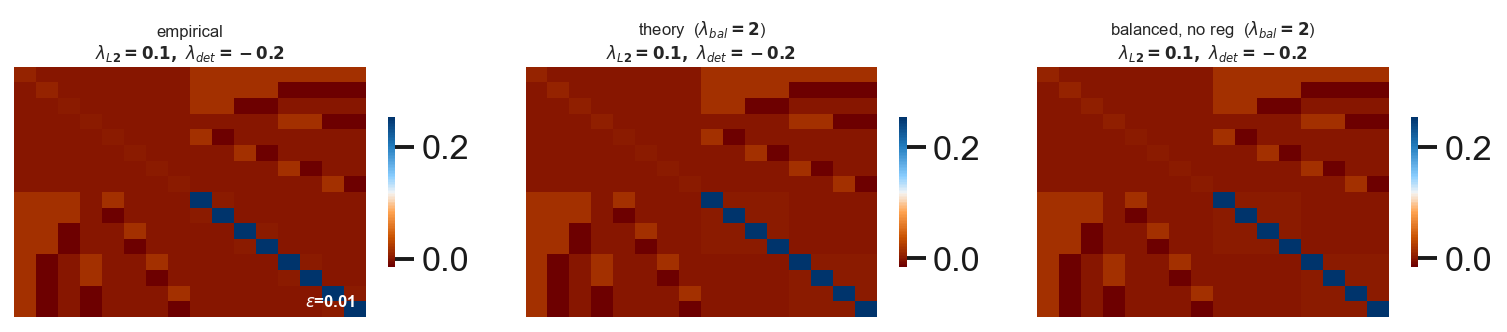
\includegraphics[width=0.9\textwidth]{./figures/linear_figure.png}
\end{center}
\caption{
Block Gram matrix
$
Q=
\begin{pmatrix}
\wa^\top\wa & M^\top\\
M & \wb\wb^\top
\end{pmatrix},
\qquad M=\wb\wa,
$
for a two-layer linear network.
\textbf{(A)} Training with symmetric $L_2$ weight decay
($\lambda_{\mathrm{reg}}=0.1$) and an encoder-side
negative log-determinant penalty ($\gamma=0.2$).
The regulariser drives the layer imbalance
$\Delta=\wb^\top\wb-\wa\wa^\top$
towards
$\Delta_\star=-(\gamma/\lambda_{\mathrm{reg}})
\mathbf{I}_{N_h}=-2\mathbf{I}_{N_h}$,
corresponding to $\lambda_{\mathrm{bal}}=-2$.
\textbf{(B)} Closed-form prediction from
Appendix~\ref{app:singular}.
\textbf{(C)} Unregularised control network initialised at
$\lambda_{\mathrm{bal}}=-2$.
This balance is conserved under gradient flow, providing a
comparison with the balance selected dynamically in~(A).
}
\label{appfig:linearreg}
\end{figure}






\subsection{From linear to nonlinear covariance regularisation}


\subsubsection{From linear balance to nonlinear covariance regularisation}
\label{sec:nonlinear-covariance-regularisation}

%The preceding linear analysis shows that constrained minimisers of
%the encoder-side regulariser satisfy
%\[
%\\wb^\top\wb-\wa\wa^\top
%\=
%\-\frac{\gamma}{\lambda_{\mathrm{reg}}}\mathbf{I}_{N_h},
%\\]
%\and therefore
%\\[
%\\wa\wa^\top
%\\succeq
%\\frac{\gamma}{\lambda_{\mathrm{reg}}}\mathbf{I}_{N_h}.
%\\]
%\Regularised gradient flow also converges towards this selected
%\balance. 

%These results motivate applying the same spectral
%regularisation directly to the covariance of nonlinear
%representations. We additionally penalise the representation mean,
%which need not vanish even when the inputs are centred.

For a linear encoder with centred, whitened inputs and $\varepsilon=0$, the covariance penalty reduces exactly to the encoder portion of the linear regulariser, with $\lambda_{\mathrm{cov}}=\lambda_{\mathrm{reg}}$. 

\begin{lemma}[Linear encoder mean and covariance]
\label{lem:linear-gram-covariance}
Let $x\in\mathbb{R}^{N_i}$ have finite second moments, mean
$\mu_x=\mathbb{E}[x]$, and covariance
$\Sigma_x=\mathbb{E}[(x-\mu_x)(x-\mu_x)^\top]$.
For the bias-free linear representation $z=\wa x$, its mean
and covariance satisfy $\mu_z=\wa\mu_x, $
\text{}$
C_z=\wa\Sigma_x\wa^\top.$

In particular, for centred, whitened inputs,
$\mu_x=0$ and $\Sigma_x=\mathbf{I}_{N_i}$, so $\mu_z=0,
\qquad
C_z=\wa\wa^\top,
\qquad
\operatorname{tr}(C_z)=\|\wa\|_F^2.$
\end{lemma}

\begin{proof}
By linearity of expectation, $\mu_z=\mathbb{E}[\wa x]=\wa\mu_x.$
Consequently, $z-\mu_z=\wa(x-\mu_x)$, giving $C_z
=
\mathbb{E}[(z-\mu_z)(z-\mu_z)^\top]
=
\wa\Sigma_x\wa^\top.$
For centred, whitened inputs, these identities reduce to
$\mu_z=0$ and $C_z=\wa\wa^\top$. Taking the trace yields
$\operatorname{tr}(C_z)=\|\wa\|_F^2$.
\end{proof}

\paragraph{Recovery of the linear encoder regulariser.}
Recall that the nonlinear regulariser is
\[
\mathcal{R}_{\mathrm{SAC}}(\mu_z,C_z)
=
\frac{\lambda_{\mathrm{mean}}}{2}\|\mu_z\|_2^2
+
\frac{\lambda_{\mathrm{cov}}}{2}\operatorname{tr}(C_z)
-
\frac{\gamma}{2}
\log\det(C_z+\varepsilon\mathbf{I}_{N_h}).
\]
Assume $\wa\wa^\top\succ0$, centred and whitened inputs,
$\varepsilon=0$, and
$\lambda_{\mathrm{cov}}=\lambda_{\mathrm{reg}}$.
Lemma~\ref{lem:linear-gram-covariance} then gives
\[
\mathcal{R}_{\mathrm{SAC}}(\mu_z,C_z)
=
\frac{\lambda_{\mathrm{reg}}}{2}\|\wa\|_F^2
-
\frac{\gamma}{2}\log\det(\wa\wa^\top).
\]
The mean penalty vanishes because $\mu_z=0$, regardless of the
positive value of $\lambda_{\mathrm{mean}}$.
Thus, the nonlinear regulariser reduces exactly to the encoder
portion of the linear regulariser:
\[
\mathcal{R}_{\mathrm{enc}}(\wa,\wb)
=
\mathcal{R}_{\mathrm{SAC}}(\mu_z,C_z)
+
\frac{\lambda_{\mathrm{reg}}}{2}\|\wb\|_F^2.
\]

\paragraph{Role of the mean penalty.}
For nonlinear encoders, centred inputs need not produce centred
representations. Moreover, covariance is invariant under a common
translation of all representations, so neither the trace nor the
log-determinant term controls their mean. The additional
$\|\mu_z\|_2^2$ penalty controls this translation by favouring
zero-mean representations. It therefore extends the regulariser
without changing its reduction to the bias-free linear setting
with centred, whitened inputs.The same identities hold for empirical means and covariances.



\subsubsection{Log-determinant covariance regulariser with the mean }
\label{sec:logdet-covariance-regulariser}

Let $z=f_\theta(x)\in\mathbb{R}^{k}$ denote the representation produced by a possibly nonlinear
encoder. For a minibatch of size \(B\), collect the representations row-wise in $Z=\in\mathbb{R}^{B\times k}.$
Define the empirical mean, centering matrix, centered representations, and empirical covariance
$
\mu=\frac{1}{B}Z^\top\mathbf{1},
$ $
P_B
=
I_B-\frac{1}{B}\mathbf{1}\mathbf{1}^\top,
$ $
\widetilde Z=P_BZ,
$ $
C_z
=
\frac{1}{B}\widetilde Z^\top\widetilde Z
\succeq0.$ The linear analysis never needs to control the
representation's mean: for a bias-free linear encoder $z=\wa x$ with centered input, $\mathbb
E[z]=\wa\,\mathbb E[x]=0$ identically, so the mean carries no independent degree of freedom for
$\mathcal R_{\mathrm{enc}}$ to regularise. This guarantee does not survive the transfer to a
general nonlinear (or biased) encoder: a bias term, or the nonlinearity itself (e.g.\ a ReLU
clipping one side of an otherwise symmetric pre-activation), can give $z$ a nonzero mean that
moves independently of $C_z$ -- invisible to both $\operatorname{tr}(C_z)$ and $\log\det(C_z)$,
since $C_z$ is computed from the \emph{centered} representation by construction. We therefore
regularise $\mu$ directly alongside $C_z$. Motivated by the linear encoder regulariser, we define

\begin{definition}[Nonlinear SACReg]
\label{def:nonlinear-encoder-regulariser}
Let $\lambda_{\mathrm{mean}}>0$,
$\lambda_{\mathrm{cov}}>0$, $\gamma>0$, and $\varepsilon\geq0$.
Assume that $C_z+\varepsilon\mathbf{I}_k\succ0$.
We define
\begin{equation}
\mathcal{R}_{\mathrm{SAC}}(\mu,C_z)
=
\frac{\lambda_{\mathrm{mean}}}{2}\|\mu\|_2^2
+
\frac{\lambda_{\mathrm{cov}}}{2}\operatorname{tr}(C_z)
-
\frac{\gamma}{2}
\log\det\left(C_z+\varepsilon\mathbf{I}_k\right).
\label{eq:nonlinear-covariance-regulariser}
\end{equation}
\end{definition}
 The mean term controls the representation's location, the trace term controls its overall scale, and
the negative log-determinant penalizes small covariance eigenvalues.


To understand the inductive bias of the regulariser, we consider its minimizer in isolation. This does not imply that the mean and covariance of the complete learning objective must attain this value, since the task loss may introduce competing constraints First, we write the regularizer in spectral form.


\begin{proposition}[Spectral form]
\label{prop:nonlinear-covariance-spectral-form}
Let $\lambda_1(C_z),\ldots,\lambda_k(C_z)$ be the eigenvalues of \(C_z\). Then
\begin{equation}
\mathcal{R}_{\mathrm{SAC}}(\mu,C_z)
=
\frac{\lambda_{\mathrm{mean}}}{2}\|\mu\|^2
+
\frac{1}{2}
\sum_{i=1}^{k}
\left[
    \lambda_{\mathrm{cov}}\lambda_i(C_z)
    -
    \gamma\log\left(
        \lambda_i(C_z)+\varepsilon
    \right)
\right].
\label{eq:nonlinear-covariance-eigenvalue-form}
\end{equation}
\end{proposition}
\begin{proof}
Because \(C_z\) is symmetric and positive semidefinite, it admits an eigendecomposition
$C_z=Q\operatorname{diag}(\lambda_1,\ldots,\lambda_k)Q^\top$. Consequently,
$\operatorname{tr}(C_z)=\sum_{i=1}^{k}\lambda_i$ and $\log\det(C_z+\varepsilon I_k)
=\sum_{i=1}^{k}\log(\lambda_i+\varepsilon)$. The mean term does not depend on $C_z$. Substitution
into \eqref{eq:nonlinear-covariance-regulariser} proves the result.
\end{proof}

We can now write the optimal mean and covariance.

\begin{theorem}[Optimal mean and covariance]
\label{thm:nonlinear-optimal-covariance}
The unique minimizer of \(\mathcal{R}_{\mathrm{SAC}}\) over $\mu\in\mathbb R^k,\ C_z\succeq0$ is
\begin{equation}
\boxed{
\mu^\star=0,
\qquad
C_z^\star
=
\left(
    \frac{\gamma}{\lambda_{\mathrm{cov}}}
    -
    \varepsilon
\right)_{+}I_k
},
\label{eq:nonlinear-optimal-covariance}
\end{equation}
where $(a)_{+}=\max\{a,0\}$. Therefore, the covariance-level optimum is full-rank if and only if
$\gamma>\lambda_{\mathrm{cov}}\varepsilon$, independently of $\mu^\star$.
\end{theorem}

\begin{proof}
By Proposition~\ref{prop:nonlinear-covariance-spectral-form}, $\mathcal{R}_{\mathrm{SAC}}$ is a sum
of a term depending only on $\mu$ and a term depending only on $C_z$, so the two may be minimized
separately. The mean term $\frac{\lambda_{\mathrm{mean}}}{2}\|\mu\|^2$ is uniquely minimized at
$\mu^\star=0$. For the covariance term, each eigenvalue independently minimizes the strictly
convex function
\[
\phi(s)
=
\frac{\lambda_{\mathrm{cov}}}{2}s
-
\frac{\gamma}{2}\log(s+\varepsilon),
\qquad
s\geq0.
\]
Its derivatives are $\phi'(s)=\frac{\lambda_{\mathrm{cov}}}{2}-\frac{\gamma}{2(s+\varepsilon)}$ and
$\phi''(s)=\frac{\gamma}{2(s+\varepsilon)^2}>0$. The unconstrained stationary point satisfies
$\phi'(s)=0 \Leftrightarrow s=\frac{\gamma}{\lambda_{\mathrm{cov}}}-\varepsilon$. If this value is
positive, it is the unique minimizer; otherwise the minimum over $s\geq0$ occurs at $s=0$.
Applying this argument to every covariance eigenvalue proves
\eqref{eq:nonlinear-optimal-covariance}.
\end{proof}

\begin{corollary}[Isotropic non-collapsed target, centered]
\label{cor:nonlinear-isotropic-target}
In the idealized case \(\varepsilon=0\),
\begin{equation}
\boxed{
\mu^\star=0,
\qquad
C_z^\star
=
\frac{\gamma}{\lambda_{\mathrm{cov}}}I_k
}.
\label{eq:nonlinear-isotropic-covariance}
\end{equation}
Thus, the regularizer simultaneously:
\begin{enumerate}
    \item centers the representation at the origin;
    \item prevents the covariance eigenvalues from vanishing;
    \item equalizes the covariance spectrum;
    \item controls the overall representation scale; and
    \item selects a condition number equal to one.
\end{enumerate}

\end{corollary}

{\color{blue}

Next we derive the non-collapse property of the regularizer.
 
\begin{theorem}[Strict mean and covariance non-collapse]
\label{thm:strict-covariance-non-collapse}
Suppose that \(\varepsilon=0\). Then
\begin{equation}
\lambda_{\min}(C_z)\to0
\quad\Longrightarrow\quad
\mathcal{R}_{\mathrm{SAC}}(\mu,C_z)\to+\infty,
\label{eq:covariance-collapse-barrier}
\end{equation}
\begin{equation}
\lambda_{\max}(C_z)\to+\infty
\quad\Longrightarrow\quad
\mathcal{R}_{\mathrm{SAC}}(\mu,C_z)\to+\infty,
\label{eq:covariance-scale-barrier}
\end{equation}
\begin{equation}
\|\mu\|\to\infty
\quad\Longrightarrow\quad
\mathcal{R}_{\mathrm{SAC}}(\mu,C_z)\to+\infty.
\label{eq:mean-blowup-barrier}
\end{equation}
Consequently, every finite sublevel set of \(\mathcal{R}_{\mathrm{SAC}}\) is jointly bounded away
from covariance collapse, covariance blowup, and mean blowup: for every finite \(K\), there exist
constants $0<m_K\leq M_K<\infty$ and $M'_K<\infty$ such that
\begin{equation}
\mathcal{R}_{\mathrm{SAC}}(\mu,C_z)\leq K
\quad\Longrightarrow\quad
m_KI_k
\preceq
C_z
\preceq
M_KI_k
\ \text{ and }\ \|\mu\|^2\leq M'_K.
\label{eq:covariance-spectral-sublevel-bound}
\end{equation}
\end{theorem}

\begin{proof}
Suppose that \(\varepsilon=0\) and \(C_z\succ0\). Let $\lambda_1(C_z),\ldots,\lambda_k(C_z)>0$
denote the eigenvalues of \(C_z\). Since $\operatorname{tr}(C_z)=\sum_{i=1}^k\lambda_i(C_z)$ and
$\log\det(C_z)=\sum_{i=1}^k\log\lambda_i(C_z)$, write
\[
\mathcal{R}_{\mathrm{SAC}}(\mu,C_z) = \frac{\lambda_{\mathrm{mean}}}{2}\|\mu\|^2+\sum_{i=1}^k
\phi\left(\lambda_i(C_z)\right),
\qquad
\phi(s)
=
\frac{\lambda_{\mathrm{cov}}}{2}s
-
\frac{\gamma}{2}\log s,
\quad
s>0.
\]
We first show that \(\phi\) is bounded below. Its derivatives are
$\phi'(s)=\frac{\lambda_{\mathrm{cov}}}{2}-\frac{\gamma}{2s}$ and
$\phi''(s)=\frac{\gamma}{2s^2}>0$, so \(\phi\) is strictly convex, with unique stationary point
$s=\gamma/\lambda_{\mathrm{cov}}$ and global minimum
\[
b
:=
\min_{s>0}\phi(s)
=
\phi\!\left(\frac{\gamma}{\lambda_{\mathrm{cov}}}\right)
=
\frac{\gamma}{2}
-
\frac{\gamma}{2}
\log\!\left(\frac{\gamma}{\lambda_{\mathrm{cov}}}\right).
\]
In particular, $\phi(s)\geq b$ for every $s>0$, so $\sum_{i=1}^k\phi(\lambda_i(C_z))\geq kb$ for
every $C_z\succ0$.

\emph{Covariance collapse.} Without loss of generality order the eigenvalues so that
$\lambda_1(C_z)=\lambda_{\min}(C_z)$. Then
\[
\mathcal{R}_{\mathrm{SAC}}(\mu,C_z)
\;\geq\;
\phi\left(\lambda_{\min}(C_z)\right)
+
(k-1)b.
\]
As $s\downarrow0$, $\frac{\lambda_{\mathrm{cov}}}{2}s\to0$ and $-\frac{\gamma}{2}\log s\to+\infty$,
so $\lim_{s\downarrow0}\phi(s)=+\infty$. Since $(k-1)b$ is a fixed finite constant,
$\lambda_{\min}(C_z)\to0\Rightarrow\mathcal{R}_{\mathrm{SAC}}(\mu,C_z)\to+\infty$, proving
\eqref{eq:covariance-collapse-barrier}.

\emph{Covariance blowup.} As $s\to+\infty$, $\frac{\lambda_{\mathrm{cov}}}{2}s\to+\infty$ dominates
$-\frac{\gamma}{2}\log s$, so $\phi(s)\to+\infty$; the same argument with $\lambda_{\max}(C_z)$ in
place of $\lambda_{\min}(C_z)$ proves \eqref{eq:covariance-scale-barrier}.

\emph{Mean blowup.} Fixing $C_z$ and letting $\|\mu\|\to\infty$, $\sum_i\phi(\lambda_i(C_z))$ stays
fixed while $\frac{\lambda_{\mathrm{mean}}}{2}\|\mu\|^2\to+\infty$, proving
\eqref{eq:mean-blowup-barrier}.

\emph{Joint sublevel bound.} Suppose $\mathcal{R}_{\mathrm{SAC}}(\mu,C_z)\leq K$. Since
$\frac{\lambda_{\mathrm{mean}}}{2}\|\mu\|^2\geq0$, we get $\sum_i\phi(\lambda_i(C_z))\leq K$, and
the collapse/blowup limits above give constants $0<m_K\leq M_K<\infty$ (depending only on
$K,\lambda_{\mathrm{cov}},\gamma,k$) with $m_KI_k\preceq C_z\preceq M_KI_k$. Since
$\sum_i\phi(\lambda_i(C_z))\geq kb$, we also get
\[
\frac{\lambda_{\mathrm{mean}}}{2}\|\mu\|^2
\leq
K-\sum_i\phi(\lambda_i(C_z))
\leq
K-kb
\;\Longrightarrow\;
\|\mu\|^2\leq\frac{2}{\lambda_{\mathrm{mean}}}(K-kb)=:M'_K,
\]
finite since $K,k,b$ are all finite. This proves \eqref{eq:covariance-spectral-sublevel-bound}.
\end{proof}}



\begin{remark}[Effect of the numerical stabilizer]
The regularizer prevents covariance collapse when \(\varepsilon=0\), but only discourages it when \(\varepsilon>0\). In the latter case, its unique covariance-level minimizer is still full-rank provided \(\gamma>\lambda_{\mathrm{cov}}\varepsilon\) (Theorem~\ref{thm:nonlinear-optimal-covariance}). Mean non-blowup remains guaranteed in both cases.
\end{remark}


\begin{remark}[Scope of the nonlinear extension]
The nonlinear covariance regularizer is motivated by the exact linear balance analysis, but it
does not imply that the linear balance identity $\wb^\top\wb-\wa\wa^\top
=-\frac{\gamma}{\lambda_{\mathrm{reg}}}I$ continues to hold for a general nonlinear encoder. The
nonlinear parameter dynamics are modified by the encoder Jacobian, and there is generally no
conserved difference between the decoder Gram matrix and the representation covariance. 
\end{remark}

x


% =========================
% Rich feature learning
% =========================
\begin{figure*}[h]
    \centering
\includegraphics[width=\textwidth]{figures/Rich.png}
    \caption{Effective rank and kernel distance of the NTK from initialization. \textbf{Top row:} Both metrics as functions of the scale $\tau$ and relative scale $\lambda$ at step $t = 20{,}000$, without regularization ($w_{\mathrm{reg}} = 0$). \textbf{Bottom row:} The same metrics at the final checkpoint as functions of the scale $\tau$ and regularization weight $w_{\mathrm{reg}}$, with $\lambda = 0$ fixed.    }
    \label{fig:rich-Relu}
\end{figure*}



\subsubsection{Feature Learning:Two-layer Relu Experiment}
\label{app:Two-layer}
\paragraph{Task and data.}
We study nonlinear teacher--student regression with a fixed,
untrained two-layer ReLU teacher of hidden width \(m_0=3\).
The teacher is $f_\star(x)
=
\sum_{j=1}^{m_0} a^\star_j
\sigma\!\left((w^\star_j)^\top x\right),
\text{with }
\sigma(z)=\max\{0,z\},$
where \(w^\star_j\) are sampled independently and uniformly from
the unit sphere \(\mathbb{S}^{d-1}\), and \(a^\star_j\) are
independent Rademacher random variables.
For each run, we sample \(n=1{,}000\) training inputs independently
from \(\mathbb{S}^{d-1}\) and assign noiseless labels
\(y_i=f_\star(x_i)\).
A separate test set of \(n_{\mathrm{test}}=10{,}000\) inputs,
generated with seed \(201\), is reused at every checkpoint for
both test-loss and representation-rank measurements.


\paragraph{Student architecture.}
The student is a two-layer, bias-free ReLU network with
hidden width \(m=50\): $h_\theta(x)=\sigma(Wx)\in\mathbb{R}^{m},$ and $f_\theta(x)=a^\top h_\theta(x).$
We measure the rank of the post-ReLU representation
\(h_\theta(x)\), the network's only hidden layer.
The student uses a symmetric initialization: hidden units
form \(m/2\) pairs with identical input weights and
opposite readout weights, $w_{j+m/2}=w_j,
$ $
a_{j+m/2}=-a_j,
\qquad j=1,\ldots,m/2.$ This ensures \(f_{\theta_0}(x)=0\) for every input while retaining a nontrivial initial neural tangent kernel (NTK).

\paragraph{Initialization.}
Two parameters control initialization: an overall scale
\(\tau>0\) and a layer imbalance \(\lambda\).
For each independently sampled pair, we initialize $w_j=\tau\alpha u_j,
\text{ and }
a_j=\frac{\tau}{\alpha}s_j,$
where \(u_j\) is uniform on \(\mathbb{S}^{d-1}\),
\(s_j\in\{-1,+1\}\) is a Rademacher random variable, and
\(\alpha>0\) satisfies $\lambda
=
\tau^2\left(\alpha^2-\alpha^{-2}\right).$
Equivalently, $\alpha
=
\left(
\frac{\lambda/\tau^2+
\sqrt{(\lambda/\tau^2)^2+4}}{2}
\right)^{1/2}.
$
Thus, \(\tau\) controls the overall weight scale, whereas
\(\lambda\) controls the relative magnitudes of the input
and readout weights.


{\color{blue}
\paragraph{Objective and optimization.}
We train the student using full-batch gradient descent on
the mean squared error, $\mathcal{L}_{\mathrm{MSE}}(\theta)
=
\frac{1}{n}\sum_{i=1}^{n}
\left(f_\theta(x_i)-y_i\right)^2,$ with an additional regularisation term in the regularised
experiments. No data augmentation or mini-batching is used.
The learning rate is scaled as $\eta=\frac{5\times10^{-3}}{\tau^2}.$ . Cross-validation of the two implementations showed agreement to three--four significant figures. We apply the log-determinant covariance regulariser directly to the hidden representation of the toy two-layer ReLU student network, $h = \mathrm{ReLU}(W_1 x) \in \mathbb{R}^m$ (here $m=50$), immediately after the nonlinearity and before the readout layer.

At each optimization step, given a batch of $B$ representations ${h_i}{i=1}^{B}$, we draw a fresh random orthonormal matrix $Q \in \mathbb{R}^{m \times d'}$ (via QR decomposition of a matrix with i.i.d. Gaussian entries) and project each representation, $p_i = Q^\top h_i \in \mathbb{R}^{d'}$. We then compute the empirical mean and covariance of the projected batch,
$\mu = \frac{1}{B}\sum{i=1}^{B} p_i, \qquad
\Sigma = \frac{1}{B-1}\sum_{i=1}^{B} (p_i-\mu)(p_i-\mu)^\top,
$
and define the regulariser as
$ \mathcal{R}(h) ;=; \frac{1}{2d'}\Big(\operatorname{tr}(\Sigma+\varepsilon I) + |\mu|^2 - d' - \log\det(\Sigma+\varepsilon I)\Big)$
where $\varepsilon>0$ is a small numerical stabilizer added to the diagonal of $\Sigma$. In the experiments reported here we set $d'=m$ (the projection is a full-dimensional random rotation rather than a dimensionality-reducing slice), $\varepsilon=10^{-4}$, and redraw $Q$ independently at every step.

Here we used $\lambda_{\text{cov}}=\gamma$ 
Therefore, the regularised training objective is $\mathcal{L} ;=; \mathcal{L}{\text{task}} + w{\text{reg}}\cdot \mathcal{R}(h),
$ with $\mathcal{L}{\text{task}}$ the mean-squared error between the student's output and the teacher's labels, and $w{\text{reg}} \in {0,\pm0.001,\pm0.005,\pm0.02,\pm0.1}$ swept as the regulariser strength; negative $w_{\text{reg}}$ reverses the sign of the penalty, rewarding deviation from $\mathcal{N}(0,I)$ rather than penalizing it.
}

\textbf{Feature learning}
Using the two-layer ReLU network setup of \cite{kunin_2021_neural}, investigate how the rank effects  and the learning regime of the initial imbalance $\lambda$ relate to those of the SAC regulariser. Linear theory suggests that a negative relative scale should favour the same anti-collapse behaviour promoted by SAC regularisation.

\begin{itemize}
  
\item \textit{Rank} There is no exact correspondence between the initial imbalance $\lambda$ and the regularisation weight $w_{\mathrm{reg}}$. The regulariser appears to exert a substantially stronger effect on rank (see Fig. \ref{fig:rich-Relu}). Nevertheless, both negative $\lambda$ (relative to $\lambda\geq 0$) and positive $w_{\mathrm{reg}}$ favour higher rank in the Rich regime, supporting a qualitative connection between initial imbalance and anti-collapse regularisation (see Fig. \ref{fig:rich-Relu}). Interestingly, the rank effect of negative $\lambda$ emerges during training rather than reflecting a decaying initial offset. All negative-$\lambda$ runs with $w_{\mathrm{reg}}=0$ begin at approximately the same effective rank fraction, $\mathtt{effrank\_frac}=0.467$, consistent with their shared initialisation (See table \ref{tab:effective-rank}. This quantity then increases monotonically throughout training, indicating that the higher final rank develops through the training dynamics. 
\item \textit{Learning regime.} We characterise the learning regime by measuring the departure of the neural tangent kernel (NTK) from its value at initialisation, quantified by $\mathtt{kernel\_distance}$. Increasing $w_{\mathrm{reg}}$ leads to an increase in kernel distance across the initialisation scales considered, indicating that stronger regularisation promotes greater kernel evolution (see Fig. \ref{fig:rich-Relu}). It also extends the range of initialisation scales over which feature learning occurs, although kernel evolution remains limited at sufficiently large scales (see Fig.~\ref{fig:rich-Relu}). At small initialisation scales, varying $\lambda$ alone yields $\mathtt{kernel\_distance}$ values between $0.16$ and $0.58$, comparable to the range obtained by varying $w_{\mathrm{reg}}$. At large initialisation scales, however, both parameters have little effect on kernel evolution. These results suggest that $\lambda$ primarily modulates the degree of feature learning within an already rich regime, whereas $w_{\mathrm{reg}}$ can also promote departures from otherwise lazy dynamics.
\end{itemize}



\begin{table}[htbp]
\centering
\caption{Effective rank fraction across training steps for different
values of label imbalance $\lambda$.}
\label{tab:effective-rank}
\begin{tabular}{r|rrrrrr}
\hline
 & \multicolumn{6}{c}{Training step} \\
$\lambda$ & $0$ & $100$ & $1000$ & $5000$ & $10000$ & $20000$ \\
\hline
$-1.00$ & 0.467 & 0.467 & 0.484 & 0.554 & 0.574 & 0.581 \\
$-0.75$ & 0.467 & 0.467 & 0.487 & 0.563 & 0.587 & 0.595 \\
$-0.50$ & 0.467 & 0.467 & 0.492 & 0.577 & 0.606 & 0.616 \\
$-0.25$ & 0.467 & 0.469 & 0.500 & 0.596 & 0.627 & 0.639 \\
\hline
\end{tabular}
\end{table}

% =========================
% Rich feature learning
% =========================
\begin{figure*}[h]
    \centering
    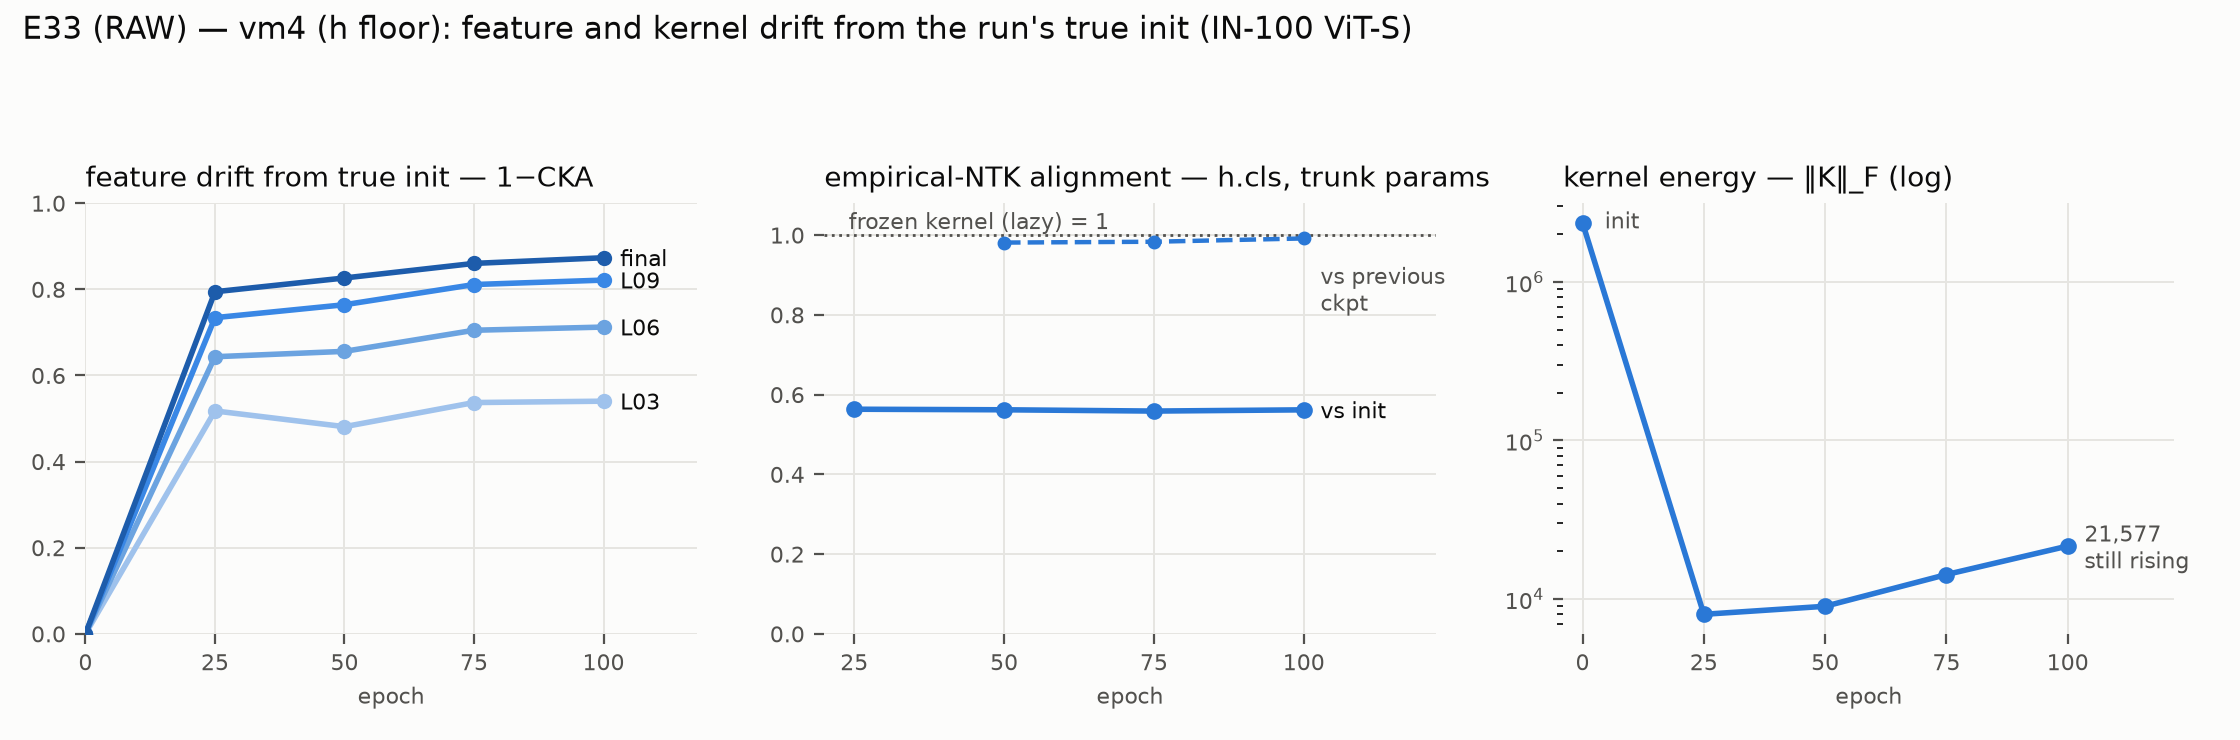
\includegraphics[width=\textwidth]{figures/e33_feature_drift.png}
    \caption{
    Training remains in the rich feature-learning regime. Backbone features move substantially from initialization, and the empirical tangent kernel differs strongly from its initial value.
    }
    \label{fig:rich-learning}
\end{figure*} 






\section{Implementation of the regularizer}
\label{app:slicing}

\paragraph{Invariance objective.}
For image $i$ with $V$ augmented views, we use the mean squared distance between all pairs of projected representations,
\[
\mathcal L_{\mathrm{SSL}}
=
\frac{1}{N}\sum_{i=1}^{N}
\frac{2}{V(V-1)}
\sum_{j<k}
\frac{1}{d_z}
\left\|z_i^{(j)}-z_i^{(k)}\right\|_2^2 ,
\]
where $N$ is the number of images in the batch and $d_z$ is the projector dimension.
This objective contains neither negatives nor an anti-collapse term.
Using $\bar z_i=\frac{1}{V}\sum_{j=1}^{V}z_i^{(j)}$, it is equivalently
$\frac{2V}{V-1}$ times the average squared distance from each view to its image center.
All runs use global views of a single size: $V=4$ on ImageNet-100 and $V=6$ on ImageNet-1k and video.
The invariance and regularization weights are set jointly as described in Appendix~\ref{app:exp-details}.

\paragraph{Slicing.}
For $N$ view centers in $\mathbb R^d$, the centered empirical covariance has rank at most $N-1$.
Thus, when $d\geq N$, the full log-determinant is degenerate.
At each step, we draw a random orthonormal projection
$U\in\mathbb R^{d\times d'}$ using a thin QR factorization of a Gaussian matrix and evaluate
$\mathcal R_{\mathrm{ctr}}$ on the projected centers $XU$.
The same projection is shared across GPUs and resampled every step.
Within the slice, we compute the mean $\mu$ and covariance $\Sigma$ and use $\varepsilon=10^{-4}$.
We divide the regularizer by $d'$, making its scale approximately independent of the slice width.

We use $d'=128$ after the projector ($d_z=256$).
At the backbone, we use one third of the feature width:
$d'=128$ for ViT-S ($d=384$) and $d'=256$ for ViT-B ($d=768$).
The backbone and projector regularizers use independent random slices.

\subsection{Relation to the full-covariance regularizer}
\label{app:slicing-theory}

For clarity, consider the idealized case $\varepsilon=0$.
Let $\mu\in\mathbb R^d$ and $\Sigma\succ0$ denote the mean and covariance
of the view centers. The full regularizer per dimension is
\[
\mathcal R(\mu,\Sigma)
=
\frac{1}{2d}
\left(
\|\mu\|_2^2+\operatorname{tr}\Sigma-d-\log\det\Sigma
\right).
\]

For an orthonormal frame $U\in\mathbb R^{d\times d'}$, the projected
centers have mean $U^\top\mu$ and covariance $U^\top\Sigma U$, giving
the sliced regularizer
\[
\mathcal R_U(\mu,\Sigma)
=
\frac{1}{2d'}
\left(
\|U^\top\mu\|_2^2
+\operatorname{tr}(U^\top\Sigma U)
-d'
-\log\det(U^\top\Sigma U)
\right).
\]
Since a fresh Haar-random frame is sampled at every step, the
corresponding expected slice objective is
\[
\bar{\mathcal R}_{d'}(\mu,\Sigma)
=
\mathbb E_U[\mathcal R_U(\mu,\Sigma)].
\]

\begin{proposition}[Random slicing]
For every $1\le d'\le d$:

\begin{enumerate}[leftmargin=*]
\item[(i)] $\bar{\mathcal R}_{d'}\ge0$, with equality if and only if
$\mu=0$ and $\Sigma=I_d$.

\item[(ii)] The normalized mean and total variance are preserved in
expectation:
\[
\mathbb E_U\frac{\|U^\top\mu\|_2^2}{d'}
=
\frac{\|\mu\|_2^2}{d},
\qquad
\mathbb E_U\frac{\operatorname{tr}(U^\top\Sigma U)}{d'}
=
\frac{\operatorname{tr}\Sigma}{d}.
\]

\item[(iii)] The expected sliced objective approaches the full one
monotonically:
\[
\bar{\mathcal R}_{d'}
\le
\bar{\mathcal R}_{d'+1}
\le
\mathcal R,
\qquad
\bar{\mathcal R}_{d}=\mathcal R.
\]
\end{enumerate}
\end{proposition}

Thus, slicing does not change the preferred representation: averaging
over random subspaces still uniquely favors zero mean and isotropic
unit covariance. The mean and total variance are preserved exactly in
expectation, while the log-determinant observes only the spectrum inside
the sampled subspace. Wider slices therefore capture progressively more
of the full spectral penalty, recovering the original regularizer when
$d'=d$. In practice, we choose $d'<d$ so that the projected covariance
can be estimated from substantially more centers than dimensions.

\paragraph{Proof.}
Each $\mathcal R_U$ is nonnegative and is minimized when
$U^\top\mu=0$ and $U^\top\Sigma U=I_{d'}$. If this holds for all random
subspaces, then every one-dimensional direction has zero projected mean
and unit variance, implying $\mu=0$ and $\Sigma=I_d$.

Haar invariance gives
\[
\mathbb E_U[UU^\top]=\frac{d'}{d}I_d,
\]
which directly yields (ii). Finally, concavity of the logarithm gives
\[
\frac{1}{d'}\mathbb E_U
\log\det(U^\top\Sigma U)
\ge
\frac{1}{d}\log\det\Sigma.
\]
Together with (ii), this gives
$\bar{\mathcal R}_{d'}\le\mathcal R$.
Applying the same argument to a random $d'$-dimensional subspace inside
a random $(d'+1)$-dimensional subspace gives
$\bar{\mathcal R}_{d'}\le\bar{\mathcal R}_{d'+1}$.
For $d'=d$, $U$ is orthogonal and the two objectives are identical.


\paragraph{Ring buffer.}
Reliable covariance estimation requires more centers than the slice dimension.
For each regularized space, we therefore maintain a FIFO buffer containing detached view centers from the previous $q$ steps and concatenate them with the current batch before computing the regularizer.
This gives
\[
N_{\mathrm{eff}}=(q+1)N,
\]
where only the current $N$ centers carry gradients.
Under data parallelism, the buffer contains centers from the full global batch.

We keep $N_{\mathrm{eff}}/d'=4$ throughout image training.
Thus, $q=3$ after the projector and at the ViT-S backbone
($N_{\mathrm{eff}}=512$, $d'=128$), while $q=7$ at the ViT-B backbone
($N_{\mathrm{eff}}=1024$, $d'=256$).
On video, the larger batch sizes reduce the need for buffering:
no buffer is used for ViT-S, while ViT-B uses $q=1$ at the backbone.
We observed no measurable effect from the short parameter lag introduced by the buffered centers.

\paragraph{Averaged invariance target.}
For ImageNet-1k and video, we follow LeJEPA and compute the invariance target using an exponential moving average of the backbone and projector. The target $\tilde z_i$ is the mean projected representation of the $V$ views under the averaged network, and we use
\[
\mathcal L_{\mathrm{SSL}}
=
\frac{2V}{V-1}\,
\frac{1}{N V d_z}
\sum_{i=1}^{N}\sum_{j=1}^{V}
\left\|z_i^{(j)}-\tilde z_i\right\|_2^2 .
\]

ImageNet-100 uses the pairwise objective directly. In all cases, $\mathcal R_{\mathrm{ctr}}$ is computed from view centers of the current network.



\section{Experimental Details}
\label{app:exp-details}

\subsection{Datasets}
ImageNet-1k is the standard split with 1.28M training and 50k validation images. ImageNet-100 is the 100-class subset introduced by CMC (CITE), with 126{,}689 training and 5{,}000 validation images. For video we follow LeVJEPA: we take the union of the Kinetics-400, -600 and -700 training sets, remove duplicates and every clip that appears in a validation set, and keep 20\% of the clips of each class (120{,}100 clips after decoding). LeVJEPA does not release its subset, so ours is a different draw of the same size. Transfer uses DTD, Aircraft, Cars, CIFAR10, CIFAR100, Flowers, Food and Pets (CITE) with the splits of the VISReg protocol; video encoders are evaluated on ImageNet-1k, Something-Something-v2 and Kinetics-400 (CITE).

\subsection{Models and training}
\paragraph{Large-scale image runs.}
We train ViT-S/16 and ViT-B/16 at $224^2$ with a two-layer projector (hidden width 2048, output 256, BatchNorm), batch size 128 split over two GPUs, for 100 and 400 epochs. Each image gives $V=6$ global views from the LeJEPA augmentation family: random resized crops covering 30--100\% of the image, horizontal flips, color jitter, random grayscale, Gaussian blur, and solarization on one of the views. We do not use local crops. Appendix~\ref{app:slicing} describes the slices and buffers are as described there. Optimization uses AdamW with learning rate $10^{-3}$, weight decay $0.05$, 10 warm-up epochs followed by a cosine schedule, gradient clipping at 1.0, and bf16 precision. The loss weights are $(31.07,\,225.50,\,1.671)$ for ViT-S and $(22.81,\,222.26,\,4.054)$ for ViT-B, for the invariance term, $\beta_z$ and $\beta_h$ respectively; they are set as described below and shared by the 100- and 400-epoch runs.

\paragraph{Controlled experiments on ImageNet-100.}
All controlled runs use ViT-S/16 at $224^2$, 100 epochs, batch size 128 and a single seed. We re-implemented LeJEPA, VICReg, SimCLR, DINO, BYOL and VISReg in one training codebase, keeping each method's released loss, projector and augmentation settings. Each method is trained once as released, and once with $\beta_h\mathcal R_{\mathrm{ctr}}(\bar H)$ added and everything else unchanged, so the two runs differ only in the added term. The term is attached to the representation each method passes to its projector: the CLS token for SimCLR, BYOL, VICReg and DINO and the 512-dimensional embedding layer that precedes the projector for LeJEPA and VISReg. Our own objective uses $V=4$ views and the pairwise invariance term of Appendix~\ref{app:slicing}, with weights $32.8$ (invariance), $157.8$ ($\beta_z$) and $1.894$ ($\beta_h$); the unregularized twin sets $\beta_h=0$.

\paragraph{Video.}
We use LeVJEPA's training pipeline and released configuration unchanged except for the loss: their video ViT-S/16 and ViT-B/16 (16 frames at stride 2, tubelet size 1, 95\% token drop), their projector, and their optimizer (AdamW, learning rate $4\times10^{-4}$, weight decay $0.04$, warm-up over 12\% of training followed by a constant learning rate, bf16). Our loss takes $V=6$ global $224^2$ views of the same clip. The batch size is 768 for ViT-S and 512 for ViT-B, the loss weights are those of the image run of the same model size, and we evaluate the exponential-moving-average encoder, as LeVJEPA does.

\subsection{Setting the loss weights}
\label{app:loss-weights}
The loss terms have different forms and scales, so we do not balance them by their values but by their realized pull on the backbone. For a term with weight $w$, let $g$ be the norm of the gradient of the unweighted term with respect to the backbone parameters, measured on a fixed batch at a given checkpoint. The product $w\,g$ is the pull of the term, and its share of the total pull is $w\,g/\sum_k w_k g_k$.

\paragraph{Adding the backbone term to an existing method.}
When adding $\beta_h\mathcal R_{\mathrm{ctr}}(\bar H)$ to an existing SSL method, we choose $\beta_h$ so that the backbone regularizer contributes a small fraction $T=0.06$ of the sum of weighted backbone-gradient norms. Let
\[
G_{\mathrm{SSL}}=\sum_k w_k g_k
\]
denote the contribution of the method's original loss terms, measured at its epoch-25 checkpoint. We set
\[
\beta_h=\frac{T}{1-T}\frac{G_{\mathrm{SSL}}}{g_R},
\]
using a fixed reference $g_R=0.30$ for the gradient norm of $\mathcal R_{\mathrm{ctr}}$. We use a fixed reference because this gradient can be unusually large at a collapsed backbone, which would otherwise yield an artificially small weight. The target share $T=0.06$ was chosen from an earlier dose study on LeJEPA. Thus, $T$ and $g_R$ are fixed across methods, and $\beta_h$ is determined from the scale of each method's existing objective rather than tuned separately.

This gives $\beta_h=0.098$ (SimCLR), $0.0205$ (BYOL), $1.548$ (VICReg), $0.258$ (DINO), $0.0146$ (LeJEPA), and $0.0123$ (VISReg; measured from a one-epoch pilot). For DINO, this weight reduced both linear and kNN accuracy, so we tested $\{0.115,0.02,0.01\}$ and use $\beta_h=0.01$, selected by the online probe.

\paragraph{Our standalone objective.}
For our standalone objective, we set the three loss weights jointly. After a one-epoch pilot, we measure the backbone gradient norm $g_k$ of each term and choose
\[
w_k = 57\,\frac{s_k}{g_k},
\]
with target shares $(s_{\mathrm{inv}},s_{\mathrm{proj}},s_{\mathrm{back}})=(0.44,0.54,0.02)$. These shares and the total magnitude $57$ come from an earlier ViT-S run, and we use the same calibration rule for ViT-S and ViT-B without further tuning.

\subsection{Evaluation}
\paragraph{ImageNet-1k linear probe and kNN.}
We follow the linear-evaluation recipe of the Lightly benchmark (the MAE linear-probe recipe): a BatchNorm layer without affine parameters followed by a linear classifier on the frozen CLS token, trained for 90 epochs with random resized crops and flips, SGD with momentum 0.9 (equivalent to LARS at zero weight decay), learning rate $0.1\times\mathrm{batch}/256$ with a cosine schedule and 10 warm-up epochs; we report the best validation top-1 over the 90 epochs. The kNN classifier uses $k=200$ neighbours with cosine similarity weighted at temperature $0.07$, on the CLS features of the training set.

\paragraph{Transfer.}
We use the VISReg transfer protocol: the CLS tokens of the last four blocks are concatenated, a linear classifier is trained for 10 epochs over a grid of 13 learning rates, and the best test accuracy is reported for each dataset; the table reports the average over the eight datasets. Our implementation reproduces the published DINO ViT-B/16 row within 0.4 points on every dataset.

\paragraph{ImageNet-100.}
The linear probe is a linear classifier on the raw CLS features, trained with AdamW (learning rate $10^{-3}$, weight decay $10^{-7}$) until validation accuracy stops improving; the kNN classifier uses $k=200$ and temperature $0.1$. Both are fit on a fixed subset of 500 training images per class and evaluated on the 5{,}000 validation images.

\paragraph{Video.}
We follow the frozen-encoder protocols of V-JEPA as used by LeVJEPA. ImageNet-1k and Something-Something-v2 use an attentive probe: one cross-attention block with a learnable query over all output tokens followed by a linear classifier, trained for 20 epochs with AdamW (learning rate $10^{-3}$, cosine schedule). For ImageNet-1k each image is repeated over the 16 input frames; for Something-Something-v2 a video is sampled as 2 clips of 16 frames with 3 spatial crops. Kinetics-400 uses a linear classifier on the mean of all output tokens, over 8 clips of 16 frames per video. LeVJEPA does not release the settings of this linear classifier; a classifier trained for 20 epochs with the attentive-probe settings stops well short of the optimum of this convex problem (35.5\% against 43.4\% for our ViT-B at 1{,}085 epochs), so we solve it to convergence with L-BFGS (multinomial logistic regression on standardized features, the best of three ridge strengths $\{10^{-5},10^{-4},10^{-3}\}$) using one center crop per clip and the full training and validation sets. Table~\ref{tab:video-main} reports this number, together with the same classifier on the CLS token and the attentive probe.

\paragraph{Representation statistics.}
All statistics are computed on frozen features. RankMe~\citep{rankme2023} is the exponential of the entropy of the normalized singular values; effective rank is the participation ratio $(\sum_k\lambda_k)^2/\sum_k\lambda_k^2$ of the covariance eigenvalues $\lambda_k$; both are reported as a fraction of the feature dimension. The spectral-tail exponent is the negative slope of $\log\lambda_k$ against $\log k$ over the 200 largest eigenvalues (0 for a flat spectrum, larger for a steeper decay). The stable-center rank is the number of eigenvalues of the between-image covariance $B_h$ (Section~\ref{sec:exp-thickness}, estimated as described next) that exceed $10^{-3}$ of its largest eigenvalue. Positive- and negative-pair cosines are the mean cosine similarity between two views of the same image and between views of two different images.

\paragraph{Augmentation thickness.}
For every model we store $V=8$ augmented views of 10{,}000 training images (100 per class), drawn from the model's own training augmentations, and estimate the two covariances of Section~\ref{sec:exp-thickness} from them: $A_h$ as the average within-image covariance of the views, and $B_h$ as the covariance of the view means minus $A_h/V$, which removes the bias of estimating a center from $V$ views. The scalar thickness reported per model is $\operatorname{tr}A_h/\operatorname{tr}B_h$, i.e.\ the mean squared distance between two views of one image divided by the mean squared distance between two image centers. For the per-class analysis of Figure~\ref{fig:organization-sensitivity}, we whiten the image centers with $B_h$, regress each class indicator linearly on the whitened centers of the training subset, and take the coefficient vector as the class direction $a_c$: the residual of this regression is the organization term $d_h^2$, and $a_c^\top\Theta_h(I+\Theta_h)^{-1}a_c$ is the view-sensitivity term of Eq.~\eqref{eq:too-thick}.

\subsection{Baselines}
OK-AI (CITE) releases LeJEPA, DINO and iBOT trained under one modernized code base at ViT-S and ViT-B for 100 and 300 epochs; we evaluate these checkpoints under the protocols above. Their model card lists 1.45M training images, which is more than the standard ImageNet-1k training split; we did not correct for this. We also trained VISReg ViT-B/16 for 100 epochs with the authors' code and their released view configuration (four global and six local crops), and evaluated the public MoCo~v3, DINO, iBOT and VISReg checkpoints (300--400 epochs) the same way. Transfer numbers marked $^\ddag$ are taken from the VISReg paper. Video baselines are taken from the LeVJEPA paper: the 240-epoch numbers from its Figure~2 and the remaining rows from its equal-compute table.


\subsection{Detailed results}
\label{app:detailed-results}
\begin{table}[h]
\centering
\caption{Per-dataset linear-probe transfer accuracy (\%) under the VISReg protocol; the last column is the average reported in Table~\ref{tab:transfer-main}. $^\ddag$Numbers reported by the VISReg paper; all other rows are evaluated by us under the matched protocol.}
\label{tab:transfer-full}
\resizebox{\textwidth}{!}{%
\begin{tabular}{llrrrrrrrrrr}
\toprule
Method & Backbone & Ep. & DTD & Aircraft & Cars & CIFAR10 & CIFAR100 & Flowers & Food & Pets & Avg. \\
\midrule
LeJEPA (OK-AI) & ViT-S/16 & 100 & 69.4 & 43.8 & 43.4 & 89.3 & 71.1 & 84.0 & 73.6 & 75.3 & 68.7 \\
DINO (OK-AI) & ViT-S/16 & 100 & 69.3 & 55.2 & 57.0 & 93.8 & 78.6 & 89.3 & 76.7 & 85.9 & 75.7 \\
iBOT (OK-AI) & ViT-S/16 & 100 & 69.3 & 55.3 & 56.1 & 93.3 & 77.4 & 90.3 & 77.9 & 87.3 & 75.9 \\
\textbf{Ours} & \textbf{ViT-S/16} & \textbf{100} & \textbf{71.1} & \textbf{55.5} & \textbf{62.5} & \textbf{95.3} & \textbf{81.6} & \textbf{90.4} & \textbf{75.3} & \textbf{89.1} & \textbf{77.6} \\
\midrule
LeJEPA (OK-AI) & ViT-S/16 & 300 & 70.2 & 47.6 & 50.3 & 92.1 & 74.4 & 85.8 & 75.7 & 79.1 & 71.9 \\
DINO (OK-AI) & ViT-S/16 & 300 & 71.5 & 59.8 & 66.2 & 95.0 & 81.1 & 92.0 & 79.6 & 89.6 & 79.4 \\
iBOT (OK-AI) & ViT-S/16 & 300 & 71.6 & 59.7 & 63.3 & 96.0 & 82.4 & 91.2 & 80.9 & 90.6 & 79.5 \\
\textbf{Ours} & \textbf{ViT-S/16} & \textbf{400} & \textbf{71.8} & \textbf{57.9} & \textbf{67.9} & \textbf{95.5} & \textbf{81.8} & \textbf{90.3} & \textbf{78.1} & \textbf{90.7} & \textbf{79.3} \\
\midrule
LeJEPA (OK-AI) & ViT-B/16 & 100 & 72.3 & 51.5 & 54.4 & 93.0 & 76.4 & 86.9 & 78.9 & 80.1 & 74.2 \\
DINO (OK-AI) & ViT-B/16 & 100 & 70.0 & 58.1 & 61.9 & 95.8 & 82.0 & 89.9 & 79.7 & 88.7 & 78.3 \\
iBOT (OK-AI) & ViT-B/16 & 100 & 71.9 & 61.1 & 66.8 & 97.0 & 84.2 & 91.5 & 82.8 & 90.1 & 80.7 \\
VISReg & ViT-B/16 & 100 & 73.3 & 53.1 & 58.0 & 94.3 & 79.6 & 87.9 & 79.1 & 85.5 & 76.4 \\
\textbf{Ours} & \textbf{ViT-B/16} & \textbf{100} & \textbf{71.5} & \textbf{59.8} & \textbf{71.1} & \textbf{96.7} & \textbf{84.9} & \textbf{92.2} & \textbf{79.4} & \textbf{91.7} & \textbf{80.9} \\
\midrule
LeJEPA (OK-AI) & ViT-B/16 & 300 & 73.7 & 52.0 & 55.0 & 93.5 & 77.6 & 87.7 & 80.5 & 81.8 & 75.2 \\
DINO (OK-AI) & ViT-B/16 & 300 & 71.8 & 59.1 & 63.8 & 96.0 & 83.4 & 90.0 & 80.5 & 89.9 & 79.3 \\
iBOT (OK-AI) & ViT-B/16 & 300 & 74.5 & 62.0 & 68.8 & 97.4 & 86.2 & 93.0 & 84.2 & 92.2 & 82.3 \\
MoCo v3$^\ddag$ & ViT-B/16 & 300 & 73.7 & 57.9 & 67.5 & 96.9 & 85.2 & 91.5 & 81.8 & 89.8 & 80.5 \\
DINO$^\ddag$ & ViT-B/16 & 400 & 74.3 & 63.6 & 73.9 & 96.5 & 85.0 & 94.6 & 83.1 & 93.6 & 83.1 \\
iBOT$^\ddag$ & ViT-B/16 & 400 & 74.1 & 63.5 & 73.8 & 97.1 & 85.9 & 93.7 & 84.2 & 93.6 & 83.2 \\
VISReg$^\ddag$ & ViT-B/16 & 400 & 75.7 & 57.1 & 64.8 & 94.6 & 78.8 & 90.4 & 82.9 & 88.3 & 79.1 \\
\textbf{Ours} & \textbf{ViT-B/16} & \textbf{400} & \textbf{73.2} & \textbf{61.1} & \textbf{74.0} & \textbf{96.9} & \textbf{85.4} & \textbf{92.0} & \textbf{81.0} & \textbf{92.2} & \textbf{82.0} \\
\bottomrule
\end{tabular}%
}
\end{table}


\section{A closer look at LeJEPA}
\label{app:lejepa}

Our results suggest that anti-collapse should act on the representation retained for downstream tasks. A natural alternative explanation is that the particular regularizer is unimportant: perhaps simply applying an existing anti-collapse objective at the backbone is sufficient. We test this with LeJEPA, one of the explicitly regularized methods in our study.

LeJEPA encourages the projected representation to match an isotropic Gaussian using SIGReg, a sketched Gaussianity test over random one-dimensional projections. However, its retained backbone representation is far from this target (Figure~\ref{fig:hz_geometry}). Starting from vanilla LeJEPA, with the original SIGReg and invariance losses after the projector unchanged, we therefore add a second SIGReg term directly to the 512-dimensional encoder output, using the weighting heuristic of Appendix~\ref{app:loss-weights}, and train under the ImageNet-100 setup of Section~\ref{sec:exp-in100}.

Table~\ref{tab:lejepa-sigreg} shows that the added SIGReg substantially improves several Gaussianity statistics at the backbone. Negative-pair cosine drops from $0.58$ to $0.01$, the diagonal Gaussian KL from $0.96$ to $0.07$, and the Epps--Pulley statistic also decreases. However, the covariance spectrum remains concentrated: RankMe$/d$ changes only from $0.07$ to $0.09$, while the full-covariance KL remains high ($3.89\to3.03$). At the same time, positive-pair cosine decreases and downstream performance worsens by $1.4$ linear-probe points and $4.3$ kNN points. Thus, the gains from SACReg are not explained simply by moving LeJEPA's existing anti-collapse constraint to the retained representation. In this comparison, directly controlling the covariance spectrum is important: SIGReg substantially improves its Gaussianity diagnostics but leaves the backbone spectrum concentrated, whereas $\mathcal{R}_{\mathrm{ctr}}$ acts explicitly on that spectrum through its log-determinant term.
\begin{table}[h]
\centering
\small
\begin{tabular}{lrr}
\toprule
Readout at encoder output ($h$) & LeJEPA & + SIGReg at $h$ \\
\midrule
Positive-pair cosine & 0.96 & 0.73 \\
Negative-pair cosine & 0.58 & 0.01 \\
KL to $\mathcal N(0,1)$ (diagonal) & 0.96 & 0.07 \\
KL to $\mathcal N(0,I)$ (full covariance) & 3.89 & 3.03 \\
Epps--Pulley & 652 & 504 \\
RankMe$/d$ & 0.07 & 0.09 \\
Linear probe (\%) & 60.4 & 58.9 \\
kNN, $k=200$ (\%) & 52.4 & 48.1 \\
\bottomrule
\end{tabular}
\caption{Adding SIGReg directly to the LeJEPA encoder output on ImageNet-100. The original projector losses are unchanged. All representation statistics are measured at the 512-dimensional encoder output.}
\label{tab:lejepa-sigreg}
\end{table}


\section{Proof of Theorem~\ref{thm:thickness}}
\label{app:thickness}

Let
\[
m_h(Q)=\mathbb{E}[H\mid Q],
\qquad
\xi_h = H-m_h(Q).
\]
We consider the directions in which the image centers have nonzero variance and whiten them, so that
\[
\operatorname{Cov}(m_h(Q))=I,
\qquad
\mathbb{E}[\xi_h\mid Q]=0,
\qquad
\operatorname{Cov}(\xi_h)=\Theta_h.
\]
Let $\mathcal M_h$ denote the set of linear functions of the image centers. Then
\[
d_h(y)
=
\min_{g\in\mathcal M_h}
\|y-g\|_{L_2}.
\]

\paragraph{Too little thickness.}
Consider any linear function of the image centers,
\[
g(Q)=a^\top m_h(Q).
\]
Since $a^\top H$ can be computed from a single augmented view, it is one possible predictor of $g$. Therefore,
\begin{align}
E_{\mathcal A}(g)
&\leq
\mathbb{E}\!\left[
    \left(a^\top m_h(Q)-a^\top H\right)^2
\right] \\
&=
a^\top \Theta_h a.
\label{eq:app-thin-1}
\end{align}

Now let $g$ be the best linear prediction of $y$ from the image centers. Since the image-center covariance is whitened, we can write
\[
g(Q)=a_y^\top m_h(Q),
\qquad
\|a_y\|=\|g\|_{L_2}\leq \|y\|_{L_2}\leq 1.
\]
Using the triangle inequality,
\begin{align}
\sqrt{E_{\mathcal A}(y)}
&\leq
\|y-g\|_{L_2}
+
\sqrt{E_{\mathcal A}(g)} \\
&\leq
d_h(y)
+
\sqrt{\|\Theta_h\|_{\mathrm{op}}},
\end{align}
where the second inequality follows from
Eq.~\eqref{eq:app-thin-1} and $\|a_y\|\leq1$.
Rearranging gives
\[
d_h(y)
\geq
\left(
\sqrt{E_{\mathcal A}(y)}
-
\sqrt{\|\Theta_h\|_{\mathrm{op}}}
\right)_+,
\]
which proves the first part of Theorem~\ref{thm:thickness}.

\paragraph{Too much thickness.}
Let
\[
g(Q)=a^\top m_h(Q)
\]
be the best linear prediction of $y$ from the image centers, and write
\[
y=g+r,
\]
where $r$ is the remaining prediction error. By definition,
\[
\mathbb{E}[r\,m_h(Q)]=0,
\qquad
\mathbb{E}[r^2]=d_h(y)^2.
\]
Also, since $\mathbb{E}[\xi_h\mid Q]=0$,
\[
\mathbb{E}[r\,\xi_h]=0.
\]
Thus $r$ is uncorrelated with $H$ and contributes the term $d_h(y)^2$ to the best linear prediction error from $H$.

For the part $g=a^\top m_h(Q)$, we have
\[
\operatorname{Cov}(H)=I+\Theta_h,
\qquad
\operatorname{Cov}(H,m_h(Q))=I.
\]
The best linear prediction error of $g$ from $H$ is therefore
\begin{align}
\mathbb{E}[g^2]
-
\operatorname{Cov}(g,H)
\operatorname{Cov}(H)^{-1}
\operatorname{Cov}(H,g)
&=
a^\top
\left[I-(I+\Theta_h)^{-1}\right]
a \\
&=
a^\top
\Theta_h(I+\Theta_h)^{-1}
a.
\end{align}
Adding the error $r$ gives
\[
\inf_u
\mathbb{E}\!\left[(y-u^\top H)^2\right]
=
d_h(y)^2
+
a^\top
\Theta_h(I+\Theta_h)^{-1}
a.
\]

Finally,
\[
\Theta_h(I+\Theta_h)^{-1}
=
I-(I+\Theta_h)^{-1}.
\]
Therefore, increasing $\Theta_h$ while keeping the image-center organization and the direction $a$ fixed can only increase the second term. This proves the second part of Theorem~\ref{thm:thickness}.


\end{document}
